%% to be called from the project root: file paths are relative to that

\documentclass[a4paper,12pt]{book}

\usepackage[svgnames]{xcolor}
\usepackage{lipsum}  %% dev
\usepackage{dpfloat}
\usepackage{amsmath}
\usepackage{amssymb}
\usepackage{amsthm}
\usepackage{mathrsfs}
\usepackage{xparse}  %% required by physics
\usepackage{physics}
\usepackage{breqn}
\usepackage{bbm}
\usepackage[utf8]{inputenc}
\usepackage{mathtools}
\usepackage[super]{nth}
\usepackage[inline]{enumitem}
\usepackage{graphicx}
\usepackage{subcaption} % https://tex.stackexchange.com/a/43996 + https://tex.stackexchange.com/a/165730
  \captionsetup{subrefformat=parens}
\usepackage{color}

\usepackage[a4paper,lmargin=4cm]{geometry}

\usepackage{multirow}
\usepackage{fancyhdr}
\pagestyle{fancy}  %% prevent long section titles from overflowing page headers
  \fancyhf{}
  \fancyhead[LE]{\thepage}
  \fancyhead[RE]{\textit{\nouppercase{\leftmark}}}
  \fancyhead[LO]{\textit{\nouppercase{\rightmark}}}
  \fancyhead[RO]{\thepage}
\fancypagestyle{nomark}{%
  \fancyhf{}
  \fancyhead[LE]{\thepage}
  \fancyhead[RE]{}
  \fancyhead[LO]{}
  \fancyhead[RO]{\thepage}
}
\setlength{\headheight}{14.5pt}  %% prevent fancyhead Warning.

% https://tex.stackexchange.com/a/1557
% https://tex.stackexchange.com/a/176939
\usepackage[safeinputenc,style=authoryear-icomp,mincitenames=1,maxcitenames=2,uniquelist=minyear,maxbibnames=7,backend=biber]{biblatex}
%\usepackage[safeinputenc,uniquelist=minyear,maxbibnames=7,backend=biber]{biblatex}
\usepackage{environ}
\usepackage{csquotes}
\usepackage{epigraph}
  \setlength{\epigraphwidth}{.66\textwidth}
  \renewcommand{\epigraphsize}{\small}
  \setlength{\epigraphrule}{0.005pt}
  \setlength{\beforeepigraphskip}{.8\baselineskip}
  \setlength{\afterepigraphskip}{1.2\baselineskip}
\usepackage{fancyvrb}
  \fvset{
    frame = single,
    rulecolor=\color{lightgray}
  }
\usepackage{footnote}
%
% Ways to avoid "random" vertical space between paragraphs
% https://tex.stackexchange.com/a/36429
\raggedbottom
\usepackage[bottom]{footmisc}
%
\usepackage{listings}
  \lstset{
    frame = single,
    rulecolor=\color{lightgray},
    basicstyle=\setstretch{1.2}\scriptsize\ttfamily,
    commentstyle=\color{gray},
    keywordstyle=\color{blue},
    stringstyle=\color{red},
    fancyvrb=true,
    breaklines=true,
    aboveskip=1.1em,
    belowskip=0.4em,
    %identifierstyle=\color{green!40!black}
  }
\usepackage{setspace}
\usepackage{etoolbox}
\usepackage[  %% be (almost) the last -- https://tex.stackexchange.com/a/326953
  %% pdfusetitle would not render the ket <1| correctly -- title is a plain text
  pdftitle={It's |1> o'clock -- Relational Time and Applications},
  colorlinks
]{hyperref}
  \hypersetup{
    linkcolor = DarkRed,
    citecolor = Green,
    urlcolor  = DarkBlue
  }

% https://tex.stackexchange.com/a/65547
\usepackage{bookmark}

% "dev only"
\ifdev
  % \usepackage[breakable,skins]{tcolorbox}
  % \definecolor{tcbcolback} {HTML}{EEEEFF}
  % \definecolor{tcbcolframe}{HTML}{4444BB}
  % \tcbset{
  %   colback=tcbcolback, colframe=tcbcolframe,
  %   breakable, enhanced jigsaw,
  %   parbox=false, before upper={%
  %     \setlength{\parskip}{0.666em}%
  %     \setlength{\parindent}{0pt}%
  %     \setstretch{1.2}%
  %   }
  % }

  % https://tex.stackexchange.com/a/53252
  \pdfcompresslevel=0
  \pdfobjcompresslevel=0
\fi

%%%%

%% Theorem-like environments

%% http://www.maths.tcd.ie/~dwilkins/LaTeXPrimer/Theorems.html
%% https://www.sharelatex.com/learn/Theorems_and_proofs
%% http://tex.stackexchange.com/a/46262
\newtheorem{theorem}{Theorem}[section]
\newtheorem{lemma}[theorem]{Lemma}
\newtheorem{proposition}[theorem]{Proposition}
\newtheorem{corollary}{Corollary}[theorem]
\newtheorem{remark}{Remark}[section]
\newcommand{\remarkautorefname}{Remark}

%% Adapted from https://tex.stackexchange.com/q/45817
\theoremstyle{definition}
\newtheorem{definition}{Definition}[section]
\newtheorem{axiom}{Axiom}[section]
\newtheorem{conjecture}{Conjecture}[section]
\newtheorem{example}{Example}[section]

%%%%

\newcommand{\ch}{{c.}\:}             % chapter in bib citations
\newcommand{\s}{{s.}\:}              % section in bib citations
\newcommand{\citeplace}[1]{{#1}\:}   % ``any'' in bib citations  e.g. \cite[\citeplace{handout} 2]{Webber_notes}

\newcommand{\term}[1]{\emph{#1}}
\newcommand{\idop}{\mathbbm{1}}           % Identity operator
\newcommand{\hilb}[1]{\mathcal{#1}}       % Hilbert space
\newcommand{\setof}[1]{\left\{#1\right\}}
\newcommand{\ox}{\otimes}
\newcommand{\transpose}{\top}

%% Allows better formatting than \underset
%% https://tex.stackexchange.com/a/130553
\DeclareMathOperator*{\repr}{\,\equiv\,}      % represented in a basis, or "has components..."

\renewcommand{\op}{\hat}                  % overwriting physics \op = \ketbra
%\renewcommand{\op}{}                      % overwriting physics \op = \ketbra
\newcommand{\eqbydef}{\coloneqq}
%\newcommand{\eqbydef}{\triangleq}
\newcommand{\superop}{\mathcal}

\newcommand{\dket}[1]{\left.\left| #1 \right\rangle\right\rangle}
\newcommand{\Dket}[1]{\left.\left| #1 \right\rangle\!\right\rangle}
\newcommand{\dbra}[1]{\left\langle\left\langle #1 \right|\right.}
\newcommand{\Dbra}[1]{\left\langle\!\left\langle #1 \right|\right.}
\newcommand{\dbraket}[2]{\left\langle\left\langle #1 \middle| #2 \right\rangle\right.\!}
\newcommand{\bradket}[2]{\!\left.\left\langle #1 \middle| #2 \right\rangle\right\rangle}
\newcommand{\braDket}[2]{\!\left.\left\langle #1 \middle| #2 \right\rangle\!\right\rangle}
\newcommand{\dbradket}[2]{\left\langle\left\langle #1 \middle| #2 \right\rangle\right\rangle}
\newcommand{\dketdbra}[2]{\dket{#1}\dbra{#2}}

%% smaller than \quad but still quite larger than \;
\newcommand{\kuad}[0]{\:\:\,}

\newcommand{\pwspace}{\hilb{H}_T \ox \hilb{H}_S}

\NewEnviron{eqsplit}{\begin{equation}\begin{split}\BODY\end{split}\end{equation}}
\NewEnviron{eqsplit*}{\begin{equation*}\begin{split}\BODY\end{split}\end{equation*}}

% Imaginary unit (not used much this way here though)
% https://tex.stackexchange.com/a/303698
\newcommand{\iu}{\mathrm{i}\mkern1mu}
\newcommand{\E}{\mathrm{e}}

% Functions
% Heaviside function
\newcommand{\Hvsd}[1]{\Theta\left(#1\right)}

%\newcommand{\nullvector}{\underline{0}}
\newcommand{\nullvector}{0}


\renewcommand{\arraystretch}{1.6}

% https://tex.stackexchange.com/a/325704
\AtBeginEnvironment{quote}{\singlespace\vspace{-\topsep}}
\AtEndEnvironment{quote}{\vspace{-\topsep}\endsinglespace}

\author{Guido De Rosa \\ \small\tt{gderosa@umail.ucc.ie}}
\title{It's $\ket{1}$ o'clock -- Relational Time and Applications}

\addbibresource{bib/main.bib}
\addbibresource{bib/comp.bib}
\addbibresource{bib/misc.bib}
% For peer-reviewed articles, in general there is a DOI which is detailed enough,
% while only some entries have issn fields, essentially out of a copypaste -
% See also https://tex.stackexchange.com/a/32933.
\AtEveryBibitem{
  \clearfield{issn}
  \clearfield{month}
}


\begin{document}

\frontmatter

\maketitle

\tableofcontents

\listoffigures
 
\listoftables

\chapter*{Preface}
\markboth{Preface}{Preface}  %% No ugly "Chapter 0".
\addcontentsline{toc}{chapter}{Preface}
This work relates to the problem of time in quantum physics%
\footnote{
  See, for a review, \cite{TQM1, TQM2}.
},
from Wolfgang Pauli's argument
on the impossibility of defining a time observable \parencite{PauliFootnote},
to \emph{relational} models developed during the last decades:
according to such models,
time and unitary evolution only emerge in
terms of \emph{entanglement} between noninteracting subsystems
---one of which acts as a ``clock''---
of an otherwise stationary universe \parencite{PageWootters, Marletto:Evolution}.

Pauli's objection is reviewed and commented,
as well as some of the alternate models
that have been proposed
to overcome it.

One of the aims of the present work
is contributing towards bridging a gap between the theoretical
and experimental literature on the topic.
To this end, examples and applications are developed on top of existing theoretical results.
Conversely,
a conceptual critique and theoretical analysis
of recent experiments is carried out.
Numerical computation is also extensively employed in order to compare
predictions from different models, relational or not.

\mainmatter

\if{todo}
\chapter{Motivation and experiments}
\begin{itemize}
  \item Time crystals?
  \item Time-resolved diffraction patters, temporal double slit experiment + Muga theory \url{https://arxiv.org/pdf/0812.3034.pdfß}
\end{itemize}

%\clearpage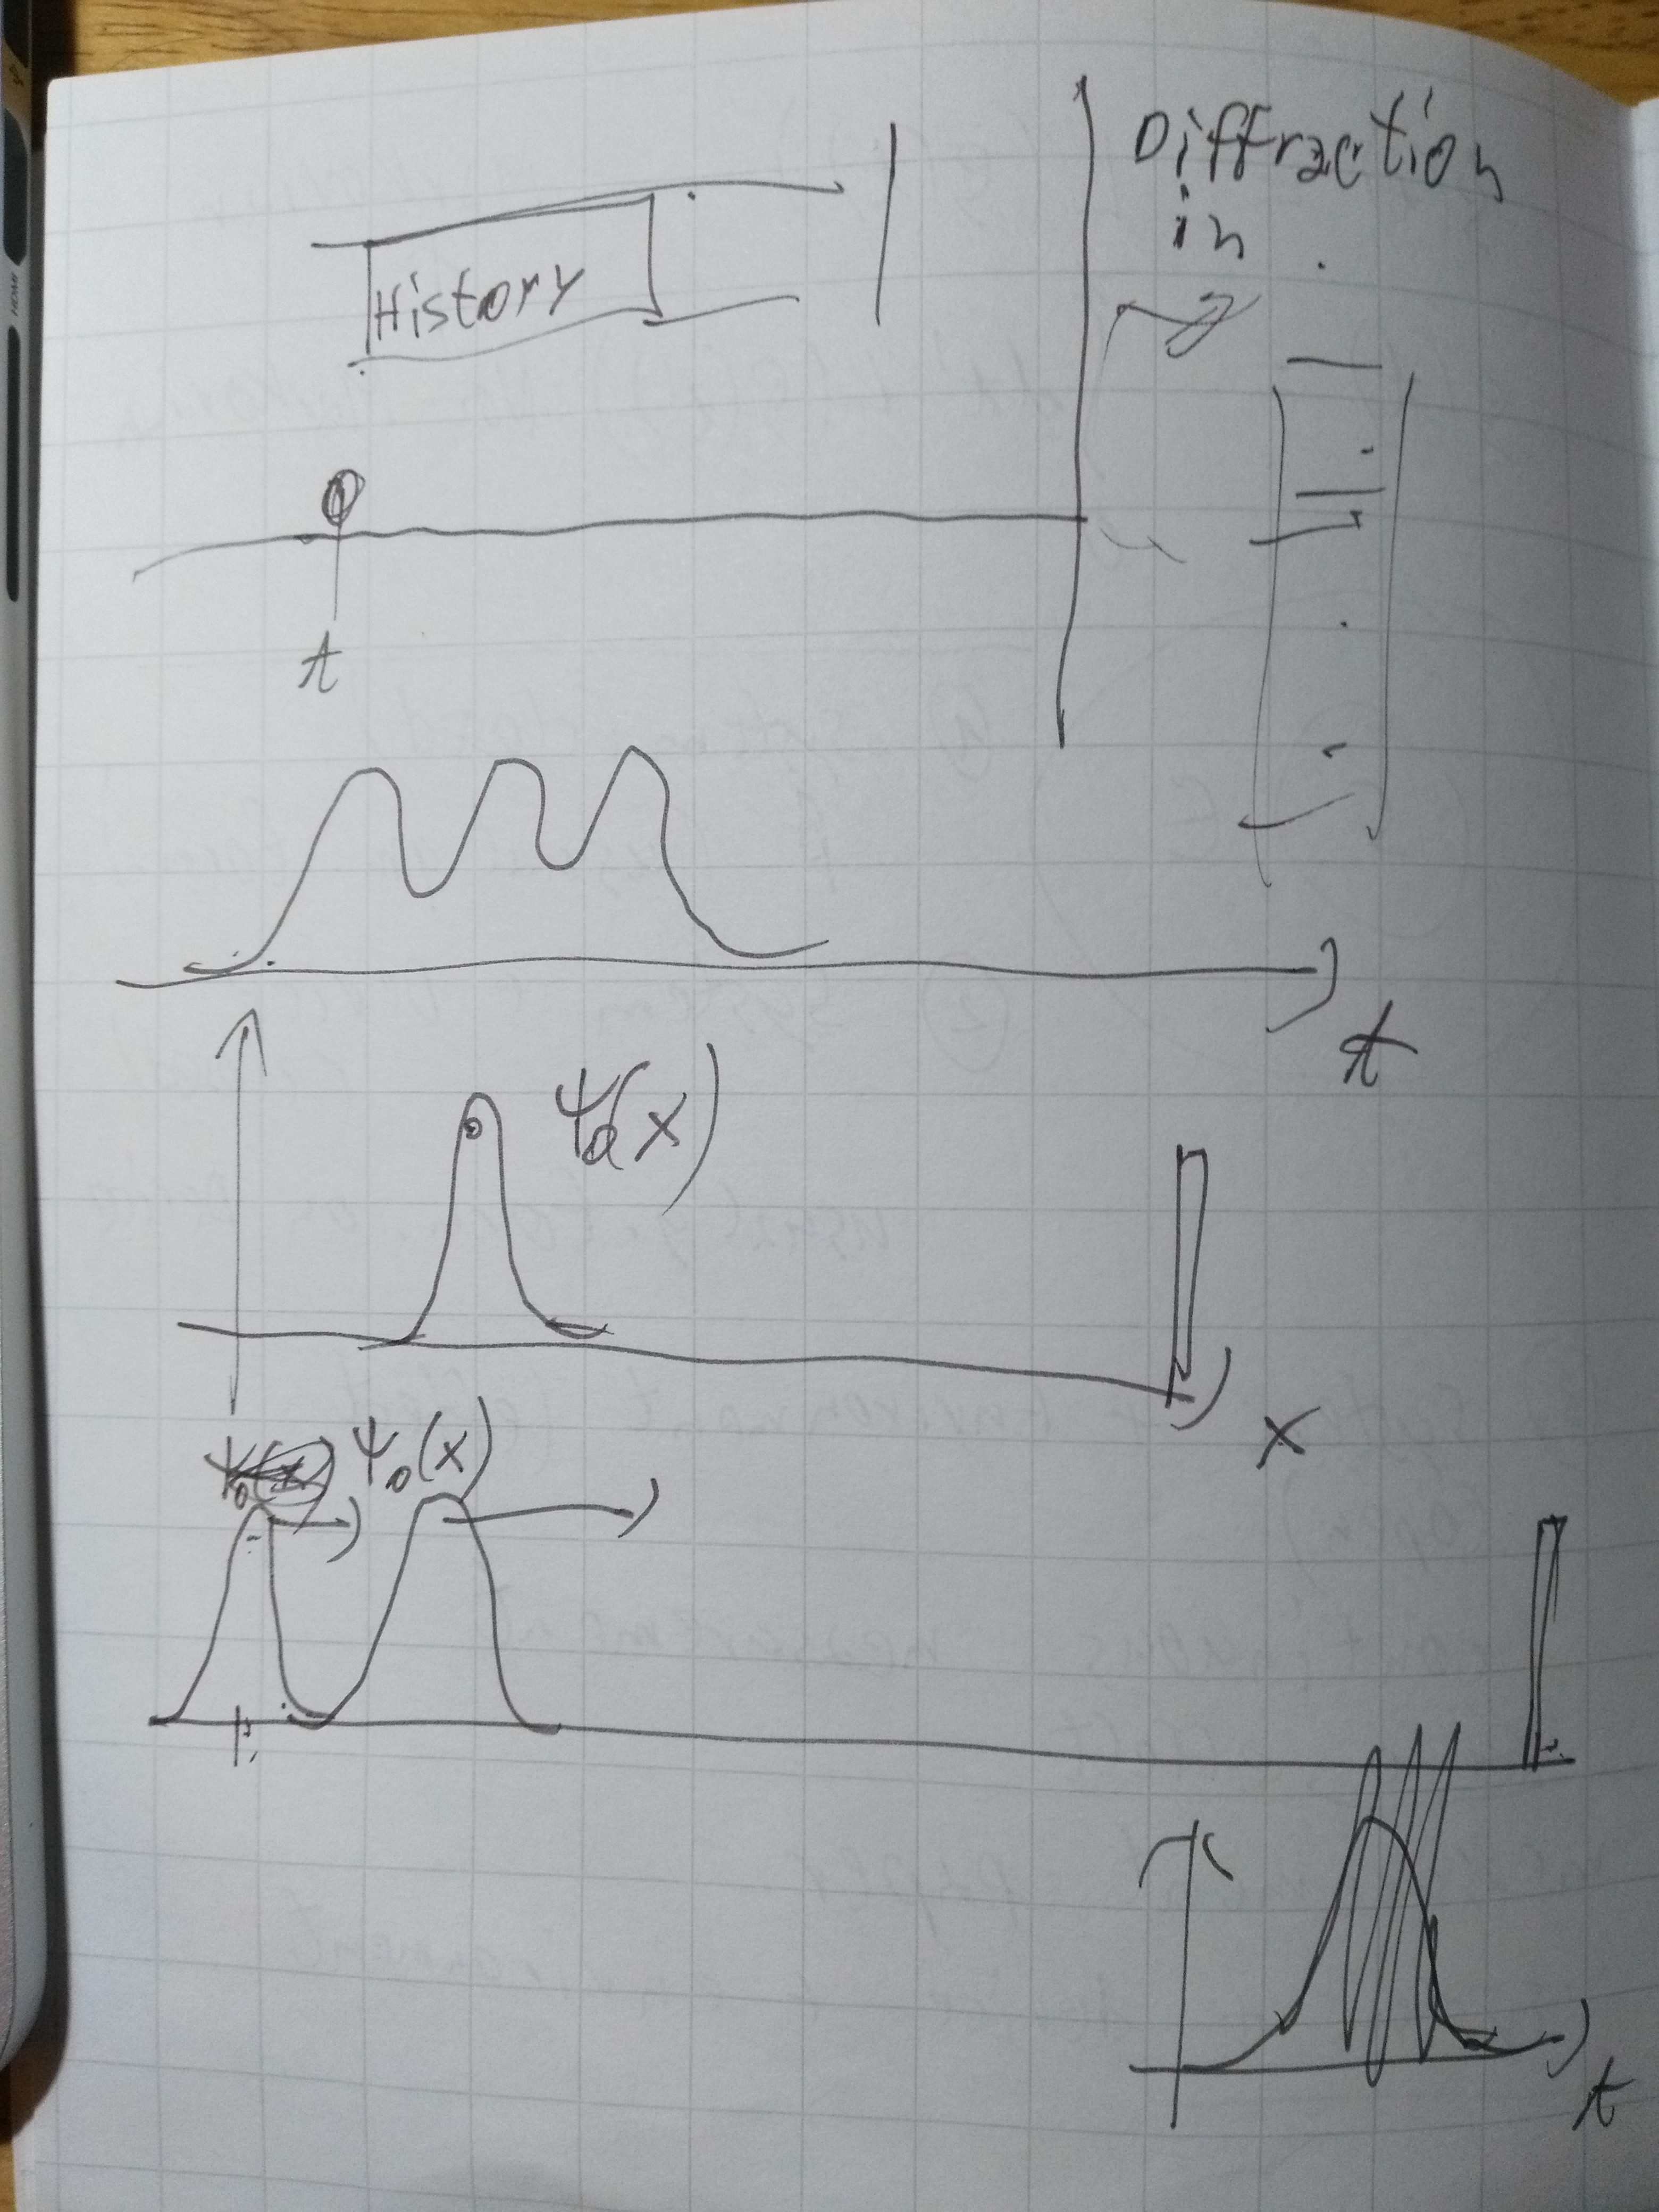
\includegraphics[width=\linewidth]{img/diffraction.jpg}

\fi

\chapter{Pauli's objection and historical developments}
\section{Introduction}

In a footnote in~\cite{PauliFootnote}, W. Pauli excluded the possibility
of a self-adjoint operator representing time as a quantum observable.
However, he did not provide an explicit proof.
Here a proof is given, based on~\cite{Galapon2002}, but expanded in more detail.

\section{Proof of Pauli's formal argument}\label{proof}

Let's assume that there exists a self-adjoint time operator, $T$, canonically conjugate
to the Hamiltonian $H$, i.e.

\begin{equation}
\label{THcommutator}
[T, H] = i\hbar
\end{equation}
Since T is self-adjoint, then for all
$\beta\in\mathbb{R}$, $U_{\beta} = \exp(- i \beta T / \hbar)$
is unitary. A formal
expansion of the exponential yields the commutator

\begin{equation}
[U_{\beta}, H]  =
\left[
    \sum_{k=0}^{\infty} \frac{1}{k!} \left(- \frac{i\beta T}{\hbar} \right)^k, H
\right]         =
\sum_{k=0}^{\infty} \frac{1}{k!} \left(- \frac{i\beta}{\hbar} \right)^k [T^k, H]
\end{equation}.

As the commutator $[T, H]$ itself commutes with its operator $T$,
the following identity holds (See Lemma \ref{CommProp}):

$$
[T^k, H] = kT^{k-1}[T, H]
$$
hence:

\begin{multline}
[U_{\beta}, H]  =
\sum_{k=0}^{\infty} \frac{1}{k!} \left(- \frac{i\beta}{\hbar} \right)^k kT^{k-1}[T, H] \\ =
\beta\sum_{k=1}^{\infty} \frac{1}{(k-1)!} \left(- \frac{i\beta}{\hbar} \right)^{k-1} T^{k-1} =
\beta\sum_{\kappa=0}^{\infty} \frac{1}{\kappa!} \left(- \frac{i\beta T}{\hbar} \right)^{\kappa}  =
\beta U_{\beta}
\end{multline}
where the term for $k=0$ in the first sum clearly vanishes, hence we can start the sum from
$k=1$ then set $\kappa=k-1$.

Now, given an eigenvector $\varphi_{E}$ so that $H\varphi_{E}=E\varphi_{E}$, there has:

$$
HU_{\beta}\varphi_{E} = (U_{\beta}H - [U_{\beta}, H])\varphi_{E} =
EU_{\beta}\varphi_{E} - \beta U_{\beta}\varphi_{E} = (E-\beta)U_{\beta}\varphi_{E}
$$
showing that $U_{\beta}\varphi_{E}$ is another eigenvector of $H$ with eigenvalue
$E-\beta$. But $\beta$ is an arbitrary real number and $H$ a \emph{generic} Hamiltonian,
hence the spectrum of a generic Hamiltonian $H$ should
be the whole real line, which contradicts the discrete and semi-bounded energy spectrum
in fact found in most physical systems.

\section{Von Neumann}
TODO: Andreas' book: expand + Zurek, also recalled in
the section dedicated to quantum-to-classical \ref{sec:q2c}.

\if{todo}
\chapter{Approaches}
\section{Approaches}

They are

\begin{itemize}
\item early attempts reviewed in \cite{TQM1, TQM2}, Aharonov-Bohm, Kijowski etc.
\item detector model \cite{TQM1, TQM2}
\item
    time $\otimes$ position Hilbert space or ``second'' Schr\"odinger equation (Prvanovic)
\item time and entanglement (Page and Wootters model, Leggett-Garg inequality as \emph{time} version of Bell inequalities, experiments by Moreva, Genovese et al.)
\item approachs where not only spacetime but causality itself is not fundamental (indefinite causal order: Oreshkov, Brukner et al)
\item event-based approaches: 
    \begin{itemize}
        \item ``event'' wavefunction square integrable in 4D (how does it relate rigourously to detector model?)
        \item event-enhanced quantum theory (EEQT, Ruschhaupt et al.)
        \item 
    \end{itemize}
\end{itemize}
\fi

\chapter{Decoherence and Measurement}
%% With appendices moved here, this chapter is much less
%% about (reletalively recent) research and more
%% textbook-like.

This chapter is devoted to briefly recall some
foundations and modern developments of quantum measurement theory.
It's strongly based on works like
\cite{PreskillNotes, Haroche_Exploring, Nakahara, NielsenChuang, open_systems},
where they are presented in the context of
open quantum systems and quantum information theory.

\section{Bipartite systems, separable and entangled states}

Consider a \term{bipartite quantum system}
i.e. a composite system $S$
made up of two parts, $A$ and~$B$,
described by their respective Hilbert spaces
$\hilb{H}_A$ and $\hilb{H}_B$.

Notably, in \cite{Haroche_Exploring},
notation does not treat the two spaces
on perfectly equal footing,
in the sense that a basis for $\hilb{H}_A$ and a basis for $\hilb{H}_B$
are indicated as
$$
  \setof{\ket{i_A}} \text{ and } \setof{\ket{\mu_B}}\,
$$
with latin and greek indices to label base vectors in the two spaces.
We will follow such convention unless otherwise specified.

This indicates different physical roles for the two spaces,
such as the \emph{system of interest} and the surrounding \emph{environment},
or the \emph{system being measured} and the \emph{measurement apparatus}.

If the two subsystems are prepared independently and not let interact with each other,
the system is in a \term{product state} or \term{separable state}:
\begin{equation}\label{eq:separableAB}
  \ket{\psi_S} = \ket{\psi_A}\otimes\ket{\psi_A} \,\text{.}
\end{equation}

It's worth recalling that in a tensor product space $\hilb{H}_A\otimes\hilb{H}_B$
not all vectors can be expressed as a tensor product as in \eqref{eq:separableAB}.
However, the following holds:

\begin{proposition}\label{TensorBase}
The set of tensor products of base vectors of $\hilb{H}_A$ and $\hilb{H}_B$,
i.e. $$\setof{\ket{i_A} \otimes \ket{\mu_B}}_{i\mu},$$
is a basis for $\hilb{H}_A \otimes \hilb{H}_B$
\end{proposition}
Therefore, we can express any
(generally not separable) state vector of $\hilb{H}_S$
as a \emph{superposition} of separable base vectors
\begin{equation}\label{eq:bipartite_expansion}
  \ket{\psi_S} = \sum_{i, \mu}\alpha_{i\mu}\ket{i_A}\otimes\ket{\mu_B} \neq \ket{\psi_A}\otimes\ket{\psi_B},
\end{equation}
meaning that the
``total'' $\ket{\psi_A}$ and $\ket{\psi_B}$ don't necessarily exist.

Non separable states are said \term{entangled}.

Physically,
$\ket{\psi_S}$ contains information
not only about the results of measurements on $A$ and $B$ separately,
but also on correlations between these measurements.

The simplest example of entangled system is given by two two-level systems,
namely two spin-$\frac{1}{2}$ particles in a singlet state:
\[
  \ket{\psi_{\text{singlet}}} = \frac{1}{\sqrt{2}} \left(\ket{\uparrow, \downarrow} - \ket{\downarrow, \uparrow}\right).
\]

\section{Density operator}\label{app:density}

A quantum state (either pure or \term{mixed}),
is generally described by a \term{density} operator (or density matrix) $\rho$.

The general expression for a density operator $\rho$ is
$$
  \rho = \sum_{k}p_{k}\ketbra{\psi_{k}}
$$
with $p_{k}$ being non negative and $\sum_{k}p_{k} = 1$;
where $p_k$ indicates the ``classical'' probability of the system to be in state $\ket{\psi_{k}}$.

For a pure state (corresponding to ket $\ket{\psi}$) the density operator reduces to
\[
  \rho_{(\text{pure})} = \ketbra{\psi}\,\text{.}
\]

The expectation value of an observable represented by the operator $A$
is given by \parencite{BlumDensity, FanoDensity}
\begin{equation}\label{eq:expvalA_rho}
  \expval{A} = \tr(A\rho)\,.
\end{equation}

Eq. \eqref{eq:expvalA_rho} is valid for any Hermitian operator $A$. Particularly,
it is also valid if $A$ is a \emph{projector} and we will use this
e.g. in Proposition \ref{probability_rho}.

We will now look at some properties of the density operator.

We can prove the following
\begin{proposition}
  Let $A$ be an Hermitian operator
  a complete set of eigenvectors $\{\ket{m}\}$
  and
  such that
  $$
    \tr(A\rho) = 0
  $$
  \emph{for any density operator} $\rho$.
  It follows that $A = 0$.

  \begin{proof}
    We can choose
    ---to explicitly evaluate the expression of the trace---
    for each positive integer $n$,
    a particular density operator $\rho = \ketbra{n}$,
    corresponding to a (pure) eigenstate of $A$.

    With this particular choice,
    for each $n$,
    $$
      A\rho = \mel{n}{A}{n}\ketbra{n}\,.
    $$
    It then follows:
    \begin{multline}\label{eq:qmt:alldiagzero}
      0 = \tr(A\rho) = \sum_{m}\mel{m}{ ( \mel{n}{A}{n}\ketbra{n} ) }{m} = \\
          \sum_{m} \mel{n}{A}{n} \braket{m}{n} \braket{n}{m}
        = \mel{n}{A}{n} .
    \end{multline}
    With respect to the basis $\setof{\ket{n}}$ the operator $A$ is
    represented by a matrix whose elements are given by $a_{nm} = \mel{n}{A}{m}$;
    but $\setof{\ket{n}}$ is an eigenbasis, therefore we are only interested in the diagonal
    elements (the off-diagonal ones being zero).
    However, the diagonal elements are  $\mel{n}{A}{n} = 0$
    for all $n$, according to Eq.~\eqref{eq:qmt:alldiagzero}, therefore the operator itself is $A=0$.
  \end{proof}
\end{proposition}

The \emph{additivity} property follows immediately:

\begin{corollary}
If $\tr(A\rho) + \tr(B\rho) = \tr(C\rho)$ for any density operator $\rho$,
then $A + B = C$.
\end{corollary}

\section{Partial trace and open systems}
\label{sec:p_tr}

In a bipartite system, one subsystem considered alone is an
\emph{open quantum system},
while the system as a whole is still a closed systems.

Now, let's consider an observable $M_A$, acting only on subsystems $A$.
It can be expressed in $\hilb{H}_A \otimes \hilb{H}_B$ as
\[
  M_A \otimes \idop_B\, .
\]
Its expectation value is
(using the expansion in Eq.~\eqref{eq:bipartite_expansion},
and the notation of Latin indices for system $A$ and Greek ones for system $B$)
\begin{multline}\label{eq:exp_subsys}
  \expval{M_A} = \matrixel{\psi_S}{M_A\otimes\idop_B}{\psi_S} = \\[1em]
  \sum_{j,\nu}a^{*}_{j\nu}\left(\bra{j}\otimes\bra{\nu}\right)\left(M_A\otimes\idop_B\right)\sum_{i,\mu}a_{i\mu}\left(\ket{i}\otimes\ket{\mu}\right) = \\
  \sum_{j,\nu,i,\mu}a^{*}_{j\nu}a_{i\mu}\matrixel{j}{M}{i}\matrixel{\mu}{\idop}{\nu} =
  \sum_{j,\mu,i}a^{*}_{j\mu}a_{i\mu}\matrixel{j}{M}{i}
\end{multline}

The bra $\bra{\mu}$, when acting on a ket element of $\hilb{H}_{A} \ox \hilb{H}_{B}$,
can be defined
as a map from $\hilb{H}_A\otimes\hilb{H}_B$ to $\hilb{H}_A$.

A formal definition can be given in terms of how it acts upon a generic
basis ket of $\hilb{H}_A\otimes\hilb{H}_B$.

\begin{definition}\label{def:pBra}
\[
  \braket{\mu}{i\nu} = \bra{\mu}\Big(\ket{i}\otimes\ket{\nu}\Big) \eqbydef \delta_{\mu\nu}\ket{i} \text{.}
\]
\end{definition}

Intuitively, $\bra{\mu}$ is then a ``partial bra''
as it only maps the ``$\ket{\nu}$'' part of\\
``$\ket{i}\otimes\ket{\nu}$''
to a number:
\[
  \begin{array}{cccc}
    \bra{\mu}:  & \ket{i}\ox\ket{\nu}                   & \rightarrow & \delta_{\mu\nu}\ket{i}                \\
                & \rotatebox[origin=c]{270}{$\in$}      &             & \rotatebox[origin=c]{270}{$\in$}      \\
                & \hilb{H}_A\ox\hilb{H}_B               &             & \hilb{H}_A   \text{.}
  \end{array}
\]

This is consistent with the idea of
``tracing out the environment'' within an interpretation where
$\hilb{H}_B$ is the environment, and ultimately with the goal of
studying subsystem $A$ alone in spite of its entanglement with the
``environment'' (or measurement apparatus etc.) modeled by
subsystem $B$.

Conversely,
the ket $\ket{\mu}$, when acting on a bra element of $\hilb{H}_{A} \ox \hilb{H}_{B}$,
can also be defined
as a map from $\hilb{H}_A\otimes\hilb{H}_B$ to $\hilb{H}_A$.
The following definition of $\ket{\mu}$ is simply \term{dual} to Definition \ref{def:pBra}:
\begin{definition}\label{def:pKet}
  \[
    \braket{i\nu}{\mu} = \Big(\bra{i}\ox\bra{\nu}\Big)\ket{\mu} \eqbydef \delta_{\mu\nu}\bra{i} \text{.}
  \]
\end{definition}
Similar considerations apply:
\[
  \begin{array}{cccc}
    \ket{\mu}:  & \bra{i}\ox\bra{\nu}                   & \rightarrow & \delta_{\mu\nu}\bra{i}               \\
                & \rotatebox[origin=c]{270}{$\in$}      &             & \rotatebox[origin=c]{270}{$\in$}      \\
                & \hilb{H}_A\ox\hilb{H}_B               &             & \hilb{H}_A     \text{.}
  \end{array}
\]

%%

The operations defined (for basis vectors) in Definition \ref{def:pBra} and \ref{def:pKet}
are called \term{partial inner products} \parencite[\s 1.3.3]{QMT_Jacobs}.
They can be extended to all vectors of $\hilb{H}_B$ and $\hilb{H}_B\ox\hilb{H}_B$
simply by linearity.

Similarly, partial inner products with bras and kets of $\hilb{H}_A$
(and values in $\hilb{H}_B$) can be defined as well.

We are now in the position to introduce the \term{partial trace}:
\begin{definition}\label{def:pTr}
  The \term{partial trace}
  is a linear map
  that takes an operator
  $M_{AB}$ on $\hilb{H}_A \otimes \hilb{H}_B$
  to an operator on $\hilb{H}_A$ defined as
  \[
    \tr_B M_{AB} = \sum_{\mu} \matrixel{\mu}{M_{AB}}{\mu}
    \, \text{,}
  \]
  where $\setof{\ket{\mu}}$ is a basis of $\hilb{H}_B$.
\end{definition}

The first thing to note is that the \emph{partial} trace is \emph{operator-valued},
its value is not a scalar as opposed to the \emph{trace}.

Next, we can introduce the \term{reduced density operator}
of system $A$, which is obtained by \emph{tracing out the environment} B,
via the partial trace:
\begin{definition}\label{def:density_A}
  If $\rho$ is the density operator of a whole bipartite system, composed of two parts $A$ and $B$,
  the \term{reduced density operator} related to subsystem $A$ is defined as
  \[
    \rho_A = \tr_B(\rho) \, \text{.}
  \]
\end{definition}

We assume now that the total state $\rho$ is a pure state $\rho = \ketbra{\psi_S}$.

If $\setof{\ket{\mu}}$ is a basis of $\hilb{H}_B$,
for each element $\ket{\mu}$,
using the definitions \ref{def:pBra} and \ref{def:pKet}
and the expansion \eqref{eq:bipartite_expansion}, we obtain
\begin{eqsplit}\label{eq:psiPartial}
  \braket{\mu}{\psi_S} &= \sum_i \alpha_{i\mu}    \ket{i} \text{,} \\
  \braket{\psi_S}{\mu} &= \sum_j \alpha_{j\mu}^{*}\bra{j} \text{.}
\end{eqsplit}

which allows us to expand the definition of reduced density operator (Definition \ref{def:density_A})
as\footnote{
  The key point of this reasoning is showing how
  a pure state of the total system can correspond to mixed states
  in the two subsystems $A$ and $B$. Therefore it is not restrictive to assume,
  in what follows,
  that the total state $\rho = \ketbra{\psi_S}$ is pure.
}

\begin{equation}\label{eq:density_A_expand}
  \rho_A = \tr_B(\ketbra{\psi_S}{\psi_S}) =
    \sum_{\mu}\braket{\mu}{\psi_S}\braket{\psi_S}{\mu} =
    \sum_{ij\mu} \alpha_{i\mu}\alpha_{j\mu}^{*}\ketbra{i}{j} \text{.}
\end{equation}

Finally, we can see that
\begin{multline*}
  \tr(M_A \rho_A) = \sum_k \mel{k}{M_A \rho_A}{k} =
    \sum_k \mel {k} {M_A \left(\sum_{ij\mu} \alpha_{i\mu}\alpha_{j\mu}^{*}\ketbra{i}{j}\right)} {k} = \\
    \sum_{ijk\mu} \alpha_{i\mu}\alpha_{j\mu}^{*} \mel{k}{M_A}{i} \braket{j}{k} =
    \sum_{ij\mu} \alpha_{i\mu}\alpha_{j\mu}^{*} \mel{j}{M_A}{i}
    \, \text{,}
\end{multline*}
which is the same result as \eqref{eq:exp_subsys}.

This allows us to conclude that
\begin{proposition}
  For an observable $M_A$, acting solely on one subsystem, the expectation value
  for state $\rho$ can be calculated as
  \begin{equation}
    \expval{M_A} = \tr(M_A \rho_A)
  \end{equation}
  where $\rho_A$ is the reduced density operator obtained from $\rho$ by
  tracing out the environment $B$ (as per Definition \ref{def:density_A}).
\end{proposition}

It's clear from \eqref{eq:density_A_expand} that $\rho_A$ is self-adjoint,
hence it can be diagonalized:
\begin{equation}\label{eq:rho_diag}
  \rho_A = \sum_a p_a \ketbra{a}{a} \text{.}
\end{equation}

Let $\setof{\ket{k}}$ be a basis of $\hilb{H}_A$.
From \eqref{eq:density_A_expand} we can also derive that
\begin{equation}
  \tr\rho_A = \sum_k \mel{k}{\rho_A}{k} =
    \sum_{ijk\mu}\alpha_{i\mu}\alpha_{j\mu}^{*}\braket{k}{i}\braket{j}{k} =
    \sum_{k\mu}\abs{\alpha_{k\mu}}^2 = 1 \text{,}
\end{equation}
where the last equality is justified by the normalization of $\ket{\psi_S}$
in \eqref{eq:bipartite_expansion}.

The trace, i.e. the sum of matrix diagonal elements, is independent
from the chosen basis, hence $\tr\rho_A = 1$ is valid in particular
for the diagonal form \eqref{eq:rho_diag}, meaning
\[
  \sum_a p_a = 1
\]
and providing a necessary condition to interpret $p_a$ as a probability.

Eq. \eqref{eq:rho_diag}, with $p_a$ as a probability, is often
given as a \emph{definition} of the density operator.
% TODO: do the calculation?
The probability distribution ${p_a}$
is described as a ``classical'' uncertainty in the preparation of the system
(for example due to an unknown interaction with the environment).

The reverse also holds true:
\begin{proposition}
A system with uncertainties in the preparation of the \emph{state}
(``mixed'') is equivalent to one part (``$A$'') of a bipartite system
entangled with the rest (``B'') such that the total system
$A+B$ is in a pure state.
\end{proposition}

The above is called \term{purification} (see e.g. \cite[\s 2.5]{NielsenChuang}).


\section{Comparison of a coherent superposition and a mixed state}
\label{sec:mix}

Given, for simplicity, a two-level system (a qubit), and an orthonormal basis
$\setof{\ket{0}, \ket{1}}$, it may be of interest to compare a \term{coherent superposition}
of the two pure states $\ket{0}$ and $\ket{1}$, with equal probability on the outcome of
a measurement (but in a well-defined quantum state); with a statistical mixture of
states $\ket{0}$ and $\ket{1}$, again with equal probability, but 
\emph{in the determination of the quantum state}.

A natural example of such coherent superposition is (e.g. \cite[Example 2.4]{Nakahara})
\[
  \ket{\psi} = \frac{1}{\sqrt{2}}\ket{0} + \frac{1}{\sqrt{2}}\ket{1}\text{,}
\]
and the corresponding density operator is
\begin{multline}\label{eq:matrix:pure}
  \rho_{\mathrm{pure}} = \ketbra{\psi}{\psi} =
  \frac{1}{2}\qty\Big(\ket{0} + \ket{1}) \qty\Big(\bra{0} + \bra{1}) =
  \frac{1}{2}\sum_{ij=0}^1\ketbra{i}{j} \repr
  \frac{1}{2}
    \begin{pmatrix}
      1 &1  \\
      1 &1  \\
    \end{pmatrix}
  \text{.}
\end{multline}
On the other hand, for the statistical mixture, the density operator is
\begin{equation}\label{eq:matrix:mix}
  \rho_{\mathrm{mix}} = \frac{1}{2}\ketbra{0}{0} + \frac{1}{2}\ketbra{1}{1} \repr
  \frac{1}{2}
    \begin{pmatrix}
      1 &0  \\
      0 &1  \\
    \end{pmatrix}
  \text{.}
\end{equation}

By comparing the matrices in \eqref{eq:matrix:pure} and \eqref{eq:matrix:mix}
we may conclude that the off-diagonal terms in the coherent superposition case
indicate \emph{coherence}, or ``'quantum purity'';
however, density operators are self-adjoint operators
(as linear combination of projectors) and can always be expressed in
diagonal form. This also includes density operators of pure states.
In this particular case all diagonal elements are zero
except one. Indeed, for a pure state:
\[
  \rho = \ketbra{\psi}{\psi}\text{,}
\]
and recalling the assumption that $\ket{\psi}$ is normalized,
we can always build a basis $\qty{\ket{e_j}}$ including $\ket{e_{j_0}} = \ket{\psi}$
among its elements, therefore the diagonal representation is
\[
  \begin{pmatrix}
    0           &       &       &       &       &           \\
                &\ddots &       &       &       &           \\
                &       &1      &       &       &           \\
                &       &       &\ddots &       &           \\
                &       &       &       &\ddots &           \\
                &       &       &       &       &0
  \end{pmatrix}\text{.}
\]

All the above allows us to conclude what follows:
\begin{remark}
  The density matrix of a pure state is either\\
  diag(000\dots1\dots000) or non-diagonal.

  So, except the special/trivial case above, a pure state must have off-diagonal terms.
\end{remark}

It's interesting, as well, to look at ensembles (mixtures)
which are not necessarily made up of orthonormal pure states.
In fact, an ensemble of orthonormal states has ``nothing special'',
and different ensembles may lead to the same density operator.
The diagonalized density matrix just shows the ``orthonormal''
ensemble which, again, has no special physical meaning.

For example, let's consider this orthogonal ensemble (diagonal density matrix):
\[
  \rho_1 = \frac{3}{4}\ketbra{0}{0} + \frac{1}{4}\ketbra{1}{1}
\]
and
\[
  \rho_2 = \frac{1}{2}\ketbra{a}{a} + \frac{1}{2}\ketbra{b}{b}\text{.}
\]
with
\begin{align*}
  \ket{a} &= \frac{4}{4}\ket{0} + \frac{1}{4}\ket{1} \\
  \ket{b} &= \frac{4}{4}\ket{0} - \frac{1}{4}\ket{1}
\end{align*}
It's easy to prove that $\rho_1 = \rho_2$. This is just a particular
case of a theorem.
\begin{theorem}{(Unitary freedom in the ensemble for density matrices).}
  The ensembles
  $\setof{p_i, \ket{\psi_i}}$ and $\setof{q_{j}, \ket{\phi_j}}$
  generate the same density operator
  $$\rho = \sum_i p_i \ketbra{\psi_i} = \sum_j q_j \ketbra{\phi_j}$$
  if and only if there exists
  a unitary matrix\footnote{
    The transformation represented by the unitary matrix $\setof{u_{ij}}$
    does not preserve the orthogonality of the vectors sets,
    which seems to contradict a fundamental property of unitary
    transformations: however, it should be noted that the coefficients
    $u_{ij}$ do not act on components of each state vector; in other
    words, $\setof{u_{ij}}$ represent a transformation acting
    on ``vectors of vectors'' and therefore is not really a unitary
    transformation in a Hilbert space.
  }
  $\setof{u_{ij}}$ such that
  \[
    \tilde{\ket{\psi_i}} = \sum_j u_{ij}\tilde{\ket{\phi_j}}
  \]
  where $\tilde{\ket{\psi_i}}$ and $\tilde{\ket{\phi_j}}$
  are the (not normalized) vectors defined as
  \[
    \tilde{\ket{\psi_i}} = p_{i}\ket{\psi_i}
    \text{ and }\,
    \tilde{\ket{\phi_j}} = q_{j}\ket{\phi_j}
  \]
\end{theorem}
See \cite[Theorem 2.6 and introductory example]{NielsenChuang}
for a more detailed description and a proof of the theorem.

\section{Quantum and the Environment: from Quantum to Classical}
\label{sec:q2c}

In sec. \ref{sec:mix} we have considered a simple orthonormal basis
and built a statistical mixture of their vectors. We have shown
that the same density operator can be generated by other ensembles,
not necessarily orthogonal. Nonetheless, the orthonormal ensemble,
corresponding to a diagonal representation of $\rho$, \emph{is}
special, only in the sense that an orthonormal, complete set of
vectors can be seen as the eigenbasis for some observable,
and such representation is particularly expressive if the
interaction with the environment we are considering
(or the entanglement with the other part of a bi-partite system, in other terms)
is a \emph{measurement}.

A measurement turns
the (sub-)system $S$ from a coherent superposition into a
maximally mixed state like in the examples
\eqref{eq:matrix:pure} and \eqref{eq:matrix:mix}.
A quantum superposition into a classical probability
distribution of possible eigenstates.
Following this route, the Born rule, a fundamental concept in the
Copenhagen interpretation of quantum mechanics, can be
\emph{derived} instead of postulated
\parencite{Zurek_Einselect}.
Historically,
the effort in overcoming the \term{wavefunction collapse},
treating the measurement apparatus as a quantum,
and not a classical system,
was pioneered by J. von Neumann \parencite{VonNeumann}.

As a self-adjoint operator, $\rho_S$ after the interaction
can always be diagonalized, so we can conclude that any
interaction with the environment is the measurement of some
observable $A$, at least in the mathematical sense: $A$ may or
may not be of any notable physical significance.

A key concept in \cite{Zurek_Einselect} is the
\term{environment-induced superselection} or \term{einselection},
i.e. the idea that particular \term{pointer states} are not
perturbed by the \term{environmental monitoring}.
Because of their stability, they can be regarded as
\term{memory states}.

Coherent superpositions of pointer states are not pointer states
themelves, and such \emph{coherence} is destroyed in the process. 
Contrary,
or complementary to previous studies, which focused on the effect of
the environment on the system, Zurek's work
\parencite{Zurek_Einselect}
focuses on
accessibility of information spread throughout the environment,
noting that observers monitor systems indirectly, by intercepting
small fractions of their environments:
\begin{quote}
\emph{Relaxation and noise are caused by the environment perturbing
the system}, while \emph{decoherence and einselection
are caused by the system perturbing the environment}.
\end{quote}

\section{Quantum operations}

Decoherence,
or more generally the interaction of a system with the environment,
can be seen as a process of information loss for the system
\parencite[Ch. 9]{Nakahara} or information storage
\parencite{Zurek_Einselect}, if the system under consideration
is \emph{the observer}.

A \term{quantum operation} \parencite[Ch. 9]{Nakahara} is the generalization
of unitary evolution to include open systems as well as closed ones.

The evolution of the density operator for a closed system is given by the map
\[
    \rho_{S} \rightarrow U(t)\rho_{S}U^{\dagger}(t) \, \text{.}
\] 
We are looking to describe a general change
$\rho \rightarrow \mathcal{E}(\rho_{S})$ that may also include
changes due to measurement (or noise).

(continue now w/ Preskill, as Nakahara emphasizes noise over measurement, look for Krauss op.)

POVM -- Krauss.

\section{TODO}

The environment is watching, from ``Exploring the quantum''
\parencite[Ch. 4]{Haroche_Exploring}. Start with subsect. 2.4.1.

ULTIMATELY GOTO PRESKILL NOTES (Haroche "inspired by")

2.5.4 The quantum–classical boundary
Decoherence models versus Copenhagen interpretation.

Environment-Induced Decoherence and the Transition from Quantum to Classical,
\cite{Zurek_Fundamentals}.

Partial trace, which is not a number, check wikipedia $\rightarrow$ consistent histories.
J. P. Paz W. H. Zurek

Von Neumann and Shanon entropy.

MIKIO NAKAHARA: QUANTUM COMPUTING: AN OVERVIEW

See also \cite{Schlosshauer_Decoherence}.

Vedral, Brukner (Oreshkov\dots)
Necessary and sufficient condition for non-zero quantum discord
\url{https://arxiv.org/pdf/1004.0190.pdf},
cites another paper by Zurek \url{https://arxiv.org/pdf/quant-ph/0105072.pdf}.

\section{Standard measurement and generalizations}

The evolution of the density operator for a closed system is given by the map
\[
    \rho_{S} \rightarrow \mathcal{E}(\rho_{S}) = U(t)\rho_{S}U^{\dagger}(t) \, \text{.}
\] 
We are looking to describe a general more change
$\rho \rightarrow \mathcal{E}(\rho_{S})$ that may also include
changes due to measurement (or noise).

Furthermore, we are looking to describe a generalization
of projective measurement~\parencite{VonNeumann}:
when a projective, Von-Neumann
measurement is performed on a multipartite system,
it does not necessarily correspond to a projective measurement
on each subsystem~\parencite[Ch. 3]{PreskillNotes}.

\subsection{Review on projectors}

We shall assume, unless otherwise stated, that all vectors are
normalized to unity.

Consider an observable represented by a self-adjoint operator $A$
with a 
\emph{discrete, non degenerate spectrum}.
Let $a_i$ by an eigenvalue of $A$, and $\ket{i}$ its corresponding eigenvector.
The probability of a measurement
outcome $a_i$,
on a system in the pure state $\ket{\psi}$
is given by
$$
\pi_{i} = \norm{\braket{i}{\psi}}^2
        = \bra{\psi}\ket{i}\bra{i}\ket{\psi}
        = \mel{\psi}{P_{i}}{\psi}
$$
where $P_{i} = \ketbra{i}$ appears as the \term{projector} on the
one-dimensional ei\-gen\-space related to eigenvalue  $a_i$.

If $a_i$ is degenerate, $j = 1, \dots, J$ its degeneracy index, and $\ket{ij}$ the corresponding eigenvectors,
such probability shall sum over it:
$$
\pi_{i} = \sum_{j=1}^{J}\norm{\braket{ij}{\psi}}^2
        = \sum_{j=1}^{J}\bra{\psi}\ket{ij}\bra{ij}\ket{\psi}
        = \mel{\psi}{P_{i}}{\psi}
$$
where $P_{i} = \sum_{j=1}^{J}\ketbra{ij}$
still is the projector on the
($J$-dimensional) eigenspace of $a_i$.

Generally, the probability that the outcome of a measuremen falls in
the set of eigenvalues $\sigma = \{a_{1}, \dots, a_{S}\}$ is
\begin{equation}\label{eq:pi_sigma}
\pi_{\sigma}  = \sum_{i=1}^{S}\sum_{j=1}^{J_{i}}\norm{\braket{ij}{\psi}}^2
              = \sum_{i=1}^{S}\sum_{j=1}^{J_{i}}\bra{\psi}\ket{ij}\bra{ij}\ket{\psi}
              = \mel{\psi}{P_{\sigma}}{\psi}
              ,
\end{equation}
where $P_{\sigma} = \sum_{i=1}^{S}\sum_{j=1}^{J_{i}}\ketbra{ij}$
is once again a projector --- on the ``generalized eigenspace'' spanned by all
eigenvectors $\{\ket{ij}\}$ above.

Looking back at \eqref{eq:expvalA_rho},
it is valid for \emph{any} hermitean operator,
therefore it's also valid for projectors.

Hence, can replace $A$ with the projector $P_{\sigma}$,
associated to the set of eigenvalues $\sigma$
according to \eqref{eq:pi_sigma} and \eqref{eq:P_sigma_spectral}.

This is of particular interest
because its mean value equates the probability that the outcome of a measurement
falls in a given subset of the spectrum of a given observable.
So we can derive:

\begin{proposition}\label{probability_rho}
  The probability $\pi_{\sigma}$
  that the outcome of a measurement of the observable $A$
  on the system described by the state operator $\rho$
  falls in the set $\sigma$
  is given by:
  \begin{equation}\label{eq:probability_rho}
    \pi_{\sigma} = \expval{P_{\sigma}} = \tr(P_{\sigma}\rho)
  \end{equation}
  with $P_{\sigma}$ defined as in \eqref{eq:pi_sigma}
  or, more generally, in \eqref{eq:P_sigma_spectral}.
\end{proposition}

%%%%%%%%%%%%%%%%%%%%%%%%%%%%%%%%%%%%%%%%%%%%%%%%%%%%%





\subsection[Measure]{Measure\footnote{Not to be confused with \emph{measurement}.}}

\begin{remark}\label{measure_properties}
  Being $\pi_{\sigma}$ the \emph{probability} of the outcome of a measurement to
  fall in a given set $\sigma$, it has to be:
  \begin{enumerate}
    \item \label{measure_properties:first} $0$ on the empty set
    \item non negative
    \item \label{measure_properties:last} \term{additive} on disjoint sets
    \item equal to $1$ if $\sigma$ includes the whole spectrum of $A$.
  \end{enumerate}
\end{remark}

\begin{remark}
  Properties \ref{measure_properties:first}\dots\ref{measure_properties:last}
  are the defining properties of a \term{measure} \parencite{EncMath_Measure}.
\end{remark}

The probability $\pi_{\sigma}$ in \eqref{eq:pi_sigma} is linear with respect to the projector
$P_{\sigma}$ hence it's not difficult to derive that the same properties in
\autoref{measure_properties} applies to $P_{\sigma}$, \emph{in the operator sense}.
In fact, the map $\sigma \subseteq \mathbb{R} \rightarrow P_{\sigma}$
implicitly defined in~\eqref{eq:pi_sigma} is a \term{projector-valued measure}.

The result is generalized,
in such a way to include both discrete and continous spectra,
by the following \parencite{VonNeumann, Ballentine}
\begin{theorem}[spectral resolution]
  If $A$ is a self-adjoint operator,
  there is a unique projector-valued measure $E$
  defined on the Borel sets of $\mathbb{R}$
  such that
  \footnote{
    In \eqref{eq:spectral}, $a$ is a real number (not a set),
    but it's intended $E$ to be evaluated
    on the~\emph{interval}~from $-\infty$ to $a$.
  }
  \begin{equation}\label{eq:spectral}
    A=\int_{-\infty}^{\infty}a\, dE(a)
  \end{equation}
  and satisfying:
  \begin{align*}
    E(\mathbb{R})       & =\mathbf{1},\\
    E(B_{1}\cap B_{2}) & =E(B_{1})E(B_{2})\,.
  \end{align*}
\end{theorem}

In terms of this theorem, the projector in \eqref{eq:pi_sigma} is
\begin{equation}\label{eq:P_sigma_spectral}
  P_{\sigma} = E(\sigma) = \int_{a\in\sigma}dE(a)
\end{equation}
and $dE(a)$ is
---informally speaking---
infinitesimal if $a$ belongs to the continous spectrum,
finite if $a$ is a discrete eigenvalue
and zero otherwise.


\subsection{Projective measurement (Von Neumann)}

Let's consider a \term{complete}, \term{orthogonal} set of $N$ projectors
$P_0 \dots P_{N-1}$ on the Hilbert space $\hilb{H}_A$
of the system being measured;
by definition they have the properties:
\begin{align}
  \sum_n P_n  &= \idop \\
  P_i P_j     &= \delta_{ij}P_i \, \text{.}
\end{align}

On $\hilb{H}_B$ instead, describing the measurement device, let's consider
the fiducial\footnote{
  In the sense that it's assumed
  that we can arbitrarily ``reset'' (prepare) the device,
  for example at state $\ket{0}$,
  and in general
  we will find the device at one of the states
  $\ket{0}\dots\ket{N-1}$
  when we observe it (\term{pointer states}).
  Therefore, what follows \emph{is not} a derivation of the Born's rule,
  which is still a necessary postulate of quantum mechanics
  (only \cite{Zurek_Decoherence, Zurek_Einselect, Zurek_Fundamentals} push
  this point of view further). In other words, the Born rule for the system
  will be ``proved''
  only on the assumption that it is valid for the measurement apparatus already.
}
basis:
\[
  \setof{\ket{0} \dots \ket{N-1}} \text{.}
\]

The coupling between the system and the apparatus
can be modelled by
a unitary operator
transforming the state of system and apparatus before and after the measurement.

As we will show, the following is a possible example:
\begin{equation}\label{eq:unitary_measurement}
  U = \sum_{a, b = 0}^{N-1} P_a \ox \ketbra{b+a}{b} \text{,}
\end{equation}
where the sum $b+a$ is \emph{modulo N}.

\begin{eqsplit}\label{eq:explicit_measurement_evolution}
  U:  &\ket{\Psi}           =\ket{\psi} \ox \ket{0} \rightarrow \\
      &\ket{\Psi^{\prime}}  =\sum_{a, b} P_A \ox \ketbra{b+a}{b} \qty(\ket{\psi} \ox \ket{0})
\end{eqsplit}
Indeed, in the \ref{eq:explicit_measurement_evolution} only terms with $b=0$ survive.
Therefore
\begin{eqsplit}\label{eq:measurement_entangled}
  \ket{\Psi^{\prime}} &= \sum_a \qty\Big(P_a\ox\ketbra{a}{0}) \qty\Big(\ket{\psi}\ox\ket{0}) \\
                      &= \sum_a P_a \ket{\psi} \ox \ket{a}
\end{eqsplit}

If we measure the pointer in the fiducial basis
(Hilbert space of the measurement apparatus),
the probability of an outcome $a$ is
\begin{multline}\label{eq:measurement_probability}
  \Pr(a) = \expval{\qty\Big(\idop\ox\ketbra{a})}{\Psi^{\prime}} = \\
    \sum_{b,c}
      \qty(\bra{\psi}P_{b}\ox\bra{b})
      \qty\Big(\idop\ox\ketbra{a})
      \qty(P_{c}\ket{\psi}\ox\ket{c}) = \\
    \sum_{b,c}\qty\Big(\expval{P_bP_c}{\psi} \braket{b}{a} \braket{a}{c}) =
    \expval{P_a}{\psi}
\end{multline}
which shows that the Born's rule has been ``transferred'', from the system being
measured, to the measurement device and therefore the
\eqref{eq:unitary_measurement} is a correct description of measurement.

The \eqref{eq:measurement_entangled} clearly shows that the system
and the measurement device are completely correlated (entangled).
If the measurement apparatus is observed in state $\ket{a}$
---with probability $\Pr(a)$ as stated in \eqref{eq:measurement_probability}---
then the system being measured is in state $E_{a}\ket{\psi}$
or, in normalized form:
\begin{equation}\label{eq:normalized_collapse}
  \ket{\psi^\prime_a} \eqbydef \frac{P_{a}\ket{\psi}}{\norm{P_{a}\ket{\psi}}}
    = \frac{P_{a}\ket{\psi}}{\sqrt{\expval{P_a}{\psi}}} \,\text{.}
\end{equation}

This is the \term{wave function collapse} described in terms of a unitary
transformation \eqref{eq:unitary_measurement}
acting on the system + detector compound system and describing
the measurement process
(instead of just being postulated as part of the Born's rule).
See \cite[sec.2.5.4, \emph{Decoherence models versus Copenhagen interpretation}]{Haroche_Exploring},
for a closer conceptual examination.

Indeed,
$\ket{\psi}$
is transformed
into its projection $\ket{\psi^\prime_a}$
onto the eigenspace
corresponding to the eigenvalue $a$ of the observable of interest.

The above \emph{is not} a derivation of the Born (probability) rule altogether,
as it still needs to be postulated for the measurement apparatus.

Finally, if the measurement apparatus is not observed,
therefore an outcome $a$ is not known,
the system after measurement is in a statistical mixture
of ``all possible collapses'' weighted on the probability $\Pr(a)$.
By using both \eqref{eq:measurement_probability} and \eqref{eq:normalized_collapse},
and the definition of the density operator for the initial pure state
$\rho = \ketbra{\psi}$:
\[
  \rho^{\prime} = \sum_a \Pr(a) \ketbra{\psi^{\prime}_a} = \sum_a P_a \ketbra{\psi} P_a
    = \sum_a P_a \rho P_a \,\text{.}
\]
So, the initial pure state $\rho$ is transformed by the measurement process into a mixed one.
It is said that the initial, coherent superposition of eigenstates represented by $\rho = \ketbra{\psi}$
\term{decoheres} towards the maximal statistical mixture $\rho^{\prime}$
(as seen in Section \ref{sec:mix}).

It can be proven that the transformation
\begin{equation}\label{eq:irreversible_measurement}
  \rho \rightarrow \sum_a P_a \rho P_a
\end{equation}
is also valid in the more general case of $\rho$ being a mixed state before the measurement
---in this case, it's transformed into another mixed state,
but still described by the \eqref{eq:irreversible_measurement}.
A generalization to observables with a continuous spectrum is also possible
(see e.g. \cite[Section 3.1.1]{PreskillNotes} for more details).


\subsection{Generalized measurement (POVM)}
\label{subsec:POVM}

Let's start considering, for simplicity, a 2-level system,
the corresponding 2-level pointer space,
and the unitary transformation describing the measurement process:
\begin{multline}\label{eq:qubit_ortho_measurement}
  U:
    \ket{\psi}_A \ox \ket{0}_B
    {\color{gray}= \qty\big{\alpha\ket{0}_A + \beta\ket{1}_A} \ox \ket{0}_B}
  \rightarrow \\
    {\color{gray}\alpha\ket{0}_A \ox \ket{0}_B + \beta\ket{1}_A  \ox \ket{1}_B =}
    \:
    E_0\ket{\psi}_A \ox \ket{0}_B + E_1\ket{\psi}_A \ox \ket{1}_B
\end{multline}
with subscripts $A$ and $B$ designating the system of interest and
the measurement apparatus (pointer space) respectively.

When we observe the pointer, let's assume we're not
able to ``measure'' it with respect to the fiducial basis
$\setof{\ket{0}, \ket{1}}$,
but with respect to another basis, say,
\begin{equation}\label{eq:pmbasis}
\setof{\ket{\pm} = \frac{1}{\sqrt{2}} \qty\Big(\ket{0}_B \pm \ket{1}_B)} \,\text{.}
\end{equation}

We can rewrite \eqref{eq:qubit_ortho_measurement} as
\begin{multline}\label{eq:qubit_gen_measurement}
  U: \ket{\psi}_A \ox \ket{0}_B                   \rightarrow \\
  \frac{1}{\sqrt{2}} \qty\Big(
    \alpha\ket{0}_A \ox \qty(\ket{+}+\ket{-}) +
    \beta \ket{1}_A \ox \qty(\ket{+}-\ket{-})
  )                                               =           \\
  \frac{1}{\sqrt{2}} \qty\Big(
    \qty(\alpha\ket{0}_A + \beta\ket{1}_A) \ox \ket{+} +
    \qty(\alpha\ket{0}_A - \beta\ket{1}_A) \ox \ket{-}
  )                                               \eqbydef      \\
  M_+\ket{\psi}_A \ox \ket{+} + M_-\ket{\psi}_A \ox \ket{-}
  \,\text{,}
\end{multline}
where we have defined:
\begin{align*}
  &
  M_+ \repr \frac{1}{\sqrt{2}}\mqty(\imat{2})
  &
  M_- \repr \frac{1}{\sqrt{2}}\mqty(1& 0\\0& -1)
\end{align*}
with respect to the basis $\setof{\ket{0}_A, \ket{1}_A}$.

After measurement, system $A$ is ``prepared''
(up to a normalization factor)
in one of the states $M_{\pm}\ket{\psi}$,
that are not necessarily orthogonal.

Moreover, $M_+$ and $M_-$ are not generally idempotent,
therefore if we repeat the measurement we don't generally
obtain the same result (and don't leave the system $A$ in the same state).
This is a fundamental difference with projective measurement.

Besides this particular example, $M_+$ and $M_-$ are not even necessarily
self-adjoint, and we can see that, while $M$ generalise the projector $P$
in terms of ``collapsing'' (or ``preparing'') the system under measurement,
in some sense a better generalization is in fact $M^{\dagger}M$\footnote{
  Such distinction is inessential for a projector $P$,
  as $P^{\dagger}P = P^2 = P$.
}, particularly in the sense of \term{decomposition of the identity}:
$\sum_a M_a^{\dagger}M_a = \idop$ \parencite[sec.3.1]{PreskillNotes}.

The example of $\ket{\pm}$ is a particularly ``unsharp'' measurement,
or a particularly ``overlapping'' decomposition of the identity,
because
$$M_+^{\dagger}M_+ = M_-^{\dagger}M_- = \frac{1}{2}\idop\text{.}$$

Generalizing to $N$-dimensional Hilbert spaces, we can replace
$\setof{\ket{\pm}}$ basis with
\[
  \setof{\ket{a}, a = 0\ldots N-1}
\]
and \eqref{eq:qubit_gen_measurement} with
\begin{equation}\label{eq:gen_measurement}
  U: \ket{\psi}_A \ox \ket{0}_B \rightarrow \sum_a M_a\ket{\psi}_A \ox \ket{a}_B
  \,\text{.}
\end{equation}

So, let's define
\[
  E_a = M^{\dagger}M \,\text{.}
\]

\citereset
All the following holds \parencite[sec.3.1]{PreskillNotes}:
\begin{enumerate}
  \item 
    Hermiticity: \[E_a = E_a^{\dagger}\,\text{;}\]
  \item
    \term{Positivity}: \[\expval{E_a}{\psi} \geq 0\,\text{;}\]  
  \item\label{listitem:POVM}
    Decomposition of the identity (\term{completeness}):
    \begin{equation}\label{eq:POVM}
      \sum_a E_a = \sum_a M_a^{\dagger}M_a = \idop \,\text{;}
    \end{equation}
  \item
    Probability of outcome $a$ of a measurement:
    \[\Pr(a) = \norm{M_a\ket{\psi}}^2 = \expval{E_a}{\psi}\,\text{;}\]
  \item
    Probability of obtaining $b$ in a second measurement:
    \[\Pr(b|a) = \frac{\norm{M_bM_a\ket{\psi}}^2}{\norm{M_a\ket{\psi}}^2}\]
    (would be $\delta_{ab}$ if orthogonal);
  \item
    Probability of outcome, density operator form:
    \[\Pr(a) = \tr(\rho E_a)\,\text{,}\]
    also valid for mixed states.
\end{enumerate}

This partition of the identity by positive operators
as expressed in \eqref{eq:POVM} is called
\term{positive operator-valued measure}, or \term{POVM}.
It generalises the \term{projector-valued measure} (PVM)
found in Von Neumann's theory.

For the sake if simplicity, we're referring to the finite dimensional case,
but the above can be extended to infinite dimensions and continuous spectra,
where the decomposition of the identity can be expressed as
$\int_{-\infty}^{\infty} dx M^{\dagger}(x)M(x) = \idop $.
A more abstract and general definition of POVM is as
follows:\footnote{
  See e.g. \cite{BeneduciPhD, Berberian} --- the level of generalization may vary.
}
\begin{definition}
  Given a (Borel) $\sigma$-algebra $\mathcal{B}(\mathbb{R})$ of subsets of $\mathbb{R}$,
  and the space $\mathcal{F}(\hilb{H})$ of positive, self-adjoint operators on a Hilbert space,
  a \term{positive operator-valued measure} (\term{POVM})
  is a map $E: \mathcal{B}(\mathbb{R}) \rightarrow \mathcal{F}(\hilb{H})$
  such that
  \begin{itemize}
    \item $E(\mathbb{R}) = \idop$ (completeness)
    \item $E\qty(\bigcup\limits_{n} \Delta_n) = \sum\limits_{n} E\qty(\Delta_n)$ (additivity) 
  \end{itemize}
  where $\setof{\Delta_n}$ is a countable family of disjoint sets in
  $\mathcal{B}(\mathbb{R})$.
\end{definition}

\citereset
It's worth noting that,
given a POVM $E$, operators $M$
suitable for \eqref{eq:POVM} and \eqref{eq:gen_measurement}
and following generalization
can always be found \parencite[sec.3.1]{PreskillNotes},
but not uniquely, in the sense that
$UM$ are also valid
for any unitary operator $U$.

Therefore, this formulation leaves the state after a measurement
with outcome $a$
\[
  \frac{M_a\ket{\psi}}{\norm{M_a\ket{\psi}}^2}
  \leftrightarrow
  \frac{UM_a\ket{\psi}}{\norm{M_a\ket{\psi}}^2}
\]
in fact \emph{undetermined}.

\section{Quantum channels and Kraus operators}

We have seen so far that:
\begin{enumerate}
\item
  Given a bipartite system
  described by the Hilbert space
  $\hilb{H}_A\ox\hilb{H}_B$,
  the susbsystem in $\hilb{H}_A$
  is not necessarily in a pure state itself; it
  may have the properties of a mixed state.
  (Section \ref{sec:p_tr}).
\item
  An orthogonal measurement of the bipartite system can realise a
  (non-orthogonal) POVM on $\hilb{H}_A$ alone (Subsection \ref{subsec:POVM}).
\end{enumerate}

It is therefore of interest to study
the evolution (as a density matrix in $\hilb{H}_A$) of subsystem $A$ alone,
while the bipartite system as a whole evolve unitarily.
The system $A$ alone
is initially described by the density operator $\rho=\ketbra{\psi}$.
By tracing out
$B$
(in the sense of Section \ref{sec:p_tr}),
there has:
\begin{equation}\label{eq:channel}
  \rho \rightarrow \superop{E}(\rho) \eqbydef \sum_a M_a \rho M_a^{\dagger}
\end{equation}
which generalises the unitary evolution $\rho \rightarrow U \rho U^{\dagger}$.

The linear map, or ``superoperator'',\footnote{
  A \emph{superoperator} is a linear map that associates an operator
  in a Hilbert space to another operator (instead of a vector to another vector).
}
$\superop{E}$
is called \term{quantum channel}.\footnote{
  Another name for it is
  \term{trace-preserving completely positive map},
  or \term{TPCP map} for short. \parencite[sec.3.2]{PreskillNotes}
}
The word ``channel'' is drawn from communication theory,
as the state $\rho$ can be interpreted as being \emph{transmitted}
through
a communication link from a sender to another party
who receives it modified into the state $\superop{E}(\rho)$.

A quantum channel $\superop{E}$
\begin{enumerate}
  \item is linear:
    $\superop{E}(\alpha\rho_1+\beta\rho_2) = \alpha\superop{E}(\rho_1) + \beta\superop{E}(\rho_2)$;
  \item preserves hermiticity:
    $\rho = \rho^{\dagger} \implies \superop{E}(\rho) = \superop{E}(\rho)^{\dagger}$;
  \item preserves positivity:
    $\rho = \rho^{\dagger} \geq 0 \implies \superop{E}(\rho) \geq 0$;
  \item preserves trace:
    $\tr(\superop{E}(\rho)) = \tr(\rho)$.
  \item is \term{completely positive}.\footnote{\citereset
      \cite[sec. 3.2.6]{PreskillNotes}; \cite[sec. 8.2.4]{NielsenChuang}.
    } If $\hilb{H}_R$
    is another Hilbert space of arbitrary dimension,
    then $\superop{E} \ox \idop_{R}$ is also positive
    in $\hilb{H}_A \ox \hilb{H}_R$.
\end{enumerate}

Expressing $\superop{E}$ in terms of operators $M_a$
satisfying the partition of the identity \eqref{eq:qmt:postulate:completeness}
is called
\term{operator-sum representation} of the quantum channel.

The operators $\setof{M_a}$ are called the \term{Kraus operators}
of the channel.

Similarly to POVM $\setof{E_a}$, given a particular channel $\superop{E}$,
the set $\setof{M_a}$ is not uniquely determined, but
generally exists.

A fundamental comparison with unitary evolution is that
quantum channels can be \emph{composed} too, but \emph{an inverse
does not generally exist}.
The fact that the existance of an inverse is not guaranteed corresponds,
mathematically, to the concept of \term{semigroup}
and, physically, to the \emph{irreversibility} of the process
of entanglement of subsystem $A$ with the environment. In other words,
there is no quantum channel that will bring back an entangled,
mixed state back to its initial pure state;
but a generalized evolution from time $t_0$ to time $t_1$,
described by $\superop{E}_1$,
and another from $t_1$ to $t_2$ described by $\superop{E}_2$
can be combined to describe the evolution from $t_0$ to $t_2$:
\[
  \rho \rightarrow \qty(\superop{E}_1 \circ \superop{E}_2) (\rho) =
  \sum_{\mu,a} N_{\mu} M_a \rho M_a^{\dagger} N_{\mu}^{\dagger}
  \,\text{.}
\]
If we demand that $\superop{E}_1 \circ \superop{E}_2$
is the identity (or ``superidentity'', should we say),
in other words that $\superop{E}_2$
is the \term{inverse} of $\superop{E}_1$,
we can prove that the channel must be unitary i.e.
$\superop{E}_1(\rho) = U \rho U^{\dagger}$
for some unitary evolution operator $U$.
This excludes decoherence,
or entanglement with environment from an initial pure state,
from being reversible.
See \cite[sec.3.2]{PreskillNotes} for a detailed proof,
and general properties of quantum channels.


\chapter{Page and Wootters relational time: developments and applications}
  %\chaptermark{Page and Wootters relational time}
  \label{ch:pw}
% \subsection*{\it Structure of the Chapter}

This Chapter
will be devoted to outlining the Page and Wootters theory
of time,
also known as the model of ``evolution without evolution''.
Existing literature will be reviewed,
with some original considerations,
in particular with regards to
time--energy uncertainty relations,
finite-dimensional systems and discrete clocks
(Sections \ref{sec:pw:theory_first}--\ref{sec:pw:theory_last}).

A second part
(Sections \ref{sec:pw:apps_first}--\ref{sec:pw:apps_last})
will be dedicated to
applications of the Page--Wootters model, starting with a discussion of existing
experiments (or ``experimental illustrations''),
then implementing numerical simulations, with a larger number of clock levels.
Finally, the Page and Wootters model will be compared to the results of
detection and time-of-arrival models
based on non-unitary evolution.

\section{The Model}\label{sec:pw:theory_first}

To introduce the Page--Wootters model, let us first consider
a bipartite system $\hilb{H}_T \ox \hilb{H}_S$,
and a state vector $\dket{\Psi} \in \pwspace$.
%% Move to finite-dim section? is this just a redundant repetition?
% the two subsystems of which have finite dimension\footnote{
%   In general, within the model,
%   the system may as well be infinite-dimensional;
%   the sum may be replaced by an integral (continuous spectrum);
%   and the vector in the tensor-product space may be not normalizable (an improper vector).
%   Nonetheless, a finite-dimensional Hilbert space is sufficient to construct several applications of interest.
% } $N$ each.
% Let us also consider the following entangled state:
% \begin{equation}\label{eq:pw:finite-entanglement}
%   \hilb{H}_T \ox \hilb{H}_S \ni \dket{\Psi}
%   =
%   \frac{1}{\sqrt{N}} \sum_{n=0}^{N-1} \ket{\tau_{n}}_{T} \ox \ket{\psi_{n}}_{S} \text{.}
% \end{equation}
A ``double angle bracket'' notation $\dket{\Psi}$ is used here
for vectors in the tensor product space.
% We assume that $\ket{\psi_{n}}_{S}$ are all \emph{normalized} in $\hilb{H}_S$;
% and
% $\qty{\ket{{\tau}_n}}$ is an orthonormal eigenbasis of some observable (say, $\op{T}$)
% in $\hilb{H}_T$.
% Furthermore,

Let $\dket{\Psi}$ be \emph{stationary}, meaning it is an eigenstate
of an overall Hamiltonian $\op{\mathbb{J}}$ in $\hilb{H}_T \ox \hilb{H}_S$:
\begin{equation}\label{eq:Wheeler-DeWitt}  %%  eq:Wheeler-DeWitt + eq:pwHamiltonian
  \op{\mathbb{J}} \dket{\Psi} = 0 \text{.}
\end{equation}
Finally, we assume that the two subsystems
are \emph{non interacting},
meaning that the global Hamiltonian $\mathbb{J}$ can be expressed as a sum of two terms
which only act on the respective subspaces $\hilb{H}_T$ and $\hilb{H}_S$
(and there is no explicit ``interaction term''). In other words,
$\op{\mathbb{J}}$ can be expressed as
\begin{equation}\label{eq:pwHamiltonian}
  \op{\mathbb{J}} = \op{H}_T \ox \idop_S + \idop_T \ox \op{H}_S \, \text{.}
\end{equation}
Therefore,
the evolution of the subsystem described by $\hilb{H}_S$
will only depend on ``its own''
Hamiltonian $H_S$ (assumed as time-independent), namely
\begin{equation}\label{eq:pw:ordinary_S}
  \ket{\psi(t)}_S = e^{- i \op{H}_S t / \hbar} \ket{\psi(0)}_S \text{.}
\end{equation}
Note the familiar single-bracket notation $\ket{\psi(t)}_S$ for a ket in
one of the two parts (subspaces) of $\pwspace$ ($\hilb{H}_S$ in this case).

The overall bipartite system is \emph{isolated}. A notable example of isolated system is, of course, the universe.
This simple observation is relevant because,
in its original formulation \parencite{PageWootters}, $\pwspace$ is regarded
as a partition of the whole universe, which is considered, overall, in a stationary state.
% There cannot be notion of time external to it.

This is known as the
``timeless'' approach \parencite{Marletto:Evolution}.
\citereset
A suitable subsystem ---described by $\hilb{H}_T$ within this framework---
is chosen in the ``universe'' so that it acts as
\emph{clock} for the \emph{rest} of it, in the sense that
there is an observable $\op{T}$
which can be used to
describe the time evolution ``without evolution''
of the other subsystem\footnote{
  A slightly different notation
  uses indeed $\hilb{H}_C$ and $\hilb{H}_R$ (instead of $\hilb{H}_T$ and $\hilb{H}_S$)
  to indicate the Hilbert spaces of the clock~(C) and the rest~(R) of the ``universe''
  (or isolated system):
  see, for example, \cite{Marletto:Evolution}.
}
$\hilb{H}_S$.

The operator $\op{T}$ can be regarded as
the \emph{time operator}. It is defined in $\hilb{H}_T$ (not $\hilb{H}_S$),
and canonically conjugate to the ``Hamiltonian'' $\op{H}_T$ (not $\op{H}_S$).
In other words, the time operator is defined in a different Hilbert space than the ``system of interest'' $\hilb{H}_S$,
therefore
the Pauli objection (Sec.~\ref{proof}) no longer applies.

As we will see below, in the Page--Wootters model, time evolution is based on an internal \emph{entanglement}
relation among elements of subspaces $\hilb{H}_S$ and $\hilb{H}_T$ respectively.

% Quantitatively,
% the observable $T$ in $\hilb{H}_T$
% has eigenvalues $\tau_n$
% (assuming a discrete spectrum to simplify notation)
% which can be interpreted as possible
% instants of time in the evolution of $\ket{\psi}_S$, in the sense that
% \begin{equation}\label{eq:pw:discrete_Tpprox}
%   \Big[ \ket{\psi(t)}_S \Big]_{t=\tau_n} = \,\,\,\, \ket{\psi_n}_S \, \text{,}
% \end{equation}
% where $\ket{\psi(t)}_S$ is given in~\eqref{eq:pw:ordinary_S} i.e.
% the evolution one would obtain in ``ordinary'' way
% by resolving the Schr\"{o}dinger equation in $\hilb{H}_S$.
% Please note:
% in its original formulation, the Page--Wootters model is based on a continuous
% notion of time, and the same applies to more recent developments \parencite{Lloyd:Time}.
% A discrete formulation, as in Eq.~\eqref{eq:pw:discrete_Tpprox},
% will be verified numerically in Sections~\ref{sec:beyondMoreva}--\ref{sec:multiLevelClock}.

An intuitive description may be as follows.
From the perspective of the system described by $\hilb{H}_S$,
time is a parameter $t$;
however $t$ can have values
which are also eigenvalues of an observable $\op{T}$ defined in \emph{another} space $\hilb{H}_T$,
with which it is entangled. Such entanglement relation establishes a correspondence
between ``instants of time'' (eigenvalues and eigenstates of observable $\op{T}$)
and (``evolved'') states in $\hilb{H}_S$.

%%
%% \section{Development of the Formalism}\label{sec:pw:formalism}\label{sec:pw:theory_first}
%%

About three decades after the original work
by Page and Wootters \parencite{PageWootters},
the formalism was developed further
by Giovannetti, Lloyd and Maccone \citereset\parencite{Lloyd:Time}.
Most technical details introduced below are based
on that paper.

First of all, the ``conventional'' state $\ket{\psi(t)}_S$ in $\hilb{H}_S$
can be obtained from $\dket{\Psi}$ via partial inner product\footnote{
  For the partial inner product,
  see Definition \ref{def:pBra} and \ref{def:pKet},
  and \cite[\s 1.3.3]{QMT_Jacobs}.
}
with a time eigenstate $\prescript{}{T}{\bra{t}}$:
\begin{equation*}
  \ket{\psi(t)}_S = \prescript{}{T}{\bradket{t}{\Psi}} \, \text{.}
\end{equation*}
The function $ t \rightarrow \ket{\psi(t)}_S \; $ is the
``wavefunction in time representation'', in analogy
with the wavefunction in position representation of standard quantum mechanics.
The state vector $\dket{\Psi}$ is univocally identified by the ``coefficients'' $\ket{\psi(t)}_S$
with respect to the basis $\setof{\ket{t}_T}$:
\begin{equation}\label{eq:pw:}
  \dket{\Psi} = \int \dd{t} \ket{t}_T \ox \ket{\psi(t)}_S \, \text{,}
\end{equation}
somewhat similar to the well known expression $\ket{\psi}_S = \int \dd{x} \psi_{S}(x) \ket{x}_S$
which defines the position representation.

Under this time representation (or T representation), the operator $\op{H}_T = -\hbar\op{\Omega}$,
canonically conjugate to the time operator $\op{T}$, is expressed as $-i\hbar\pdv{t}$,
and the commutation relation
$[\op{T}, \op{H}_T] \repr[T] \comm{t, -i\hbar\pdv{t}}{} = i\hbar$
can be proven
immediately, similarly to the well known position-momentum relation
$\comm{\op{x}}{\op{p}} \repr[x] \comm{x}{-i\hbar\pdv{x}} = i\hbar$.
Thus, $\hbar\op{\Omega}$ can be seen as similar to a ``linear momentum''
in the Hilbert space of time.

%% \hbar\Omega is -E ... and \Omega \repr -i t-derivative ... and [T, \Omega] = i .

Using the $T$ representation in $\hilb{H}_T$,
and comparing \eqref{eq:pwHamiltonian} and \eqref{eq:Wheeler-DeWitt}:
\begin{equation}\label{eq:schrod_from_pw}
  0 = \qty(\hbar\op{\Omega}\ox\idop_S + \idop_{T}\ox\op{H}_S)\dket{\Psi}
    \repr -i\hbar\pdv{t}\ket{\psi(t)}_{S} + \op{H}_S\ket{\psi(t)}_{S}
    \,\text{,}
\end{equation}
we recover the usual form of the Schr\"{o}dinger equation in $H_S$
(see also \cite[709--710]{Wootters:Loyola}).

Here $\op{\Omega}$ can be seen as a ``frequency operator''
represented as $i\pdv{t}$ and having as eigenfunctions
those functions evolving in time with a phase factor $e^{i \omega t}$ only.

From another point of view, $\op{H}_{T} = \hbar\op{\Omega}$ is the ``Hamiltonian'' of $\hilb{H}_T$,
in that it plays a similar role of $H_S$ in the construction of
$\op{\mathbb{J}}$ in \eqref{eq:pwHamiltonian}.

Such analogies among operators in $\hilb{H}_T$ and $\hilb{H}_S$ are summarized in Table \ref{tbl:op_comparison_pw}.

{
  %% https://tex.stackexchange.com/a/232874
  %% https://tex.stackexchange.com/a/2836
  \begin{table}
    \centering
    \begin{tabular}{l|l|l}
      & \multicolumn{1}{c|}{$\hilb{H}_T$}                 & \multicolumn{1}{|c}{$\hilb{H}_S$}       \\
      \hline
      \multirow{2}{11em}{Canonical commutation relation}
      & $\op{T}$                                          & $\op{x}$                            \\
      %
      & $\op{H}_T \repr[T] -i\hbar\pdv{t} $  & $\op{p} \repr[x] -i\hbar\pdv{x}$       \\
      \hline
      Hamiltonian
      & $\op{H}_T$                                        & $\op{H_S}$
    \end{tabular}
    {\caption{
      Analogies between observables in the two Hilbert spaces.
    }\label{tbl:op_comparison_pw}}
  \end{table}
}

% It would be interesting to a study relativistic extension of the
% Page and Wootters model that allows, for example, the derivation of the Klein-Gordon
% equation, thus eliminating the asimmetry between
% $\hilb{H}_T$ and $\hilb{H}_S$ (and momentum and energy as well).

In the bipartite universe, physical kets $\dket{\Psi}$ can have a Schmidt decomposition
made up of
eigenstates $\ket{\omega}_{T}$ of $\op{H}_T$ in $\hilb{H}_T$
entangled with
eigenstates $\ket{\tilde{\psi}(\omega)}_{S}$ of $\op{H}_S$ in $\hilb{H}_S$
(the eigenvalue is $\hbar\omega$ for both $\op{H}_T$ and $\op{H}_S$ respectively);
or eigenstates $\ket{t}_{T}$ of $\op{T}$ in $\hilb{H}_T$
entangled with time-evolved spatial states~$\ket{\psi(t)}_S$ in $\hilb{H}_S$:
\begin{equation}\label{eq:pw:time_freq_nomu}
  \dket{\Psi} =
    \int \dd{\omega} \, \ket{\omega}_{T}\ox\ket{\tilde{\psi}(\omega)}_{S} =
    \int \dd{t} \, \ket{t}_{T} \ox \ket{\psi(t)}_{S} \text{.}
\end{equation}
%
% \begin{tcolorbox}
%   Eq.~\eqref{eq:pw:time_freq_mu} here is based on \cite[eq. 10]{Lloyd:Time}.
%   The paper, in the first integral,
%   would use a ``measure'' $\dd{\mu(\omega)}$, instead of simply $\dd{\omega}$.
%   This is to take into account that not all values of $\omega$ necessarily contribute
%   to the integral: in particular if $\hbar\omega$ is not in the spectrum of $\op{H}_S$,
%   the corresponding integrand would be zero.
%
%   So,
%   I can certainly remove $\dd{\mu(\omega)}$ as requested\footnote{
%     I actually even wrote $\dd{\omega}\mu(\omega)$ in my previous draft,
%     somewhat incorrectly:\linebreak
%     technically I should have written $\dd{\mu(\omega)}$,
%     or $\dd{\omega}\mu'(\omega)$ (with a ``prime'')
%     so that $\dd{\mu(\omega)} = \frac{\dd{\mu}}{\dd{\omega}}\dd{\omega} = \mu'(\omega) \dd{\omega}$
%     to match the paper,
%     but that's probably not the most important point here\dots
%   },
%   and simply write $\dd{\omega}$, but at least I need to specify what follows:
%   %
%   that, while it is $\braket{\psi(t)}_S = 1 \ \forall t \in \mathbb{R}$
%   (unitary evolution, as in standard~QM),
%   one should not necessarily expect that
%   $\ket{\phi(\omega)}_S$ has norm $1$ for every real value of $\omega$.
%   Actually, given that the spectrum of $\op{H}_S$ is bounded from below,
%   certainly there are values of $\omega$ for which $\ket{\phi(\omega)}_S = \nullvector$.
%
%   In other words, we can certainly remove $\mu(\omega)$, but it must be ``absorbed''
%   in the properties of $\ket{\phi(\omega)}_S$.
% \end{tcolorbox}

Using the relations
$
\, \prescript{}{T}{\braket{t}{t'}}_T = \delta(t-t') \,
$
and
$
  \,
  \ket{\omega}_T =
  \frac{1}{\sqrt{2\pi}} \int\dd{t}\E^{-\iu\omega t}\ket{t}_T
  \,
$
(see also \cite[2]{Lloyd:Time}),
it follows that\footnote{%
  Please note the analogy with the well-known
  inner product of position and momentum eigenvectors in standard quantum mechanics:
  $\braket{\vb{x}}{\vb{p}} = (2\pi\hbar)^{-3/2}\E^{\iu \vb{p} \vdot \vb{x}  / \hbar}$
  (or $\braket{x}{p} = \frac{\E^{\iu p x / \hbar}}{\sqrt{2\pi\hbar}}$ for one-dimensional systems).
  See, for example, \cite[126--127]{Ballentine}.
}
\begin{equation}\label{eq:pw:tscalaromega}
  \prescript{}{T}{\braket{t}{\omega}}_T =
  \frac{1}{\sqrt{2\pi}}\prescript{}{T}{\bra{t}} \int\dd{t'}\E^{-\iu\omega t'}\ket{t'}_T  =
  \frac{1}{\sqrt{2\pi}}\int\dd{t'}\E^{-\iu\omega t'}\delta(t-t') =
  \frac{1}{\sqrt{2\pi}} \E^{-\iu\omega t} \; \text{.}
\end{equation}

Note that,
while it is $\braket{\psi(t)}_S = 1 \ \forall t \in \mathbb{R}$ (unitary evolution,
as in standard quantum mechanics),
one should not necessarily expect that
$\ket{\tilde{\psi}(\omega)}_S$ has norm~$1$ for each real value of $\omega$.
In particular, if $\hbar\omega$ is not in the energy spectrum of the system,
then $\ket{\tilde{\psi}(\omega)}_S = \nullvector$, i.e. the vector does not contribute to the integral.
Given that the energy spectrum is bounded,
certainly there are values of $\omega$ for which this is the case.
With these considerations, Eq.~\eqref{eq:pw:time_freq_nomu}, with regards to the first integral, may also be reformulated as
\begin{equation}\label{eq:pw:time_freq_mu}
  \dket{\Psi} =
    \int \dd{\omega} \mu(\omega) \ket{\omega}_{T} \ox \ket{\phi(\omega)}_{S} \text{,}
\end{equation}
with $\ket{\phi(\omega)}_{S}$ normalized for any real value of $\omega$,
and $\mu(\omega)\ket{\phi(\omega)}_{S} = \ket{\tilde{\psi}(\omega)}_S$
--- see also \cite[eq.~(10)]{Lloyd:Time}.
This notation will be useful in the example of Sec.~\ref{sec:pw:ex-hamiltonian-eigenstate}.

\subsubsection{Non-zero eigenvalues}
Generalizing \eqref{eq:pwHamiltonian} and \eqref{eq:Wheeler-DeWitt}, let us consider the case when
$\dket{\Psi}$ is an eigenvector of $\op{\mathbb{J}}$ related to a general eigenvale $\epsilon$
instead of zero. This brings to
\begin{equation}\label{eq:pw:non0e:first}
  \epsilon \dket{\Psi} = \qty(\hbar\op{\Omega} \ox \idop_S + \idop_T \ox \op{H}_S) \dket{\Psi} \text{.}
\end{equation}
Partial scalar product by $\prescript{}{T}{\bra{t}}$ on the left yields
\begin{equation}\label{eq:pw:nonzero-schrod-1}
  \epsilon\ket{\psi(t)}_{S} = -i\hbar\pdv{t}\ket{\psi(t)}_{S} + \op{H}_S\ket{\psi(t)}_{S}
  \text{,}
\end{equation}
which is a generalization of \eqref{eq:schrod_from_pw}.
Rearranging Eq.~\eqref{eq:pw:nonzero-schrod-1}:
\begin{equation}\label{eq:pw:nonzero-schrod-2}
   \qty(\op{H}_S - \epsilon \idop_{S}) \ket{\psi(t)}_{S} = i\hbar\pdv{t}\ket{\psi(t)}_{S}
   \text{,}
\end{equation}
which is, formally, the Schr\"{o}dinger equation
for the state $\ket{\psi(t)}_{S}$ with
the Hamiltonian $\qty(\op{H}_S - \epsilon \idop_{S})$.
Therefore, the ``evolution''
---if the value of $\ket{\psi(t_0)}_S$ for a certain ``initial time'' $t=t_0$ is known---
will be
\begin{equation}\label{eq:pw:non0e:last}
  \ket{\psi(t)}_S = \E^{\frac{\iu \epsilon t}{\hbar}} \E^{-\frac{\iu \op{H}_{S} t}{\hbar}} \ket{\psi(t)}_S
  \text{,}
\end{equation}
showing that the projection of the eigenstate $\dket{\Psi}$ over an eigenbasis of time within the Page--Wootters model,
namely $\ket{\psi(t)}_S \eqbydef \prescript{}{T}{\bradket{t}{\Psi}}$,
is compatible with the prediction of standard quantum mechanichs $\E^{-\frac{\iu \op{H}_{S} t}{\hbar}} \ket{\psi(t)}_S$
only \emph{up to a corrective phase} $\E^{\frac{\iu \epsilon t}{\hbar}}$.
In other terms, with non-zero eigenvalues $\epsilon$ of $\op{\mathbb{J}}$,
the model, as outlined above, can return the standard quantum evolution, but
only in the sense of
an ``energy-shifted'' Hamiltonian $\qty(\op{H}_S - \epsilon \idop_{S})$.
See also \cite[\it ``The Zero-eigenvalue'']{Lloyd:Time}.

\subsection{Example: Hamiltonian eigenstate}\label{sec:pw:ex-hamiltonian-eigenstate}

An extreme case for the distribution % $\ket{\phi(\omega)}_{S}$ in Eq.~\eqref{eq:pw:time_freq_nomu} ---or
$\mu(\omega)$ in \eqref{eq:pw:time_freq_mu} % ---
is, as an example, what in standard quantum mechanics would be the time evolution of an energy eigenstate
(or an eigenstate of $\op{H}_S$ in $\hilb{H}_S$, within the Page--Wootters formalism).
Let the related eigenvalue be $E_0 \eqbydef \hbar\omega_{0}$.

The corresponding ``history vector''
\begin{align*}
  \dket{\Psi_0} = \int \dd{t} \ket{t}_T \ox \ket{\psi_0(t)}_S %% = \int \dd{t} \ket{t}_T \ox \E^{-\iu \omega_0 (t-t_0)} \ket{\psi_0(t_0)}_S
  \text{,} \, &
  \\
              & \text{with} \;
  \op{H}_S \ket{\psi_0(t)} = E_0 \ket{\psi_0(t)} \text{,} \;  \forall t \in \mathbb{R} \text{,}
\end{align*}
is also an egienstate of $\idop_T \ox \op{H}_S$, related to the same eigenvalue:
\[
  \qty(\idop_T \ox \op{H}_S) \dket{\Psi_0} = \int \dd{t} \ket{t}_T \ox E_0 \ket{\psi_{0}(t)}_S = E_0 \dket{\Psi_0} \text{.}
\]

In order to statisfy Eq.~\eqref{eq:Wheeler-DeWitt} and \eqref{eq:pwHamiltonian},
$\dket{\Psi_0}$ must also be an eigenvector of $\hbar\op{\Omega} \ox \idop$,
but related to the \emph{opposite} eigenvalue $-E_0 = -\hbar\omega_0$.

From Eq.~\eqref{eq:pw:time_freq_mu}, we can write, in particular:
\begin{equation}
  \dket{\Psi_0} =
    \int \dd{\omega} \mu_0(\omega) \ket{\omega}_{T} \ox \ket{\phi_0(\omega)}_{S} \text{,}
\end{equation}
which expands $\dket{\Psi_0}$ over a continuous orthonormal eigenbasis
$\setof{\ket{\omega}_{T} \ox \ket{\phi_0(\omega)}_{S}}$
of $\op{\Omega} \ox \idop_S$.
But $\dket{\Psi_0}$ is an eigenvector itself,
for the eigenvalue $-\omega_0$,
therefore the coefficients $\mu_0(\omega)$ must be
\begin{equation}\label{eq:pw:mudelta}
  \mu_0(\omega) = \delta\qty(\omega - \qty(-\omega_0) ) = \delta\qty(\omega + \omega_0) \text{.}
\end{equation}

Now, from \eqref{eq:pw:mudelta} and \eqref{eq:pw:time_freq_mu} it holds:
\[
  \dket{\Psi_0} = \int \dd{\omega} \delta(\omega + \omega_0) \ket{\omega}_T \ox \ket{\phi(\omega)}_S =
    \ket{-\omega_0}_T \ox \ket{\phi(-\omega_0)}_S \text{,}
\]
therefore, using Eq. \eqref{eq:pw:tscalaromega}, the \emph{evolution} (in $\hilb{H}_S$) is
\begin{equation}
  \ket{\psi(t)}_S = \prescript{}{T}{\bradket{t}{\Psi_0}} = \prescript{}{T}{\braket{t}{-\omega_0}}_{T} \ket{\phi(-\omega_0)}_S =
    \frac{1}{\sqrt{2\pi}} \E^{-\iu\omega_0 t} \ket{\phi(-\omega_0)}_S \text{.}
\label{eq:pw:stat_eigenst_of_H_S}
\end{equation}
By evaluating and comparing Eq.~\eqref{eq:pw:stat_eigenst_of_H_S} at two arbitrary instants of time
$t_0$~and~$t$,
one easily gets
$\ket{\psi(t)}_{S} = \E^{-\iu\omega_{0}(t-t_{0})} \ket{\psi(t_0)}_{S}$,
which is the expected stationary evolution for an energy eigenstate in quantum mechanics.

\subsection{Normalizable vectors of $\pwspace$}
\label{sec:properpw}

A vector $\dket{\Psi}$ in $\hilb{H}_T \ox \hilb{H}_S$,
satisfying \eqref{eq:pwHamiltonian} and \eqref{eq:Wheeler-DeWitt},
encodes the whole (unitary) time evolution of a system.
\begin{equation}\label{eq:pwexpansion}
  \dket{\Psi} =
    \int \dd{t} \ket{t}_T \ox \ket{\psi(t)}_S =
    \int \dd{t}\dd[3]{\vec{r}} \ \Psi(t; \vec{r}) \; \ket{t}_T \ox \ket{\vec{r}}_S
    \,  \text{,}
\end{equation}
with $\ket{\vec{r}}_S$ eigenstate of the position observable in $\hilb{H}_S$,
so that $\Psi(t; \vec{r})$ can be regarded as the wavefunction in position representation of the system at time $t$,
in ordinary quantum mechanics terms.
We know $\setof{\ket{t}_T \ox \ket{\vec{r}}_S}$ is an othonormal basis of $\hilb{H}_T \ox \hilb{H}_S$, therefore
\begin{equation}
  \norm{\dket{\Psi}}^2 =
    \int \dd{t}\dd[3]{\vec{r}} \ \abs{\Psi(t; \vec{r})}^2 =
    \int \dd{t} \int \dd[3]{\vec{r}} \ \abs{\Psi(t; \vec{r})}^2 =
    \int \dd{t} 1 \rightarrow +\infty
    \,  \text{,}
\end{equation}
which means that such $\dket{\Psi}$ is an \term{improper} vector of $\hilb{H}_T \ox \hilb{H}_S$.

Proper (i.e. normalizable) states are described in \citereset\cite{Lloyd:Time} as well, by replacing (or generalizing)
the \eqref{eq:pwexpansion} with
% [{\color{red} TODO}: consistent notation? See \url{https://drive.google.com/file/d/1Doi9HI_1qjux6gYsjX5anySZR5YpBKGb/view?usp=sharing}]
\begin{equation}\label{eq:pwphi}
  \dket{\Phi} =
    \int \dd{t} \phi(t) \ket{t}_T \ox \ket{\psi(t)}_S \, \text{.}
\end{equation}
If the function $\phi \in \mathscr{L}^2(\mathbb{R})$,
then $\dket{\Psi}$ is a proper element of the product space,
and $\norm{\dket{\Psi}}^2 = \int \dd{t} \abs{\phi(t)}^2$.

The case of non-normalizable $\dket{\Psi}$ in \eqref{eq:pwphi},
with normalized $\ket{\psi(t)}_S$ $\forall t \in \mathbb{R}$,
describes the unitary evolution, as seen throughout Chapter \ref{ch:pw}.
As observed in \cite{Maccone:QGR},
``%
  Quantum mechanics is formulated in terms of \emph{systems},
  typically limited in space but infinitely extended in time%
''.
If the state vector is \emph{conditioned} at a particular time $t$,
it holds $\norm{_{T}\bradket{t}{\Psi}}_S = \norm{\ket{\psi(t)}}_S = 1$,
meaning that, at each $t$,
\emph{the particle must certainly be in some (one) point in space}.

A normalized $\dket{\Psi}$ in the whole $\hilb{H}_T \ox \hilb{H}_S$,
instead,
can be interpreted as a total probability of~$1$ in both space and time combined.
It can be interpreted as describing an \term{event},
in that it
must certainly be in some point in space
\emph{and} time (in terms of outcome of an idealized measurement\footnote{
  Measurement in quantum mechanics requires the concepts
  of state of the system
  (and measurement apparatus)
  \emph{before} and \emph{after} the measurement and, therefore, the existence
  of an external time (external with respect of the Hilbert space of states).
  This logically contradicts the foundation of the Page--Wootters model if
  time itself is measured as a quantum observable. $\dket{\Psi} \in \pwspace$
  embeds the whole history of a system and therefore cannot have a
  ``before'' neither an ``after'' the measurement, ``when'' it collapses
  into an eigenstate of time. The apparent contradicion is resolved
  stressing that probability amplitues are intended in the sense of
  \emph{conditional} probabilities e.g. \emph{provided that the particle
  is in position} $x \in X$ (or the detector clicks)
  what is the probability density amplitude of time being (the clock showing) $t$?
  Consistently, the Bayes rule
  (see, for example, \cite{Stat:Conditional})
  is invoked in the following sections
  and references.
}).
Such states have no correspondence with standard quantum mechanics states and their unitary evolution.

\subsubsection*{The clock as an open system}

Let us consider again Eq.~\eqref{eq:pwphi}. There has:
\begin{multline}\label{eq:pw:uncertain:schmidt}
  \dket{\Phi} =
    \int \dd{t} \phi(t) \ket{t}_T \ox \ket{\psi(t)}_S
    \\
    = \int \dd{t} \ket{t}_T \ox \ket{\phi(t)}_S
    = \int \dd\omega \ket{\omega}_T \ox \ket{\tilde{\phi}(\omega)}_S
    \text{,}
\end{multline}
where we define $\ket{\phi(t)}_S \eqbydef \phi(t)\ket{\psi(t)}_S$;
%
% Thus the spatial degrees of freedom should be \emph{traced out},
% before deriving a time--energy relation in $\hilb{H}_T$.
%
% \begin{equation}\label{eq:pw:uncertain:schmidt}
%   \dket{\Phi} =
%     \int \dd{t} \ket{t}_T \ox \ket{\phi(t)}_S =
%     \int \dd\omega \ket{\omega}_T \ox \ket{\tilde{\phi}(\omega)}_S \, \text{,}
% \end{equation}
the sets $\setof{\ket{t}_T}$ and $\setof{\ket{\omega}_T}$
are
orthonormal bases of $\hilb{H}_T$;
and
$\ket{\tilde{\phi}(\omega)}_S$ is the Fourier transform\footnote{
  Fourier transform of a
  vector-valued function
  (vectors in $\hilb{H}_S$),
  similar to what found in \cite{Maccone:Pauli}.
}
of $\ket{\phi(t)}_S$. Let us stress again that
neither $\ket{\phi(t)}_S$ nor $\ket{\tilde{\phi}(\omega)}_S$
are necessarily normalized (in $\hilb{H}_S$)
for all values of $t, \omega \in \mathbb{R}$,
which is in fact a requirement
to satisfy the normalization in $\pwspace$:
\[
  \int \dd{t} \braket{\phi(t)}_S =
    \int \dd{\omega} \braket{\tilde{\phi}(\omega)}_S =
    \dbradket{\Phi}{\Phi}_{T \ox S} =
    1
    \text{.}
\]

The vector $\dket{\Phi}$
cannot,
in general, be simply expressed as a tensor product of two pure states
in $\hilb{H}_T$ and $\hilb{H}_S$.
However,
a ``temporal part'' of $\dket{\Phi}$
can be identified as a \emph{mixed} state described
by a (reduced) density operator $\op{\rho}_T$ in $\hilb{H}_T$.
In other words, the ``spatial'' part (corresponding to the subspaces $\hilb{H}_S$)
is \term{traced out} as the \term{environment} for the clock.

To obtain an explicit expression of $\op{\rho}_T$,
we use the definitions and results from Chapter~\ref{ch:decohere},
in particular Eqs. \eqref{eq:bipartite_expansion} and \eqref{eq:density_A_expand},
replacing the discrete sums there with integrals,
and the index $j$ with the integration variable $t$ (or $\omega$, respectively);
also we identify the indices\footnote{
  A particular case of Eq.~\eqref{eq:bipartite_expansion} is when $\alpha_{i\mu} = \delta_{i\mu}$,
  therefore it becomes
  $$\ket{\psi_S} = \sum_{i} |\alpha_{i}|^{2} \ket{i}_A \ox \ket{i}_B \text{,}$$
  which can be compared to Eq.~\eqref{eq:pw:uncertain:schmidt}.
}
$i = \mu$ therein.

The reduced density operator can so be computed
as the partial trace
\begin{align}
  \label{eq:ptrace_density_matrix_t}
  \op{\rho}_T = \Tr_S\qty(\dketdbra{\Phi}{\Phi}) &= \int \dd t \norm{\phi(t)}^2_S \ketbra{t}{t}
    \, \text{,}
  \\
  \label{eq:ptrace_density_matrix_omega}
  \op{\rho}_T = \Tr_S\qty(\dketdbra{\Phi}{\Phi}) &= \int \dd \omega \norm{\tilde{\phi}(\omega)}^2_S \ketbra{\omega}{\omega}
    \,\text{.}
\end{align}
Here the probabilty distributions $\norm{\phi(t)}^2$ and $\norm{\tilde{\phi}(\omega)}^2$
are to be intended in the sense of a mixed state
i.e. probability that a system is in a certain state $\ket{t}_T$
(or $\ket{\omega}_T$,~respectively),
not in the sense of the probability of a measurement outcome on a \emph{known} pure state
(which is what, in its original formulation, the Heisenberg uncertainty principle
refers to).
Although with these limitations, it is still of interest to observe that
the relation $\sigma_T\sigma_{\hbar\Omega} = \hbar \sigma_{\phi} \sigma_{\tilde{\phi}} \geq \frac{\hbar}{2}$,
formally resembling a time--energy uncertainty relation,
can be proven
due to the properties of the Fourier transform,
which relates $\phi(t)$ and $\tilde{\phi}(\omega)$.

\section[
  One qubit universe \dots
]{One qubit universe: experimental realization and theoretical developments}

The Page and Wootters model has been illustrated experimentally in recent years,
with a very simple toy universe consisting of just one qubit acting as ``the system'' (or
``the rest of the universe'' if we will), and the clock being immplemented by another qubit ---
physically, the polarization states of two photons \parencite{Moreva:synthetic,Moreva:illustration}).

In another experiment by the same authors \parencite{Moreva_position}, $\hilb{H}_S$ is still implemented with 
polarizations $\ket{H}$ or $\ket{V}$ of a photon, while the clock states in $\hilb{H}_T$
are given by the \emph{position} of the same photon along the conventional $x$ axis.

The latter is interesting because it implements a continuous time,
which, among other things, allows identifying a canonically conjugate observable
$\hat{\Omega}$. Or, conversely, a time operator $\hat{T}$, once $\hat{\Omega}$ is given.
More precisely, it is impossible to satisfy
\begin{equation}\label{eq:canonical_commutation_in_time}
  [\hat{T}, \hat{\Omega}] = i
\end{equation}
in a finite-dimension Hilbert space, because the operators
cannot be both bounded \parencite{Weyl1927}.

On the other hand, one problematic aspect of the experiment with continuous time
is that
it relies on \term{photon position} which is another
still controversial topic (see, for example, \cite{HawtonPhotonPosition}),
similar, in that regards, to the quest for a quantum time operator that the experiment is trying to solve.

Just like time in quantum mechanics, position coordinates in quantum optics and other field theories
are (classical) external parameters and not quantum observables. 

However, the experiment in \cite{Moreva_position} verifies the violation of
\term{Legget-Garg inequalities}, as previously suggested in \cite{LeggettGarg+PageWootters},
for ``time'' measurement results
(In our notation, Leggett-Garg inequalities are to $\hilb{H}_T$ what the well known Bell inequalities
  are to $\hilb{H}_S$).
This proves the ``quantumness'' of this realization of Page and Wootters time,
regardless of the explicit expression of the corresponding operator (which, unsurprisingly,
is not given). It's tempting to infer that the experiment
rather tests Bell/Leggett-Garg inequalities for photon position.

The first experiment, on the other hand \parencite{Moreva:illustration,Moreva:synthetic},
uses (uncontroversial)
two-level quantum systems for both the clock and the rest of the universe.
While we can't derive a $\hat{T}$ such that $[T, \Omega] = i$
because of the finite dimension of the space, both $\Omega$
and $H_S$ are given an explicit expression:
\begin{align}\label{eq:MorevaOmegaT}
  \Omega            &= i\omega(\ketbra{H}{V}- \ketbra{V}{H})_T \\
  H_S/{\hbar}       &= i\omega(\ketbra{H}{V}- \ketbra{V}{H})_S
  \,\text{,}
\end{align} 
as well as a zero-eigenstate of $\mathbb{J}$ (as in eq. \ref{eq:pwHamiltonian}):
\begin{equation}
  \dket{\Psi} = \frac{1}{\sqrt{2}}\qty(\ket{H}_T\ket{V}_S-\ket{V}_T\ket{H}_S)
  \,\text{.}
\end{equation}

It can be easily verified that the Wheeler-DeWitt condition
\eqref{eq:Wheeler-DeWitt} is satisfied.

In general, given a clock ($\Omega$), the problem of finding a
``rest of the universe'' ($H_S$) such that
$\hbar\hat{\Omega}\ox\idop_S + \idop_T\ox\hat{H}_S = 0$
(and vice versa)
is not trivial
(and it's particularly cumbersome in non-relativisitc
quantum mechanics where we can't avail of negative energies etc.).
Most literature focuses their examples on clocks only
\parencite{Prvanovic,RealisticClocks,HarmonicClocks},
implicitly relying on the scale of a realistic universe
in order to have the \eqref{eq:Wheeler-DeWitt} satisfied
(which was originally derived using General Relativity arguments)
but missing the opportunity to illustrate the entanglement mechanism in detail,
which is aimed at, instead, in the present work, to some extent.

\subsection{Overcoming limitations of finite-dimension spaces}

\epigraph{\textelp{} discreteness in the world is simply the Fourier transform of compactness.}{
  \emph{Physics and the Integers} \parencite{Tong_Integers}
}

\noindent{}This has been tackled, for example in
\cite{FiniteHilb},
where it has been shown that the lack of operators satisfying the canonical
commutation relation \eqref{eq:canonical_commutation_in_time}
is not essential to build operators representing physical observables
with the same role of position and momentum (or $T$ and $\hbar\Omega$
in $\hilb{H}_T$ for a finite-dimensional Page and Wootters model).

Discrete, bounded position and momentum operators can be derived from
each other via
the \term{finite Fourier transform}.
In our case, we are particularly interested in relating the
time operator $\hat{T}$ and the ``energy'' operator $\hbar\hat{\Omega}$
in $\hilb{H}_T$ ---which in the continuous limit would satisfy the
\eqref{eq:canonical_commutation_in_time} exactly.

It holds\footnote{
  Contrary to what indicated in eq. (8) of \cite{FiniteHilb},
  it can be easily verified that,
  if $ \hat{p} = F x F^{\dagger} $,
  the correct inverse relation is
  $ x = F^{\dagger} p F$ and not $ -x = F p F^{\dagger} $.
} \parencite{FiniteHilb}:
\begin{gather}\label{eq:FourierCanonicalRelations}
  \hat{\Omega} = F \hat{T} F^{\dagger}\text{;} \quad
  \hat{T} = F^{\dagger} \hat{\Omega} F
\end{gather}
where, in the ``position'' (or \emph{time}) finite eigenbasis,
\begin{equation}
  F = \frac{1}{\sqrt{N}} \sum_{m,n=0}^{N-1} \exp[i\frac{2\pi mn}{N}] \ketbra{m}{n} \, \text{,}
\end{equation}
while in the frequency eigenbasis
\begin{equation}
  F^{\dagger} = \frac{1}{\sqrt{N}} \sum_{\mu,\nu=0}^{N-1} \exp[-i\frac{2\pi \mu\nu}{N}] \ketbra{\mu}{\nu} \, \text{,}
\end{equation}
with $N$ being the finite dimension of the Hilbert space.

Please note the \eqref{eq:FourierCanonicalRelations} is valid in normalized (``natural'') units
where ``time'' and ``frequency'' are in fact respectively
\term{samples} and \emph{cycles/samples rate},
in a similar sense as in digital signal processing theory
\parencite[pp. 469, 490]{Signal}.

In SI units, the \eqref{eq:FourierCanonicalRelations} is replaced by
\begin{gather}
  \label{eq:SI_Fourier:Omega}
    \hat{\Omega} = \frac{2\pi}{N(\delta T)^2} F \hat{T} F^{\dagger} = \frac{2\pi N}{\qty(\Delta T)^2} F \hat{T} F^{\dagger} \\
  \label{eq:SI_Fourier:T}
    \hat{T} = \frac{2\pi}{N(\delta\Omega)^2} F^{\dagger} \hat{\Omega} F = \frac{2\pi N}{\qty(\Delta\Omega)^2} F^{\dagger} \hat{\Omega} F
  \, \text{,}
\end{gather}
where $\delta T$ (and analogously $\delta\Omega$)
is the size of a ``temporal sample'', or the size of a discrete
time step in the clock, and $\Delta T = N\delta T$ the range of the clock.
For example,
$\delta T = \text{1 hour}$ and $\Delta T=12\;\text{hours}$
for a common clock (hours hand) in our everyday life.

It holds
\begin{gather}
  \delta\Omega \delta T = \frac{2\pi}{N} \, \text{;} \quad
  \Delta\Omega \Delta T = 2\pi N \, \text{.}
\end{gather}

A benefit of finite-dimensional systems is the potential implementation on a finite array of
qubits in a quantum computer. The use of Discrete Fourier Transform extends the overlap
with technology and engineering to the domain of signal processing \parencite{FiniteHilb}.
In \emph{ordinary} quantum mechanics, the Fourier transform (discrete or continuous)
is generally used
to associate wavefunctions in position and momendum space
(whereas time and frequency are \emph{not} operators),
while in communication engineering it is used to convert signals
from the time to the frequency domain and vice versa.
Thanks to the introduction of the Hilbert space $\hilb{H}_T$,
the interpretation in terms of time and frequency
(or time and energy, up to a factor $\hbar$)
is applicable to quantum theory as well, not only formally
i.e. not in the sense of a mere operation among (``classical'') parameters;
but in the sense of conversion between representations of the
same quantum state vector with respect to different eigenbasis,
in full analogy with position and momentum in $\hilb{H}_S$.

\subsection{The $1 + 1$ qubit experiment}

This section aims at a theoretical analysys of the experiment
described in \cite{Moreva:synthetic, Moreva:illustration},
plus drawing some general considerations about the model. 

In \cite{Moreva:illustration}, the frequency operator $\hat{\Omega} = H_T / \hbar$
is given by the \eqref{eq:MorevaOmegaT}. With respect to the polarization basis
$\qty{\ket{H}, \ket{V}}$ it is represented in the the matrix form
\begin{equation}
  \hat{\Omega} \repr {
    i\omega
    \begin{pmatrix}
      0 & 1 \\
     -1 & 0
    \end{pmatrix}
  } \, \text{.}
\end{equation}
The Hamiltonian in $\hilb{H}_S$, in that particular experiment, is represented as
\begin{equation}
  \hat{H}_S \repr {
    i\hbar\omega
    \begin{pmatrix}
      0 & 1 \\
     -1 & 0
    \end{pmatrix}
  } \, \text{,}
\end{equation}
with respect to horizontal/vertical polarization \emph{of the second photon},
acting as ``the rest of the universe''.
There is no particular physical reason for being $H_S = H_T$
(in principle they could even act on spaces of different dimensionality)
other than simplicity of experimental realization.

The spectrum of $\hat{\Omega}$ is $\qty{-\omega, \omega}$.
Therefore, it's $N=2$ and $\delta\Omega = 2\omega$ in the sense of
\eqref{eq:SI_Fourier:T}.
We can thus derive the time operator matrix:
\begin{equation}
  \hat{T}
  \repr
  \frac{\pi}{4\omega^2} F^{\dagger} \Omega F
  =
  \frac{i\pi}{8\omega}
  \begin{pmatrix}
    1 & 1 \\
    1 & -1
  \end{pmatrix}
  \begin{pmatrix}
    0 & 1 \\
   -1 & 0
  \end{pmatrix}
  \begin{pmatrix}
    1 & 1 \\
    1 & -1
  \end{pmatrix}
  =
  \frac{\pi}{4\omega}
  \begin{pmatrix}
    0 & -i \\
    i &  0
  \end{pmatrix}
  \,\text{.}
\end{equation}
We notice that time is not diagonal in the polarization basis.
It can be diagonalized with:
\begin{equation}\label{eq:moreva_diag_T}
  \mathcal{E}_T^{\dagger} T \mathcal{E}_T
  =
\frac{\pi}{4\omega}
\begin{pmatrix}
  -1  & 0 \\
  0   & 1
\end{pmatrix}
\,\text{,}
\end{equation}
and $\mathcal{E}_T$ being the matrix of eigenvectors of T as columns
\begin{equation}
  \mathcal{E}_T
  =
  \frac{1}{\sqrt{2}}
  \begin{pmatrix}
    i & -i \\
    1 & 1
  \end{pmatrix}
  \,\text{.}
\end{equation}
Thus the clock can measure (only) the two times: $-\frac{\pi}{4\omega}$ and $\frac{\pi}{4\omega}$
(or superpositions of them):
\begin{align}
  \ket{-\frac{\pi}{4\omega}} &= \frac{1}{\sqrt{2}} \qty(\ket{V}+i\ket{H}) \eqdef \ket{L} \\
  \ket{ \frac{\pi}{4\omega}} &= \frac{1}{\sqrt{2}} \qty(\ket{V}-i\ket{H}) \eqdef \ket{R} \, \text{.}
\end{align}
In terms of the physics of the experiment,
time is determined with quantum certainty when the clock photon is
in one of the two circular polarization states.

It's worth observing that
only if $\hat{T}$ is diagonal in a certain basis $\qty{t}$,
the components of a vector in $\hilb{H}_T \ox \hilb{H}_S$
over that basis
can be interpreted as a ``time evolution'':
\begin{equation}
  \dket{\Psi}
  \repr_{\qty{t} \ox \qty{H,V}}
  \qty{\psi_H(t_0), \psi_V(t_0), \psi_H(t_1), \psi_V(t_1)}
\end{equation}
or, in general:
\begin{equation}
  \dket{\Psi}
  \repr
  \qty{
    \psi_0(t_0),
    \dotsc,
    \psi_{N_{S} - 1}(t_0),
    \dots,
    \psi_0(t_{N_{T}-1}),
    \dotsc,
    \psi_{N_{S} - 1}(t_{N_{T}-1})
  } \,\text{,}
\end{equation}
with $N_{S}$ and $N_{T}-1$ being the dimensions of $\hilb{H}_T$ and $\hilb{H}_S$ respectively.

The basis of interest is therefore
\begin{equation}
  \qty{\ket{-\frac{\pi}{4\omega}}, \ket{\frac{\pi}{4\omega}}}_T \ox \qty{\ket{H}, \ket{V}}_S
  \, \text{.}
\end{equation}
How does the matrix of $\hat{\Omega}$ transform? In general, it's
\begin{equation}
  \Omega \rightarrow F \mathcal{E}_T^{\dagger} F^{\dagger} \Omega F \mathcal{E}_T F^{\dagger}
  \, \text{,}
\end{equation}
but we already know $F^{\dagger} \Omega F = T$,
and $\mathcal{E}_T^{\dagger} T \mathcal{E}_T$ is the diagonal matrix
(let's call it $T_d$) of the \eqref{eq:moreva_diag_T}.
In conclusion, with some algebra, it's simply
\begin{equation}
  \Omega_{T_d} \eqdef F^{\dagger} T_d F = \left(\begin{matrix}0 & - \omega\\- \omega & 0\end{matrix}\right)
\end{equation}
and we are interested in the eigensystem of
\begin{multline}
  \mathbb{J}_{T_d} \eqdef \hbar \Omega_{T_d} \ox \idop_{S} + \idop_{T_d} \ox H_S =
    \hbar
    \begin{pmatrix}0 & - \omega\\- \omega & 0\end{pmatrix}
    \ox
    \begin{pmatrix} 1 & 0 \\  0 & 1 \end{pmatrix}
    + \\
    \hbar\omega
    \begin{pmatrix} 1 & 0 \\  0 & 1 \end{pmatrix}
    \ox
    \begin{pmatrix} 0 & 1 \\ -1 & 0 \end{pmatrix}
    =
    \hbar\omega
    \begin{pmatrix}
      0   &i  &-1 &0  \\
      -i  &0  &0  &-1 \\
      -1  &0  &0  &i  \\
      0   &-1 &-i &0  
    \end{pmatrix}
  \text{,}
\end{multline}
which is
\begin{align}
  j_0     &= 0\,\text{;}              &\ket{j_{0}1}   \repr (0, -i, 1, 0) \quad \ket{j_0 2} \repr (i, 0, 0 ,1)
    \label{eq:moreva:eigenJ0} \\
  j_{-1}  &= -2\hbar\omega\,\text{;}  &\ket{j_{-1}}   \repr (-i, 1, -i, 1) \\
  j_{+1}   &= 2\hbar\omega\,\text{;}  &\ket{j_{+1}}   \repr (-i, -1, i, 1)
\end{align}

See \ref{nb:jupyter:moreva} for more details.

\subsection{Consistency with predictions of ordinary quantum theory}

In ordinary quantum theory, time is an absolute, external, ``classical'' \emph{parameter},
with respect to $\ket{\psi} \in \hilb{H}_S$; and $\hilb{H}_S$
is the only Hilbert space under consideration.

For each value of $t \in \mathbb{R}$ there is
\begin{equation}\label{eq:ordinary_evolution}
  \ket{\psi(t)}_{\text{Schr\"od.}} =
  %\sum_{k=H,V}\ket{k}\braket{k}{\psi(t)} =
  e^{-i\hat{H}_{S}(t-t_0)/\hbar}\ket{\psi(t_0)}
\end{equation}

In terms of the Page and Wootters model,
let's pick instead as an example the first eigenstate in \eqref{eq:moreva:eigenJ0}.
It's related to a time operator whose eigenvalues are
$-\frac{\pi}{4\omega}, \frac{\pi}{4\omega}$
per eq. \eqref{eq:moreva_diag_T}.
The vector $(0, -i, 1, 0)$ indicates ---in ordinary quantum mechanics terms---
the following time evolution:
\begin{equation}
  \ket{\psi\qty(-\frac{\pi}{4\omega})} = -i\ket{V}
  \quad \rightarrow \quad
  \ket{\psi\qty( \frac{\pi}{4\omega})}_{\mathrm{PW}} =   \ket{H}
  \, \text{,}
\end{equation}
while the standard time evolution \eqref{eq:ordinary_evolution}, if we put
$t_0 = -\frac{\pi}{4\omega}$, $t = \frac{\pi}{4\omega}$, $\ket{\psi\qty(t_0)} = -i\ket{V}$,
yields (see \ref{nb:jupyter:moreva:qm}):
\begin{equation}
  \ket{\psi\qty(-\frac{\pi}{4\omega})} = -i\ket{V}
  \quad \rightarrow \quad
  \ket{\psi\qty( \frac{\pi}{4\omega})}_{\mathrm{Schr\ddot{o}d.}} = -i\ket{H}
  \, \text{,}
\end{equation}
showing that the two theories are consistent \emph{up to a phase} factor
$e^{i\omega'(t - t_{0})}$
\begin{equation}
  \ket{\psi(t)}_{\mathrm{PW}} e^{i\omega'(t - t_{0})} = \ket{\psi(t)}_{\mathrm{Schr\ddot{o}d.}} \,\text{,}  
\end{equation}
with $\omega' = -\omega$ in this case.

A pattern that emerges in the general case is
\[
  \omega' \eqdef \omega_{T_{0}} = \frac{\pi T_0}{(\delta T)^2} \,\text{,}
\]
where it is emphasized that this frequency shift is related to the clock starting
with a ground eigenvalue $T_0 \ne 0$.

A further generalization would consider non-zero eigenvalues $j$ of $\hat{\mathbb{J}}$
(or $\epsilon$ in \cite[eq. 16]{Lloyd:Time}):
\begin{equation}\label{eq:pw-vs-qm}
  \ket{\psi(t)}_{\mathrm{PW}} e^{i\omega_{j}(t - t_{0})} e^{i\omega_{T_0}(t - t_{0})} = \ket{\psi(t)}_{\mathrm{Schr\ddot{o}d.}} \,\text{,}
\end{equation}
where $\hbar\omega_j = \epsilon$,
and $\mathbb{J}\dket{\Psi} = \epsilon \dket{\Psi}$
for the corresponding vector in $\hilb{H}_T \ox \hilb{H}_S$.

Physically, both correction terms merely
correspond to ``rigidly shifting the spectrum of $H_S$'' \parencite{Lloyd:Time}.
Predictions about a general probability distribution
$\abs{\braket{\xi}{\psi(t)}}^2$
are identical in the two models with no need of any phase/frequency correction term.\footnote{
  Where it's $\xi \in \qty{H, V}$
  in our case to represent linerar polarization states of the photon in
  the ``spatial'' Hilbert space $\hilb{H}_S$
  for the experiment.
}

\begin{spacing}{1.5}
  In \ref{nb:moreva-vs-qm},
  both sides of \eqref{eq:pw-vs-qm} are
  explicitely computed numerically and compared graphically.
  The left side (Page and Wootters)
  for $t = -\frac{\pi}{4\omega}, \frac{\pi}{4\omega}$ and also with
  $t = \frac{3\pi}{4\omega}$, identified with $t = -\frac{\pi}{4\omega}$
  to ``complete the cycle''.
  The right side (Schr{\"o}dinger) for
  $t \in \left[-\frac{\pi}{4\omega}, \frac{3\pi}{4\omega}\right[$.
\end{spacing}

Fig. \ref{fig:psi_H} and \ref{fig:psi_V} show
Page-Wootters discrete points, along with
ordinary Schr{\"o}dinger evolution (continuous curve)
of the polarization components
$\braket{H,V}{\psi(t)}$ of photon
from time $t = -\frac{\pi}{4\omega}$
to $t = \frac{3\pi}{4\omega}$. Time is on the $z$ axis,
while $x, y$ axis represent real and imaginary part of
the ``wavefunction'' values $\braket{H,V}{\psi(t)}$.
The straight line along the $z$ axis
spans the time period of interest
and is intersected when\footnote{
  ``When'' is a concept to be taken with a grain of salt in the Page-Wootters model.
  An hypothetical super-observer, outside of the Universe,
  who is real in our experiment ---being that just a toy universe---
  will only see a mixed state of all times on the clock photon, and the other
  photon being ``timed'' would represent its \emph{purification space}
  via entanglement.
}
the probability of the photon being
horizontally [vertically] polarized is zero.
Phase correction as per \eqref{eq:pw-vs-qm} has been taken into account
and we have scaled $\omega=1$.

\begin{figure}
  %\centering
  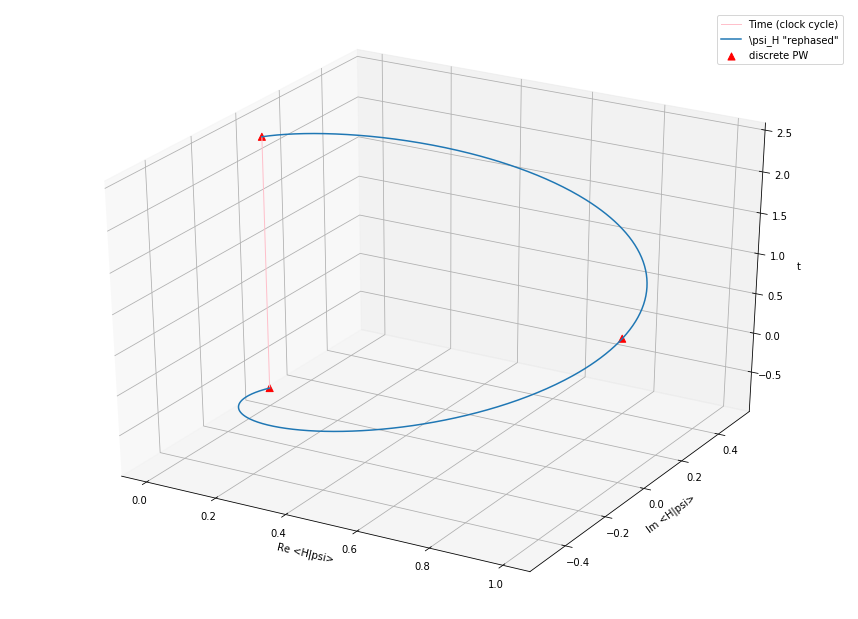
\includegraphics[width=\textwidth]{img/psi_H.png}
  \caption{
    Evolution of $\braket{H}{\psi(t)}$ in the two models.
  }
  \label{fig:psi_H}
\end{figure}

\begin{figure}
  %\centering
  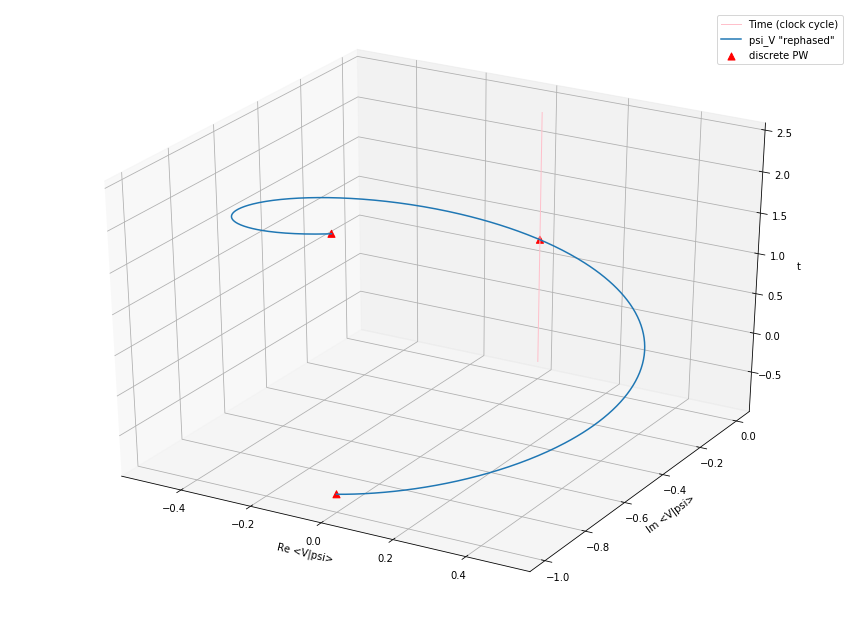
\includegraphics[width=\textwidth]{img/psi_V.png}
  \caption{Evolution of $\braket{V}{\psi(t)}$ in the two models.}
  \label{fig:psi_V}
\end{figure}
  
\if{todo}
%% CUT sections from here into other files when you DO them

\section{Absorption by a detector, time of arrival}
Ref: \cite{RuschhauptAbsorption}.

Qubit PW vs Ruschhaupt detector on 2-level system,
particularly section “EMISSION FROM A TWO-LEVEL SYSTEM”.

Idea: the ``deviation'' from continuity equation as ``absorption event'',
normalizable in $L^2(\mathbb{R}^4)$.

\section{Quantum computing, IBM, decomposition, Trotter-SUzuki, Sine-cosine, qubiter dir}

Previous section(s) read(s):
\begin{quote}
  A benefit of finite-dimensional systems is the potential implementation on a finite array of
  qubits in a quantum computer.
\end{quote}
Make a ref from there to here, and talk about qubiter and stuff.

Also, \cite{Moreva:illustration} has FIG.1 gate array repr\dots

\section{Prvanovic and P\&W}
In \cite{Prvanovic}, essentially the clock observable is the Hamiltonian.
The two example clocks are an harmonic oscillator and a free particle.
The harmonic oscillator features discrete time. Generally a time which is
{bounded from below}
is consistent with the Big Bang...

Prvanovic uses ``relativisitc'' constants...

\section{Entanglement and decoherence (Arrow of time)}
See also \cite{EntanglementVsDecoherence}.

Decoherence is an irreversible process, it also happens in measurement.

According to Marletto and Vedral, arrow of time is increase in Entanglement
between the clock and the rest.

So, there seems to be a contradiction: is entanglement ``decreasing''
(i.e. destroyed by decoherence) with time
or increasing?

We can avoid the contradiction saying that
entanglement between two finite systems is
destroyed while the entanglement of each of them with the universe
is increasing.

\section{TODOs}

TODO: \cite{Lloyd:Time} does not only deal with improper eigenstates in $\hilb{H}_T$
(full evolutions?)
but also normalized ones (in $\hilb{H}_T$! \emph{``Events''}?)

TODO: \cite{RealisticClocks}.

\cite{HarmonicClocks} concludes ``Classical clock can be described by an Hamiltonian linear in momentum''\dots
like in relativity?

Extra: \cite{TimeAnyons}.

TODO: use the harmonic oscillator in \cite{HarmonicClocks}
as a PaW clock for the same packet that is measured in
Ruschhaupt's detector model.

Therein, fading wave function: is minus derivative an event?
L4 normalized?

Other systems of interest: decays. Prvanovic new.

TQM Book: time of residence: applicable to qubits, therefore Moreva experiment.

\url{https://arxiv.org/abs/1708.04302} majorization, thermo.

\section{and paths}

Both \cite{YearsleyHalliwell_Clocks} and \cite{Gambini_PW}
reason in terms of paths and actions, maybe Feynmann stuff
in following chapter... and maybe conistent historiesapproach can help
towards linking PaW and ToA?

Also \url{http://quantum.phys.cmu.edu/CHS/CHS_transp.pdf}.

\section{and dwell time}

\cite[\S 5]{TQM2}, \cite{YearsleyHalliwell_Clocks}.

\section{In relation with the \term{time of residence}}

Here we compare \cite{Moreva:synthetic, Moreva:illustration}
(a Page and Wootters problem)
with the ``standard'' \term{time of residence}
treated in \cite[\S 5.5.2]{TQM2},
the only usable concept since there is no notion of position
for a qubit.

\section{Comparison with (Kijowski/Aharonov-Bohm) time of arrival}

Time of arrival is derived for non-relativistic \parencite{Delgado_TOA, Delgado_TOA2}
and relativisitic \parencite{Leon_TOA_R}
particle.

Kijowski: \cite{Kijowski_Time, Kijowski_Comment}.

A Page and Wootters time of arrival is mentioned in \cite{Gambini_PW}.

Time of arrival and clocks: again, \cite{YearsleyHalliwell_Clocks}.
Which maybe suggests we should not wory too much of $H\ket{\Psi} = 0$. 

BUT please note \cite{YearsleyHalliwell_Clocks} uses a clock that is
\emph{coupled} with the system, while in PaW they are ``only'' entangled.
So their calculation may be unnecessarily complicated.
Maybe the weakjly coupling case can be used?

\section{In relation to Leggett-Garg inequalities}
(Also mentioned in \cite{Moreva_position}).

Ref \cite{LeggettGarg+PageWootters}.

But also Lloyd: \url{https://arxiv.org/abs/1608.05672},
\emph{Decoherent histories approach to the cosmological measure problem}.
Lindbladt, Markov, Open Systems.

Halliwell, \url{https://arxiv.org/abs/1604.01659}. Ancilla, decay (spontaneous emission?).

A phylosophical object to decoherent histories / Everett (Everett mentioned in Marletto/ref)
is at
\url{https://arxiv.org/abs/1603.04845}.
\section{Detector model}

\cite{TQM2} (Kijowski and Detector) is cited and summarized well in
\cite{Halliwell_Detector}.



\section{Can a POVM on a system, if then we see it as part of a bipartite one,
equivalent to a PVM on the other, entangled, system?}

TODO: backflow effect in both models.

This will show an equivalence of models based on POVM with the Page and Wootters...?

Well, yes.

From \cite{PreskillNotes}, Ch.3 
\begin{quotation}
We have seen that
a pure state of the bipartite system AB may behave like a mixed state
when we observe subsystem A alone, and that an orthogonal measurement
of the bipartite system can realize a (nonorthogonal) POVM on A alone.
\end{quotation}

and

\begin{quotation}
A POVM in $H_A$ can be realized as a unitary transformation on the tensor
product $H_A \otimes H_B$, followed by an orthogonal measurement in $H_B$.
\end{quotation}

The same chapter talks about quantum operations, quantum channels and Kraus opertators.

We might want to look at exponential decay from \url{https://arxiv.org/abs/1704.07236},
then compare with exponential decay with P and W using Lloyd Giovannetti and Maccone (ref).

\subsection{Purification}

See https://arxiv.org/pdf/quant-ph/0512125.pdf, P-W time as a purifying ancilla
of the (Kijowski?) time.

\subsection{4-partite universe?}
\begin{itemize}
  \item{The system being measured/detected}
  \item{The Ruschhaupt detector --- which does not measure time, but whose detection happens at a certain time}
  \item{The Page and Wootters clock, entangled with the system and/or the detector}
  \item{The rest of the Universe, aka the Environment, aka the Termal Bath or Reservoir}
\end{itemize}

Can any of the above be identified? If the lab is isolated enough,
the detector is the only macro object and can act as a Universe/bath/environment/reservoir\dots?

\section{On ``taking time seriously'' (time is real) and why it can still be real in Page and Wootters}

No, Smolin
(\term{Time Reborn}, \term{The Singular Universe and the Reality of Time})
pushes this too far, even Special Relativity's time is too ``virtual'' for him.
Similarly, the philosopher Tim Maudlin

\url{https://www.quantamagazine.org/a-defense-of-the-reality-of-time-20170516/}

Here instead we just argue that the clock can actually be really time, not any observable.
We use notation $T$ as in time instead of $C$ as in clock etc.

In this sense, the Moreva experiment is a quantum analogue simulation.
\fi

\chapter{Irreversible processes}
\section{Unitary evolution, absorption, events}

A vector $\dket{\Psi}$ in $\hilb{H}_T \ox \hilb{H}_S$,
satisfying \eqref{eq:pwHamiltonian} and \eqref{eq:Wheeler-DeWitt},
encodes the whole (unitary) time evolution of a system.
\begin{equation}\label{eq:pwexpansion}
  \dket{\Psi} =
    \int \dd{t} \ket{t}_T \ox \ket{\psi(t)}_S =
    \int \dd{t}\dd[3]{\vec{r}} \ \Psi(t; \vec{r}) \; \ket{t}_T \ox \ket{\vec{r}}_S
    \,  \text{.}
\end{equation}
We know $\ket{t}_T \ox \ket{\vec{r}}_S$ is an othonormal basis of $\hilb{H}_T \ox \hilb{H}_S$, therefore
\begin{equation}
  \norm{\dket{\Psi}}^2 =
    \int \dd{t}\dd[3]{\vec{r}} \ \abs{\Psi(t; \vec{r})}^2 =
    \int \dd{t} \int \dd[3]{\vec{r}} \ \abs{\Psi(t; \vec{r})}^2 =
    \int \dd{t} 1 \rightarrow +\infty
    \,  \text{,}
\end{equation}
which means that such $\dket{\Psi}$ is an \term{improper} vector of $\hilb{H}_T \ox \hilb{H}_S$.

Proper (i.e. normalizable) states are described in \cite{Lloyd:Time} as well, by replacing (or generalizing)
the \eqref{eq:pwexpansion} with
\begin{equation}\label{eq:pwphi}
  \dket{\Psi} =
    \int \dd{t} \phi(t) \ket{t}_T \ox \ket{\psi(t)}_S \, \text{.}
\end{equation}
If the function $\phi \in \mathcal{L}^2(\mathbb{R})$,
then $\dket{\Psi}$ is a proper element of the product space,
and $\norm{\dket{\Psi}}^2 = \int \dd{t} \abs{\phi(t)}^2$.

We will consider some even more general case than \cite{Lloyd:Time},
for example when $\phi(t)$ is not a constant, but it's not square-integrable either,
or it's such only in the half-line $\mathbb{R}^{+}$,
which will be useful in some problems.

The case of non-normalizable $\dket{\Psi}$ in \eqref{eq:pwphi},
with normalized $\ket{\psi(t)}_S$ $\forall t \in \mathbb{R}$,
describes the unitary evolution, as seen throughout Chapter \ref{ch:pw}.
As observed in \cite{Maccone:QGR},
``%
  Quantum mechanics is formulated in terms of \emph{systems},
  typically limited in space but infinitely extended in time%
''.
If the state vector is \emph{conditioned} at a particular time $t$,
it holds $\norm{_{T}\bradket{t}{\Psi}}_S = \norm{\ket{\psi(t)}}_S = 1$,
meaning that, at each $t$,
\emph{the particle must certainly be in some (one) point in space}.

A normalized $\dket{\Psi}$ in the whole $\hilb{H}_T \ox \hilb{H}_S$,
instead,
can be interpreted as a total probability of~$1$ in both space and time combined.
It's an \term{event} that, as such, must certainly be in some point in space
\emph{and} at some individual time (in terms of outcome of an idealized measurement).
A ``typical'' example of localized ``event wave packet'' would be
therefore represented by
a \emph{4-dimensional} gaussian wave function,
in analogy to well known examples of purely spatial gaussian states
in quantum mechanics and quantum optics.

As an intermediate case, we may want to consider e.g.
$\phi(t) = 1$ for $t < 0 $ and a definitive decreasing behavior
in the positive half-line with $\lim_{t \to +\infty} \phi(t) = 0$.
In terms of ``spatial quantum mechanics'', we will compare this case with
models of detection by absoption \parencite{RuschhauptAbsorption},
where the evolution is not unitary and
the norm of $\ket{\psi(t)}$ vanishing with $t \to +\infty$
as a consequence of a \term{complex potential}
i.e.
an Hamiltonian corrected by a an anti-hermitian term
that models the detector.

A non hermitian Hamiltonian is justified as a computation method
to simplify the study of some open systems: the evolution of mixed
states is derived without explicit reference to density operators
or master equations, but resolving equations that are formally
identical to those of pure states,
i.e. in terms of
Schr{\"o}dinger equations and wave functions,
with the non-hermitian term in the Hamiltonian
to account for the non-unitarity of the evolution
(\cite[Ch. 6]{TQM2}; \cite{Wave-function_approach}; \cite{HowToResetAnAtom}; \cite{TheQuantumJumpApproach}).

\section{Detection, absoption and complex potentials}

Quantum Jumps / trajectories / Monte Carlo Wave Function.

Ch. 6 Vol. 2 of Time in QM (G.C. Hegerfeldt). Or similarly
\begin{itemize}
  \item \url{https://arxiv.org/pdf/quant-ph/9710027.pdf}
  \item Gerhard C Hegerfeldt and Dirk G Sondermann 1996 Quantum Semiclass. Opt. 8 121
  \item  Almut Beige et al 1996 Quantum Semiclass. Opt. 8 999
  \item VOLUME
  \item 68,NUMBER 5 PRL 1992 Wave-Function Approach to Dissipative Processes in Quantum Optics
  \item ``How to reset an atom after photon detection'' 
  \item BEST: \url{http://www.theorie.physik.uni-goettingen.de/~hegerf/trieste.pdf}
  \item OR: textbooks and monographs: Carmichael, Scully, Milburn, Gerry
\end{itemize}

Qubit PW vs Ruschhaupt detector on 2-level system,
particularly section “EMISSION FROM A TWO-LEVEL SYSTEM”.

Idea: use section B ``Measurement'' of \cite{Lloyd:Time}: detector as (binary) measument device.

Idea: the ``deviation'' from continuity equation as ``absorption event'',
normalizable in $L^2(\mathbb{R}^4)$.

\cite{TQM2} (Kijowski and Detector) is cited and summarized well in
\cite{Halliwell_Detector}.

``Philospher'': \url{https://arxiv.org/abs/1704.07236}.

\subsection{Use open quantum systems theory in ``Decoherence and measurement'' chapter}
Schmidt decompositions, spatial and temporal states in
$\hilb{H}_T$ and $\hilb{H}_S$
are described as density operators
(mixed states). What if there isn't a ``perfect entanglment'' between space and time.

\section{Non-unitary dynamics in $\hilb{H}_S$, in Page-Wootters terms}

First of all,
when the unproper vector of $\hilb{H}_T \ox \hilb{H}_S$
\begin{equation}
  \dket{\Psi} = \int dt \ket{t}_{T} \ox \ket{\psi(t)}_{S}
\end{equation}
is replaced by a \emph{proper}, normalized $\dket{\Phi}$ (eq. \ref{eq:pwphi}),
what should the equation
\begin{equation}\label{eq:pwwd}
  \qty(\hbar\hat{\Omega} \ox \idop_S + \idop_T \ox \hat{H}_S)\dket{\Psi} = 0
\end{equation}
be replaced with?

As $\setof{\ket{t}_T}$ is an eigenbasis of $\hat{T}$, the \eqref{eq:pwphi}
contains the definition of an operator function in $\hilb{H}_T$,
and can then be reformulated as:\footnote{
  Or, more precisely, $\dket{\Psi} = \qty( \phi(\hat{T}) \ox \idop_S ) \dket{\Psi}$,
  but we will omit, in some cases,
  tensor product by identity operators
  when it's obvious.
}
\begin{equation}
  \dket{\Phi} = \phi(\hat{T})\dket{\Psi} \, \text{.}
\end{equation}

We will also need the relation
\begin{equation}\label{eq:fcomm}
  \comm{\phi(\hat{T})}{\hat{\Omega}} = \dot{\phi}(\hat{T}) \comm{\hat{T}}{\hat{\Omega}}, \,
    \forall \, \hat{T}, \hat{\Omega} \text{ self-adjoint in } \hilb{H}_T \text{ and } \phi \in C^{\infty}(\mathbb{R}) \, \text{,} 
\end{equation}
where $\dot{\phi}$ is the first derivative of the function $\phi$.
In fact, this is proven in Appendix \ref{CommProp} for when $\phi$ is a polynomial,
and the proof can be easily extended to a more general case by series expansion.
For the canonical pair, this will just reduce to $\comm{\phi(\hat{T})}{\hat{\Omega}} = i \dot{\phi} (\hat{T})$.

Therefore:
\begin{multline}\label{eq:complex_dynam_deriv}
  \qty( \hbar\hat{\Omega} \ox \idop_S + \idop_T \ox \hat{H}_S ) \dket{\Phi} =
  \hat{\mathbb{J}}\dket{\Phi} =
  \hat{\mathbb{J}} \qty( \phi(\hat{T}) \ox \idop_S) \dket{\Psi} =
  \\
  \qty( \hbar\hat{\Omega}\phi(\hat{T}) \ox \idop_S + \phi(\hat{T}) \ox \hat{H}_S )\dket{\Psi} =
  \qty{
    \hbar\qty( \phi(\hat{T})\hat{\Omega} - \comm{\phi(\hat{T})}{\hat{\Omega}} ) \ox \idop_S +
    \phi(\hat{T}) \ox \hat{H}_S
  }\dket{\Psi} =
  \\
  \qty(
    \phi(\hat{T}) \ox \idop_S
  )
  \qty(
    - i \hbar \frac{\dot{\phi}}{\phi} (\hat{T}) \ox \idop_S
    + \hbar\hat{\Omega} \ox \idop_S
    + \idop_T \ox \hat{H}_S
  ) \dket{\Psi} =
  \\
  - \qty( i \hbar \frac{\dot{\phi}}{\phi} (\hat{T}) \ox \idop_S ) \dket{\Phi}
  \text{,}
\end{multline}
where we have used the \eqref{eq:pwwd} first, then the fact that $\phi(\hat{T})$ 
and $-i\hbar\frac{\dot{\phi}}{\phi}(\hat{T})$ commute.

Comparing the first and last term of \eqref{eq:complex_dynam_deriv} we have:
\begin{equation}\label{eq:nonu_pwwdw}
  \qty[
    \hbar\hat{\Omega} \ox \idop_S +
    i \hbar \frac{\dot{\phi}}{\phi}(\hat{T}) \ox \idop_S +
    \idop_T \ox \hat{H}_S
   ] \dket{\Phi} = 0
  \text{,}
\end{equation}
showing that a non-hermitian\footnote{
  Unless $\phi$  is a pure imaginary function.
}
term
$i \hbar \frac{\dot{\phi}}{\phi} (\hat{T})$
emerges as a correction to the dynamic constraint $\hat{\mathbb{J}}$.
In fact, the \eqref{eq:complex_dynam_deriv}
is a more detailed proof of what stated in
\cite[eq. 27]{Lloyd:Time}.

It's worth remarking that the \eqref{eq:complex_dynam_deriv} does not really require
$\phi \in \mathcal{L}^2(\mathbb{R})$, therefore the last result does not only apply
to normalized vectors as in \eqref{eq:pwphi}, but can apply to cases like
\eqref{eq:pwf}, provided that regularity conditions are met such that
the \eqref{eq:fcomm} is satisfied.
\begin{equation}\label{eq:nonu_pwwdw_f}
  \qty[
    \hbar\hat{\Omega} \ox \idop_S +
    i \hbar \frac{\dot{f}}{f}(\hat{T}) \ox \idop_S +
    \idop_T \ox \hat{H}_S
   ] \dket{\mathsf{F}} = 0
  \text{,}
\end{equation}
This gives validity,
under such regularity conditions,
to a comparison
between 
this \term{Page-Wootters} result,
and absorption detector models
as recalled in \cite{RuschhauptAbsorption}.
\section{Comparison with detector absorption models}

By ``conditioning'' the \eqref{eq:nonu_pwwdw} at each time $t$
---in other words: by inner-multiplying it on the left with the partial bra\footnote{
  Partial in the sense of open quantum systems
  i.e. as a part of a bipartite system.
  See Definition \ref{def:pBra}.
}
$\prescript{}{T}{\bra{t}}$~---
a modified Schr{\"o}dinger equation
can be derived,
as a variant of \eqref{eq:schrod_from_pw}.

In the position representation of $\hilb{H}_S$ (and ``tracing out'' time):
\begin{equation}\label{eq:schrod_pw_nonunitary}
  \hat{H} \ket{\phi(t)} = i\hbar\dv{t}\ket{\phi(t)} -i\hbar\frac{\dv{\phi}{t}}{\phi(t)}\ket{\phi(t)} \text{.}
\end{equation}

Here the subscript $S$ has been removed and it's assumed.
$\ket{\phi(t)} = \prescript{}{T}{\bradket{t}{\Phi}}$
is a state vector that does not conserve its norn in its time evolution.
In a sense, its norm is ``absorbed'' in the detection process.

Within the Page-Wootters framework, a non-hermitian term in the ``Hamiltonian''
is a consequence of non-unitary ``evolution''.
On the contrary, in detection models based on absorption and complex potentials
\parencite{RuschhauptAbsorption}, non-unitary evolution is a consequence
of such non-hermitian term in the modified Hamiltonian.
Specifically, the Hamiltonian $\hat{H}$ is replaced by a $\hat{H} - i\hat{D}$
(with $\hat{D}$ self-adjoint, bounded, positive ---\cite{RuschhauptAbsorption})
and, consequently:
\begin{equation}\label{eq:schrod_complex_pot}
  \hat{H} \ket{\phi(t)} = i\hbar\dv{t}\ket{\phi(t)} +i\hat{D}\ket{\phi(t)} \text{.}
\end{equation}
Similarly to the Page-Wootters model, $\ket{\phi(t)}$ does not conserve its norm in time.

In the P-W model, $\ket{\psi(t)} = \ket{\phi(t)}/\phi(t)$
is the corresponding unitary evolution vector
(or ``what would have happened without an absorbing detector'').
This relation, along with \eqref{eq:schrod_complex_pot} and \eqref{eq:schrod_pw_nonunitary},
yields a differential equation
\begin{equation}\label{eq:phi_diffeq}
  -\hbar\dv{\phi}{t}\ket{\psi(t)} = \phi(t) \hat{D} \ket{\psi(t)} \text{,}
\end{equation}
where $\phi(t)$ and $\hat{D}$ commute, as $\hat{D}$ only acts on the spatial degrees of freedom,
while $\phi(t)$ is, with respect to $\hilb{H}_S$, in fact a constant, albeit parametrized in $t$.

One may find $\ket{\psi(t)}$ first (by simply computing the unitary evolution),
then compute the effect of the detector by resolving the \eqref{eq:phi_diffeq}
which is then an ordinary differential equation in $\phi$. This is, of course, valid
under the assumption that the detector term only affects norm and phase,
but doesn't change the ``ray'' of the state vector in the Hilbert space. 

Multiplying on the left by $\bra{\psi(t)}$, rearranging, and with the same observations
on commutativity:
\begin{equation}\label{eq:phi_diffeq_simpler}
  -\hbar\frac{\dot{\phi}}{\phi}(t) = \ev{D(t)} \text{,}
\end{equation}
a well known equation type based on logaritmic derivative: in particular,
if $\hat{D}$ is a constant, that would bring an exponential decay law.
A general solution is:
\begin{equation}
  \phi(t) = \phi(t_0) \exp[ -\frac{1}{\hbar} \int_{t_0}^{t} \dd{t'} \ev{D(t')} ]
\end{equation}
where:
\begin{enumerate*}[label=\emph{\alph*})]
  \item
    the physics of the problem may tell us, for example, a time when $\phi(t_0) = 1$;
  \item
    a suitable interval $\qty[t_0, t]$ may be chosen where it is $\phi(t') \ne 0$
    to avoid singularities in \eqref{eq:phi_diffeq_simpler};
  \item
    again, $\ev{D(t)} = \mel{\psi(t)}{\hat{D}}{\psi(t)}$ is a known function
    once the unitarily evolved $\ket{\psi(t)}$ is determined.
\end{enumerate*}


   
\if{todo}
\section{Entanglement and decoherence (Arrow of time)}
See also \cite{EntanglementVsDecoherence}.

Decoherence is an irreversible process, it also happens in measurement.

According to Marletto and Vedral, arrow of time is increase in Entanglement
between the clock and the rest.

So, there seems to be a contradiction: is entanglement ``decreasing''
(i.e. destroyed by decoherence) with time
or increasing?

We can avoid the contradiction saying that
entanglement between two finite systems is
destroyed while the entanglement of each of them with the universe
is increasing.




\section{``Harmonic clocks''}

TODO: use the harmonic oscillator in \cite{HarmonicClocks}
as a PaW clock for the same packet that is measured in
Ruschhaupt's detector model.

Therein, fading wave function: is minus derivative an event?
L4 normalized?


\section{Misc}

Time of arrival and clocks: again, \cite{YearsleyHalliwell_Clocks}.
Which maybe suggests we should not wory too much of $H\ket{\Psi} = 0$. 

We don't. 

BUT please note \cite{YearsleyHalliwell_Clocks} uses a clock that is
\emph{coupled} with the system, while in PaW they are ``only'' entangled.
So their calculation may be unnecessarily complicated.
Maybe the weakjly coupling case can be used?

Other systems of interest: decays. Prvanovic new.

Reference \cite{ConnesRovelliThermo}.

Relate with John Goold's works? The ancilla as a clock? --- Topical Review

Markovianity, histories.

Lloyd on arXiv: from clock to cloners; erasing; scrambling (as in Goold).

Lloyd on decoherent histories (Gellman, Hartle?).

Dechoerence / irreversibility / measurement.

Vedral / Lloyd. Discord.

Measuring entanglement: Quantification of Concurrence via Weak Measurement: 1611.00149.

Marletto/Vedral on Arrow of time. Arrow of time as increasing entanglement.

Arrow of time: 

\url{https://www.wired.com/2014/04/quantum-theory-flow-time/}

\url{https://en.wikipedia.org/wiki/Loschmidt%27s_paradox}

\url{https://www.quantamagazine.org/20160119-time-entanglement/}

\url{https://arxiv.org/pdf/1702.07706.pdf} \textit{The second law of thermodynamics at the microscopic scale}
Thibaut Josset,
Aix Marseille Univ. (David).

Maxwell's demon: https://arxiv.org/pdf/1702.05161.pdf

\subsection{and paths}

Both \cite{YearsleyHalliwell_Clocks} and \cite{Gambini_PW}
reason in terms of paths and actions, maybe Feynmann stuff
in following chapter... and maybe conistent historiesapproach can help
towards linking PaW and ToA?

Also \url{http://quantum.phys.cmu.edu/CHS/CHS_transp.pdf}.

\subsection{Can a POVM on a system, if then we see it as part of a bipartite one,
equivalent to a PVM on the other, entangled, system?}

TODO: backflow effect in both models.

This will show an equivalence of models based on POVM with the Page and Wootters...?

Well, yes.

From \cite{PreskillNotes}, Ch.3 
\begin{quotation}
We have seen that
a pure state of the bipartite system AB may behave like a mixed state
when we observe subsystem A alone, and that an orthogonal measurement
of the bipartite system can realize a (nonorthogonal) POVM on A alone.
\end{quotation}

and

\begin{quotation}
A POVM in $H_A$ can be realized as a unitary transformation on the tensor
product $H_A \otimes H_B$, followed by an orthogonal measurement in $H_B$.
\end{quotation}

The same chapter talks about quantum operations, quantum channels and Kraus opertators.

We might want to look at exponential decay from \url{https://arxiv.org/abs/1704.07236},
then compare with exponential decay with P and W using Lloyd Giovannetti and Maccone (ref).

\subsubsection{Purification}

See https://arxiv.org/pdf/quant-ph/0512125.pdf, P-W time as a purifying ancilla
of the (Kijowski?) time.

\subsubsection{4-partite universe?}
\begin{itemize}
  \item{The system being measured/detected}
  \item{The Ruschhaupt detector --- which does not measure time, but whose detection happens at a certain time}
  \item{The Page and Wootters clock, entangled with the system and/or the detector}
  \item{The rest of the Universe, aka the Environment, aka the Termal Bath or Reservoir}
\end{itemize}

Can any of the above be identified? If the lab is isolated enough,
the detector is the only macro object and can act as a Universe/bath/environment/reservoir\dots?

\fi

\chapter{Relativistic treatment}
\section{Relativistic formulation: Klein-Gordon}

The Klein-Gordon equation is the relativistic extension of the
(\emph{square of}) a wave equation for a free spinless particle.
Indeed, both sides have the dimension of
the square of an energy, and finding their square root
(in the operator sense) is non trivial task which was only resolved 
with the Dirac equation, from which the
intrinsic \term{spin} (particularly spin $\hbar/2$) logically emerges,
rather then being artificially introduced in the theory
to comply with the phenomenology
(\cite{Greiner_Rel}, \cite[Ch. 8]{Sakurai2}, \cite{DiracEquation}, \cite[handout 2]{Webber_notes}).

Both equations did not have much fortune as first-quantized equations,
for conceptual difficulties and historical reasons, including the rise
of Quantum Field Theory and second quantization. They do have a fundamental
role though as field equations (before quantization methods are enacted).
\parencite{PeskinSchroeder}.

The purpose of the present work is, in a sense, promoting time to a quantum
observable, or formally to a linear, self-adjoint operator in some Hilbert space.
The passage from quantum mechanics to field theory does not represent any progress
towards such goal, in that not only it does not ``promote'' time to an operator $\hat{t}$,
but it also ``demotes'' the three position operators $\hat{x}$, $\hat{y}$ and $\hat{z}$
to mere (classical) \emph{parameters}. However, consistently to relativistic covariance,
time and space coordinates are treated on equal footing. The Page and Wootters model
offers the opportunity to do the same, but both time and position are operators!

\subsection{Page and Wootters squared}

From the \eqref{eq:pwHamiltonian} and \eqref{eq:Wheeler-DeWitt}:
\begin{equation}\label{eq:pw_to_be_squared}
  -\hbar\hat{\Omega}\ox\idop_S \dket{\Psi} = \idop_T\ox\hat{H}_S \dket{\Psi} \,\text{.}
\end{equation}
Squaring the operators on both sides, we have:
\begin{equation}\label{eq:pw_squared}
  \hbar^{2}\hat{\Omega}^{2}\ox\idop_S \, \dket{\Psi} = \idop_T\ox\hat{H}_S^{2} \,\, \dket{\Psi} 
    = \idop_T \ox \left( \hat{p}^2 c^2 + m_0^2 c^4 \right) \dket{\Psi} \,\text{,}
\end{equation}
where the last equality is due to the ``quantization'' of the relation $E^2 = p^2 c^2 + m_0^2 c^4$
into $\hat{H}_S^{2} = \hat{p}^2 c^2 + m_0^2 c^4$.

We know from previous sections that in the $\qty{\ket{t}}_T$ basis $\hat{\Omega}$ is represented as
$-i\hbar\pdv{t}$. We know from standard quantum mechanics that in the $\qty{\ket{x}\ket{y}\ket{z}}_S$
basis is $\hat{p} \repr -i\hbar\nabla$. Therefore in the product basis the \eqref{eq:pw_squared} yields:
\begin{equation}\label{eq:proto_kg}
  -\hbar^2\pdv[2]{t}\Psi = \qty(-\hbar^2 c^2 \nabla^2 + m_0^2 c^4)\Psi
\end{equation}
which, up to some elementary algebra, is the well known \term{Klein-Gordon equation}.

In standard quantum mechanics (first quantization, relativistic or not)
\begin{equation}
  \ket{\psi(t)} = \int \dd{x}\dd{y}\dd{z} \Psi(x,y,z;t) \ket{x}\ox\ket{y}\ox\ket{z} \,\text{.}
\end{equation}
In this formulation
\begin{equation}
  \dket{\Psi} = \int \dd{x}\dd{y}\dd{z}\dd{t} \Psi(x,y,z,t) \ket{x}\ox\ket{y}\ox\ket{z}\ox\ket{t} \,\text{,}
\end{equation}
and $t$ is no longer a classical parameter, but an eigenvalue of the time operator,
or a label for time basis elements. Please note that, as a function of four variables,
$\Psi$ is not normalizable i.e. it's not a proper element of
$\mathcal{L}^2(\mathbb{R}^4)$
(normalization issues are tackled in \cite[eq. 23 and following]{Lloyd:Time}).

\subsection{Covariant notation}

The \eqref{eq:proto_kg} can be rearranged and expressed in explicitly covariant form:
\begin{equation}
  \qty[\partial_{\mu}\partial^{\mu} + \qty(\frac{mc}{\hbar})^2]\Psi = 0
\end{equation}
with standard relativistic notation.
Similarly
---at operator level, in the tensor product space---
the \eqref{eq:pw_squared} can be rearranged:
\begin{equation}\label{eq:pwkg}
  \qty[- \hat{\mathrm{P}}_{\mu} \hat{\mathrm{P}}^{\mu} + \qty(\frac{mc}{\hbar})^2]\Psi = 0
\end{equation}
with
\begin{equation}
\begin{aligned}\label{eq:p0123}
  \hat{\mathrm{P}}_0 &=& \frac{\hbar\hat{\Omega}}{c}  \ox \idop_x   \ox \idop_y   \ox \idop_z \\
  \hat{\mathrm{P}}_1 &=& \idop_T                      \ox \hat{p}_x \ox \idop_y   \ox \idop_z \\
  \hat{\mathrm{P}}_2 &=& \idop_T                      \ox \idop_x   \ox \hat{p}_y \ox \idop_z \\
  \hat{\mathrm{P}}_3 &=& \idop_T                      \ox \idop_x   \ox \idop_y   \ox \hat{p}_z
\end{aligned}
\end{equation}
and the usual relation between contravariant and covariant 4-vectors:
\begin{equation}
  a_\mu = \eta_{\nu}^{\mu} a^{\nu} \text{;} \quad
  \eta = \mathrm{diag}(+1, -1, -1, -1)
  \text{.}
\end{equation}

It's tempting to name the \eqref{eq:pwkg} and \eqref{eq:p0123} the \term{Page-Wootters-Klein-Gordon}
equation.\footnote{
  Or \term{Klein-Gordon-Wheeler-DeWitt-Page-Wootters-Giovannetti-Lloyd-Maccone}
  equation, thus giving
  credits to all authors, particularly if we consider that the idea of an extra Hilbert space
  was conceived originally in \cite{Lloyd:Time}.
}

As anticipated, this resolves the asymmetry in Tables \ref{op_comparison_alg} and \ref{op_comparison_J},
whereas we can write
{
  \begin{table}[h!]
    \centering
    \begin{tabular}{p{0.3\linewidth}||c|c|c}
                                                                                &
        $\hilb{H}_T$                                                            &
        $\hilb{H}_S$                                                            &
        {\footnotesize Mass term}                                               \\
      \hline
      \hline
        {\footnotesize Spatio-temporal ``positions''}                           &
        $\hat{t}$                                                               &
        $\hat{x}$                                                               &
                                                                                \\
      \hline
        {\footnotesize Canonically conjugate}                                   &
        $\hat{P_0} = \frac{\hbar\hat{\Omega}}{c} \repr -i\partial_{0}$          &
        $\hat{P}_{1,2,3} \repr -i\nabla$                                        &
                                                                                \\
      \hline
        {\footnotesize Dynamics (terms in the Wheeler-DeWitt equation)}         &
        $\hat{P}_{0}\hat{P}^{0} \repr -\hbar^2 \partial_{0}\partial^{0}$        &
        $\hat{P}_{j}\hat{P}^{j} \repr -\hbar^2 \partial_{j}\partial^{j}$        &
        $\qty(\frac{mc}{\hbar})^2$
    \end{tabular}
    \caption{
      Operators in the space-time Hilbert spaces.
    }
  \end{table}
}
\if{todo}
\section{TODOs}

TODO: \cite{RealisticClocks}.

\cite{HarmonicClocks} concludes ``Classical clock can be described by an Hamiltonian linear in momentum''\dots
like in relativity?

TODO: \cite{Lloyd:Time} does not only deal with improper eigenstates in $\hilb{H}_T$
(full evolutions?)
but also normalized ones (in $\hilb{H}_T$! \emph{``Events''}?)

A Page and Wootters time of arrival is mentioned in \cite{Gambini_PW}.

\subsection{Time-of-arrival for a Klein-Gordon free particle}

See \cite{Galapon_KG}.

\subsection{Feynmann path stuff}

Sokolovski 1703.01966, Feynmann paths...\subsection{(dis)entanglement under gravity, decoherence, event formalism}

1703.08036 An experiment to test decoherence under gravity aka entangled photons undergoing different paths and how their entanglement is affected.
``Space QUEST mission proposal: Experimentally testing decoherence due to gravity''.

Are they getting entangled with the environment instead? (Merletto and Vedral).

The theoretical paper behind the space experiment: \url{https://arxiv.org/pdf/1406.3677.pdf}. Interestingly, it mentions 
\emph{event formalism}, and we thought about that: is an event something
representable as a proper vector in $\mathcal{L}^2(\mathbb{R}^4)$ --- where one of the dimensions is time?
TODO: deepen the event formalism if it's quantum.

Resume ``Quantum Statistical Gravity''? \url{https://arxiv.org/abs/1602.05707}.

``Fundamental decoherence from quantum gravity: a pedagogical review''
\url{https://arxiv.org/abs/gr-qc/0603090} ---
``fundamental loss of unitarity
that appears in quantum mechanics
due to the use of a physical apparatus to measure time''.

Closed timelike curves are also the subject of a paper by Lloyd (cite!).

``Deutsch argued that
the usual paradoxes associated with such solutions of general
relativity can be resolved by quantum mechanics''  in the reference above. But in the even formalism
\emph{spacetime is still a classical background!}. Event operators a parametrized by $t$\dots

\subsection{Prvanovic and P\&W}
In \cite{Prvanovic}, essentially the clock observable is the Hamiltonian.
The two example clocks are an harmonic oscillator and a free particle.
The harmonic oscillator features discrete time. Generally a time which is
{bounded from below}
is consistent with the Big Bang...

Prvanovic uses ``relativisitc'' constants...




\fi

\if{todo}
\chapter{Misc \& Outlook}
\section{An intro chap on motivation and experiments?}
\begin{itemize}
  \item Time crystals?
  \item Time-resolved diffraction patters, temporal double slit experiment + Muga theory \url{https://arxiv.org/pdf/0812.3034.pdfß}
\end{itemize}

%\clearpage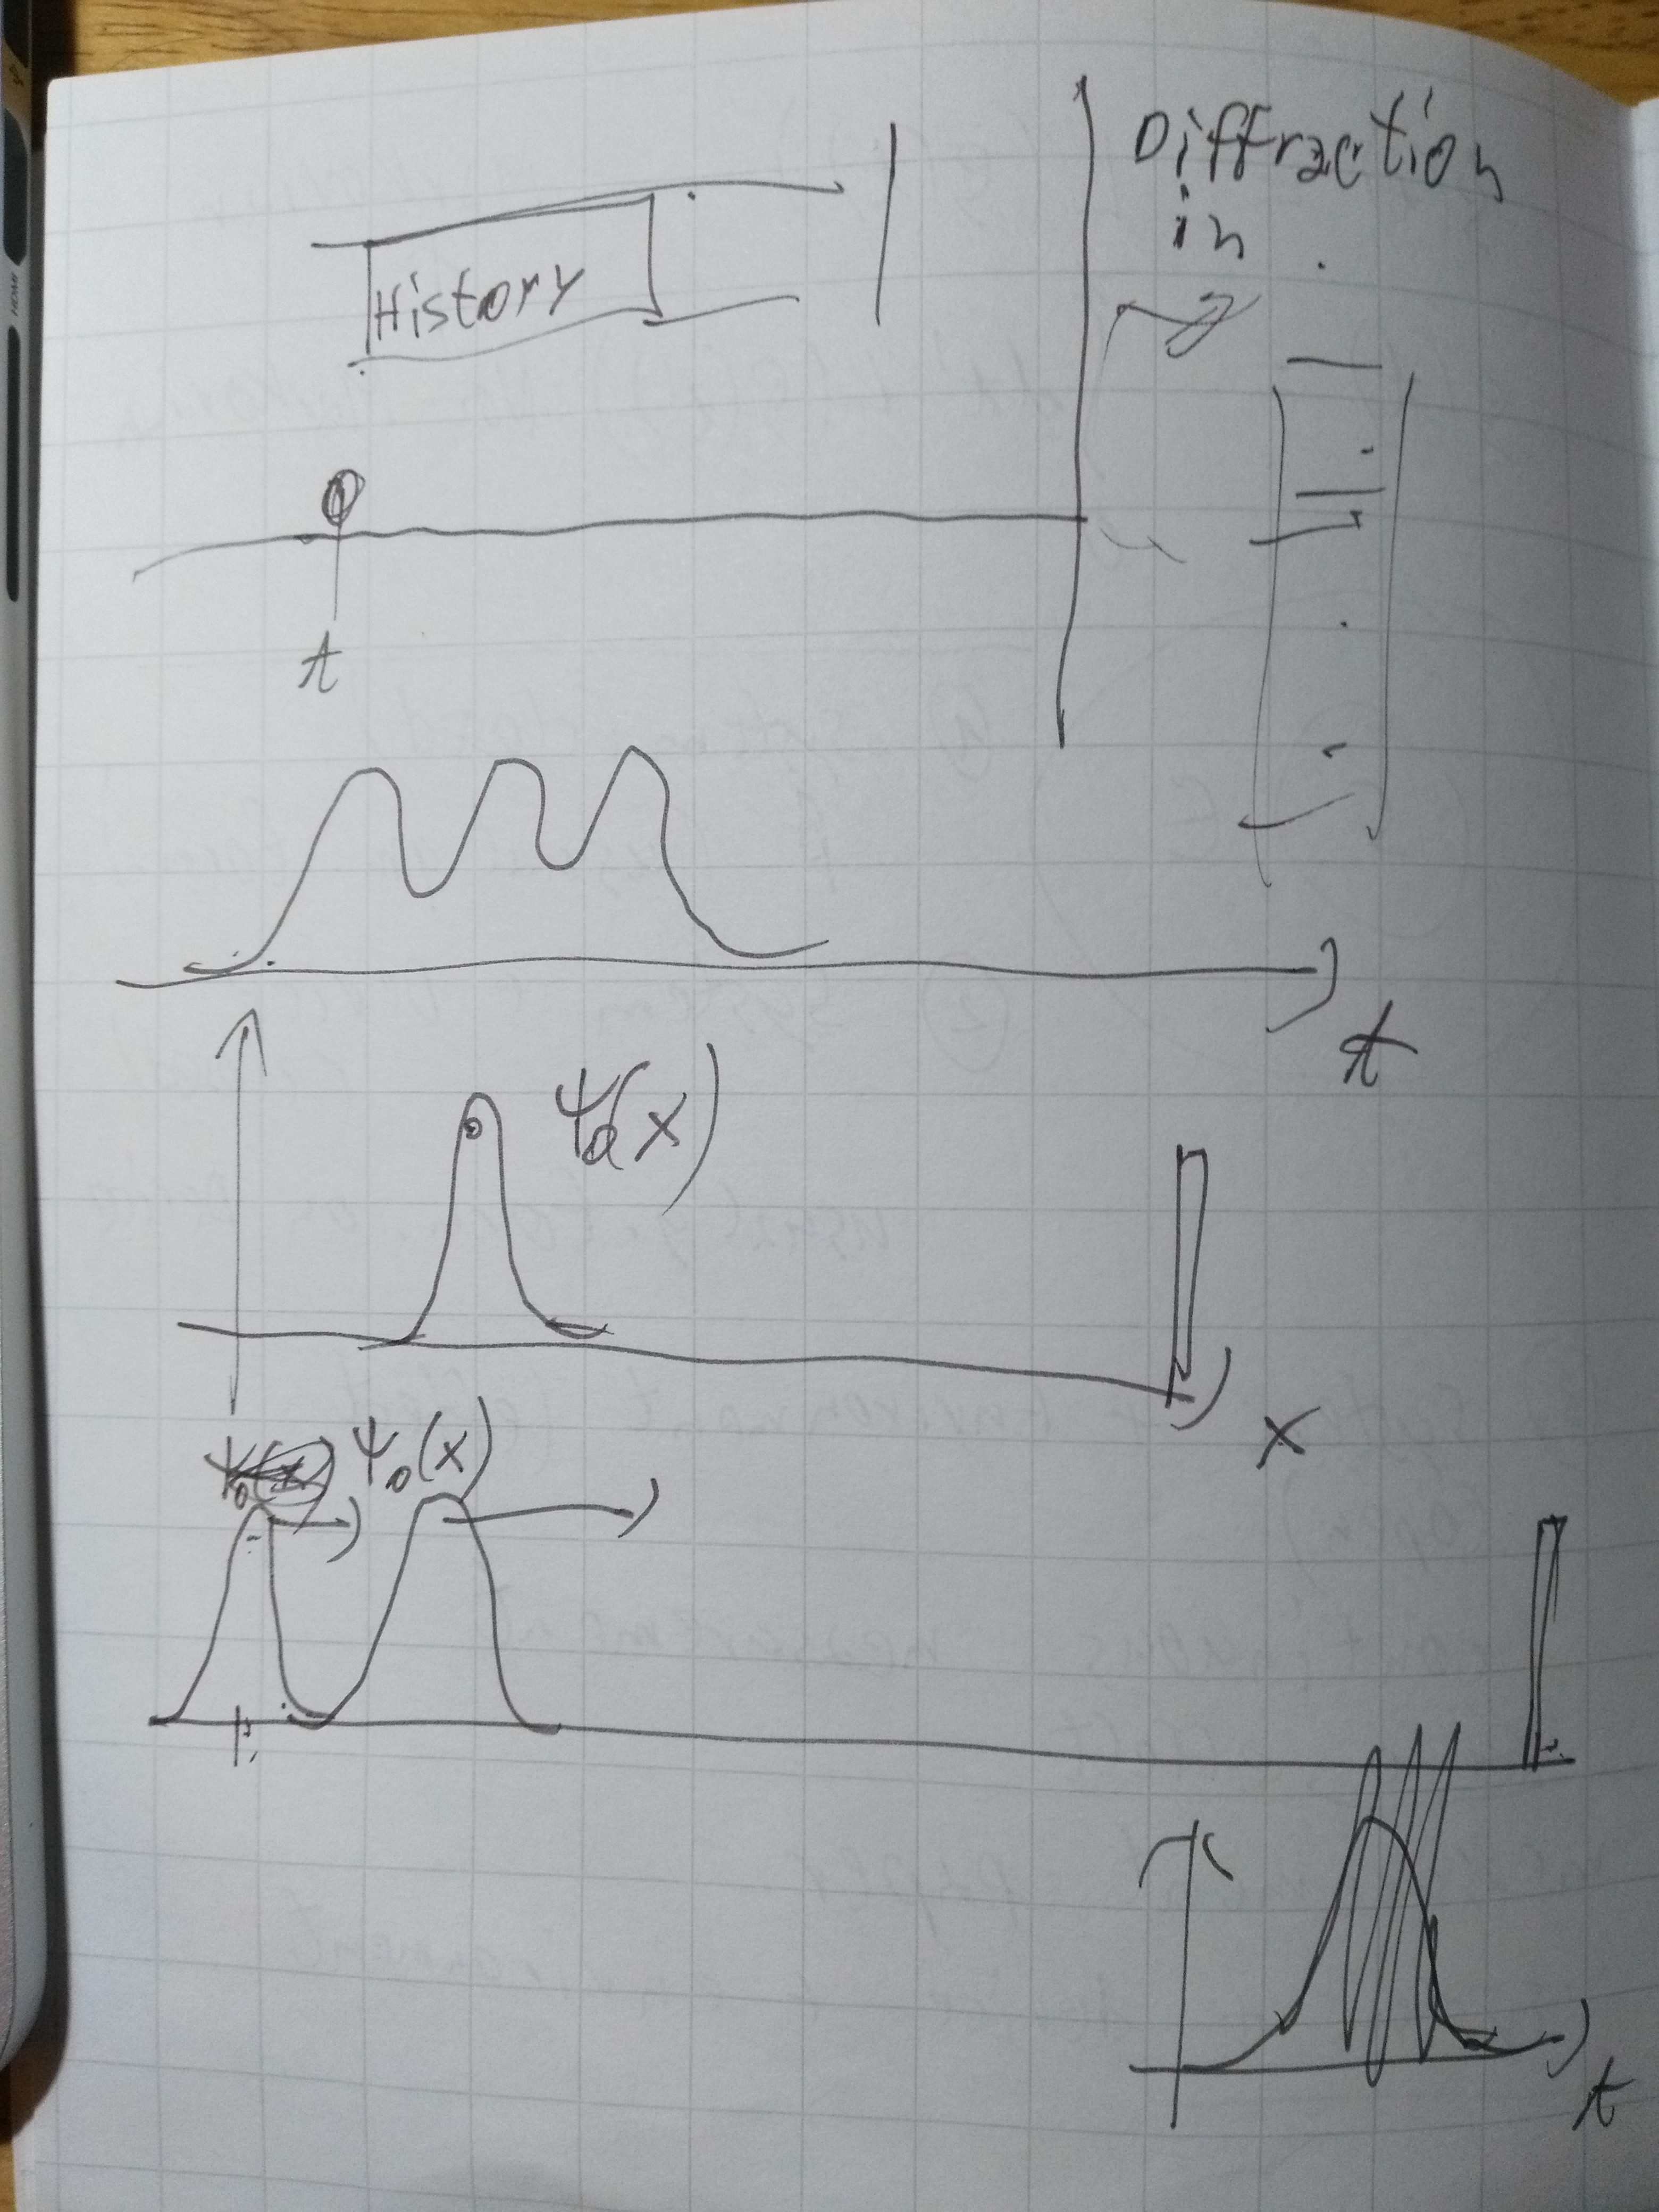
\includegraphics[width=\linewidth]{img/diffraction.jpg}

\section{pw}

Lloyd recent on entropic uncertainty (for time\dots).
From state vectors to density matrices and/or mixed states: Von Neumann entroy (wikipedia).
Subadditivity. 

\section{Misc}

\subsection{Quantum computing, IBM, decomposition, Trotter-SUzuki, Sine-cosine, qubiter dir}

Previous section(s) read(s):
\begin{quote}
  A benefit of finite-dimensional systems is the potential implementation on a finite array of
  qubits in a quantum computer.
\end{quote}
Make a ref from there to here, and talk about qubiter and stuff.

Also, \cite{Moreva:illustration} has FIG.1 gate array repr\dots

\subsection{Quantum Blockchain and Entanglement in Time}

\url{https://spectrum.ieee.org/tech-talk/computing/networks/quantum-blockchains-could-act-like-time-machines}
\url{https://arxiv.org/abs/1804.05979}


\subsection{Misc}

Extra: \cite{TimeAnyons}.

TQM Book: time of residence: applicable to qubits, therefore Moreva experiment.

\url{https://arxiv.org/abs/1708.04302} majorization, thermo.


\subsection{and dwell time}

\cite[\S 5]{TQM2}, \cite{YearsleyHalliwell_Clocks}.

\subsection{In relation with the \term{time of residence}}

Here we compare \cite{Moreva:synthetic, Moreva:illustration}
(a Page and Wootters problem)
with the ``standard'' \term{time of residence}
treated in \cite[\S 5.5.2]{TQM2},
the only usable concept since there is no notion of position
for a qubit.

\subsection{Comparison with (Kijowski/Aharonov-Bohm) time of arrival}

Time of arrival is derived for non-relativistic \parencite{Delgado_TOA, Delgado_TOA2}
and relativisitic \parencite{Leon_TOA_R}
particle.

Kijowski: \cite{Kijowski_Time, Kijowski_Comment}.

\subsection{In relation to Leggett-Garg inequalities}
(Also mentioned in \cite{Moreva_position}).

Ref \cite{LeggettGarg+PageWootters}.

But also Lloyd: \url{https://arxiv.org/abs/1608.05672},
\emph{Decoherent histories approach to the cosmological measure problem}.
Lindbladt, Markov, Open Systems.

Halliwell, \url{https://arxiv.org/abs/1604.01659}. Ancilla, decay (spontaneous emission?).

A phylosophical object to decoherent histories / Everett (Everett mentioned in Marletto/ref)
is at
\url{https://arxiv.org/abs/1603.04845}.



\subsection{On ``taking time seriously'' (time is real) and why it can still be real in Page and Wootters}

No, Smolin
(\term{Time Reborn}, \term{The Singular Universe and the Reality of Time})
pushes this too far, even Special Relativity's time is too ``virtual'' for him.
Similarly, the philosopher Tim Maudlin

\url{https://www.quantamagazine.org/a-defense-of-the-reality-of-time-20170516/}

Here instead we just argue that the clock can actually be really time, not any observable.
We use notation $T$ as in time instead of $C$ as in clock etc.

In this sense, the Moreva experiment is a quantum analogue simulation.


\section{Time crystals}

References: \cite{crystal2,crystal3,crystal2012}.


\section{Irrev}

\cite{Maccone:Pauli} \S IV.  UNBOUNDED-ENERGY CLOCKS?

\subsection{Use open quantum systems theory in ``Decoherence and measurement'' chapter}
Schmidt decompositions, spatial and temporal states in
$\hilb{H}_T$ and $\hilb{H}_S$
are described as density operators
(mixed states). What if there isn't a ``perfect entanglment'' between space and time.

Use the Von Neumann entropy (or other methods) to quantify entanglement?

When the entanglement is perfect, the notion of time evolution emerges, just
like between two dimensions n space, it may or may not ``emerge'' that
$y$ ``depends'' upon $y$ for a given distribution of positions.

\section{Entanglement and decoherence (Arrow of time)}
See also \cite{EntanglementVsDecoherence}.

Decoherence is an irreversible process, it also happens in measurement.

According to Marletto and Vedral, arrow of time is increase in Entanglement
between the clock and the rest.

So, there seems to be a contradiction: is entanglement ``decreasing''
(i.e. destroyed by decoherence) with time
or increasing?

We can avoid the contradiction saying that
entanglement between two finite systems is
destroyed while the entanglement of each of them with the universe
is increasing.

\subsection{``Harmonic clocks''}

Use the harmonic oscillator in \cite{HarmonicClocks}
as a PaW clock for the same packet that is measured in
Ruschhaupt's detector model.

Therein, fading wave function: is minus derivative an event?
L4 normalized?


\subsection{Misc}

Idea: use section B ``Measurement'' of \cite{Lloyd:Time}: detector as (binary) measument device.

``Philospher'': \url{https://arxiv.org/abs/1704.07236}.

Time of arrival and clocks: again, \cite{YearsleyHalliwell_Clocks}.
Which maybe suggests we should not wory too much of $H\ket{\Psi} = 0$. 

We don't. 

BUT please note \cite{YearsleyHalliwell_Clocks} uses a clock that is
\emph{coupled} with the system, while in PaW they are ``only'' entangled.
So their calculation may be unnecessarily complicated.
Maybe the weakjly coupling case can be used?

Other systems of interest: decays. Prvanovic new.

Reference \cite{ConnesRovelliThermo}.

Relate with John Goold's works? The ancilla as a clock? --- Topical Review

Markovianity, histories.

Lloyd on arXiv: from clock to cloners; erasing; scrambling (as in Goold).

Lloyd on decoherent histories (Gellman, Hartle?).

Dechoerence / irreversibility / measurement.

Vedral / Lloyd. Discord.

Measuring entanglement: Quantification of Concurrence via Weak Measurement: 1611.00149.

Marletto/Vedral on Arrow of time. Arrow of time as increasing entanglement.

Arrow of time: 

\url{https://www.wired.com/2014/04/quantum-theory-flow-time/}

\url{https://en.wikipedia.org/wiki/Loschmidt%27s_paradox}

\url{https://www.quantamagazine.org/20160119-time-entanglement/}

\url{https://arxiv.org/pdf/1702.07706.pdf} \textit{The second law of thermodynamics at the microscopic scale}
Thibaut Josset,
Aix Marseille Univ. (David).

Maxwell's demon: https://arxiv.org/pdf/1702.05161.pdf

\subsection{and paths}

Both \cite{YearsleyHalliwell_Clocks} and \cite{Gambini_PW}
reason in terms of paths and actions, maybe Feynmann stuff
in following chapter... and maybe conistent historiesapproach can help
towards linking PaW and ToA?

Also \url{http://quantum.phys.cmu.edu/CHS/CHS_transp.pdf}.

\subsection{Decays?}

We might want to look at exponential decay from \url{https://arxiv.org/abs/1704.07236},
then compare with exponential decay with P and W using Lloyd Giovannetti and Maccone (ref).

\subsubsection{Purification}

See https://arxiv.org/pdf/quant-ph/0512125.pdf, P-W time as a purifying ancilla
of the (Kijowski?) time.

\section{Misc/Multi/Extras/Outlook}

\url{https://arxiv.org/abs/1703.05876}
--- \emph{comment}: time measured and stored here
may be all classical information
so this paper may or may not be relevant for the topic.

But
``prototypes of clocks based on quantum principles,
such as entanglement and squeezing''
may make this interesting again, see reference therein.
They also cite Lloyd, Giovannetti and Maccone,
but a paper quite older than \cite{Lloyd:Time}.

\url{https://arxiv.org/abs/1603.02522}
\emph{Decoherence by spontaneous emission: a single-atom analog of superradiance}.
Decoherent histories, non-markovianity, open quantum systems.

\url{https://arxiv.org/abs/1007.2615} Time travel / Quantum CTC.

Carmichael et al. \cite{CarmichaelOQS2017} (Andreas's reading)
(non-markovianity).

Non-markovian, quantum-to-classical, open systems, David,
\url{https://arxiv.org/pdf/1703.09428.pdf}.

In his works, Zurek mentions:
DeWitt, Everett, gell_Mann, hartl, Many Worlds, consistent/decoherent histories:
idea: Lagrangian over a history? Principle of least action?

Zurek: ``Reduction of the Wavepacket: How Long Does it Take?'' (arxiv),
``quantum''' time? \cite{Zurek_Einselect} also mentions
``decoherence timescale''.

Von Neumann/Shannon entropy in measurement? Mention information problems
in quantum cosmology (where a quantum time is necessary)? Etc. etc.

\section{for Relativistic treatment}

\cite{RealisticClocks}.

\cite{HarmonicClocks} concludes ``Classical clock can be described by an Hamiltonian linear in momentum''\dots
like in relativity?

\cite{Lloyd:Time} does not only deal with improper eigenstates in $\hilb{H}_T$
(full evolutions?)
but also normalized ones (in $\hilb{H}_T$! \emph{``Events''}?)

A Page and Wootters time of arrival is mentioned in \cite{Gambini_PW}.

\subsection{Time-of-arrival for a Klein-Gordon free particle}

See \cite{Galapon_KG}.

\subsection{Feynmann path stuff}

Sokolovski 1703.01966, Feynmann paths...\subsection{(dis)entanglement under gravity, decoherence, event formalism}

1703.08036 An experiment to test decoherence under gravity aka entangled photons undergoing different paths and how their entanglement is affected.
``Space QUEST mission proposal: Experimentally testing decoherence due to gravity''.

Are they getting entangled with the environment instead? (Merletto and Vedral).

The theoretical paper behind the space experiment: \url{https://arxiv.org/pdf/1406.3677.pdf}. Interestingly, it mentions 
\emph{event formalism}, and we thought about that: is an event something
representable as a proper vector in $\mathcal{L}^2(\mathbb{R}^4)$ --- where one of the dimensions is time?
Deepen the event formalism if it's quantum.

Resume ``Quantum Statistical Gravity''? \url{https://arxiv.org/abs/1602.05707}.

``Fundamental decoherence from quantum gravity: a pedagogical review''
\url{https://arxiv.org/abs/gr-qc/0603090} ---
``fundamental loss of unitarity
that appears in quantum mechanics
due to the use of a physical apparatus to measure time''.

Closed timelike curves are also the subject of a paper by Lloyd (cite!).

``Deutsch argued that
the usual paradoxes associated with such solutions of general
relativity can be resolved by quantum mechanics''  in the reference above. But in the even formalism
\emph{spacetime is still a classical background!}. Event operators a parametrized by $t$\dots

\subsection{Prvanovic and P\&W}
In \cite{Prvanovic}, essentially the clock observable is the Hamiltonian.
The two example clocks are an harmonic oscillator and a free particle.
The harmonic oscillator features discrete time. Generally a time which is
{bounded from below}
is consistent with the Big Bang...

Prvanovic uses ``relativisitc'' constants...

BTW, please note a time bounded from below WOULD NOT be sufficient to overcome the Pauli objection alone.




\fi

% appendices
\appendix

\chapter{Commutator properties}
\section{Power}
\begin{lemma}\label{CommProp}
If the commutator $[T, H]$ commutes with $T$ i.e.
$$[T, H]T~=~T[T, H]\,,$$ then the following holds:
\begin{equation}\label{eq:tkh}
[T^k, H] = kT^{k-1}[T, H]\,.
\end{equation}
\end{lemma}
This is particularly true when $[T, H]$ is a \emph{number} as in \eqref{THcommutator} where
$T$ and $H$ are the time and energy operator respectively.
\begin{proof}
First of all, the \eqref{eq:tkh} is trivially valid for $k = 1$.

For an arbitrary positive integer $k$ there has:
\begin{dmath}\label{tkhrecur}
[T^k, H] = T^{k-1}TH - HT^{k-1}T = T^{k-1}TH - T^{k-1}HT + T^{k-1}HT - HT^{k-1}T \\
    = T^{k-1}[T, H] + [T^{k-1}, H]T
\end{dmath}
Now, iterating the result in \eqref{tkhrecur},
\begin{dmath}\label{tkhrecurplus}
[T^k, H] = T^{k-1}[T, H] + [T^{k-1}, H]T
= T^{k-1}[T, H] + (T^{k-2}[T, H] + [T^{k-2}, H]T)T
= T^{k-1}[T, H] +  T^{k-1}[T, H] + [T^{k-2}, H]T^2
= 2T^{k-1}[T, H] + [T^{k-2}, H]T^2
= \hdots
= nT^{k-1}[T, H] + [T^{k-n}, H]T^n = \hdots
\end{dmath}
where the commutativity hypothesis $[T, H]T = T[T, H]$ has been used to obtain $T^{k-2}[T, H]T = T^{k-1}[T, H]$.

Now, \eqref{tkhrecurplus} can be continued until it reaches $n=k$ when the term
$[T^{k-n}, H]T^n$ vanishes and a result of $kT^{k-1}[T, H]$ follows.
\end{proof}


\chapter[Jupyter (Python) Notebooks]{Jupyter (Python) Notebooks\footnote{
  For a reference on the software tools utilized:
  \cite{comp:scipy};
  \cite{comp:sympy};
  \cite{comp:jupyter};
  \cite{comp:matplotlib};
  \cite{comp:numpy}.
}}
\section*{Technical note}

Original files available at
the code repository, ref. \cite{OwnJupyterRepo}.

Printable and embeddable \TeX{} files have been generated with
\begin{itemize}
  \item
    ``Download as Markdown''\footnote{
      This may not work if \term{Jupytext} \parencite{Jupytext} is used,
      although manual embedding of
      Python code in verbatim blocks or similar should be easier, as Python code 
      is available ``as is''.
    }
    from Jupyter user interface
  \item
    Installing and running \verb#pandoc#\footnote{ \url{http://pandoc.org/}}
    on the generated \verb#.md# file\footnote{ See also \url{https://tex.stackexchange.com/a/314785}.}
    \begin{lstlisting}[language=Bash]
      pandoc --listings -f markdown -t latex myfile.md -o myfile.tex
    \end{lstlisting}
  \item
    Tweaking generated \verb#\label#'s and other references as needed to avoid inconsistencies and overlaps
\end{itemize}

\hypertarget{analysys-of-the-moreva-et-al.experiment}{%
\section{Analysys of the Moreva et
al.~experiment}\label{analysys-of-the-moreva-et-al.experiment}}

\hypertarget{preliminaries}{%
\subsection{Preliminaries}\label{preliminaries}}

\begin{lstlisting}[language=Python]
# Symbolic computation
from sympy import *
from sympy.physics.matrices import mdft
from sympy.physics.quantum import TensorProduct
from sympy.physics.quantum.constants import hbar
\end{lstlisting}

\begin{lstlisting}[language=Python]
# Remeber this to have LaTeX rendered output in Jupyter
init_printing()
\end{lstlisting}

\hypertarget{computation}{%
\subsection{Computation}\label{computation}}

\begin{lstlisting}[language=Python]
Omega = Symbol(r'\Omega')
omega = Symbol(r'\omega', real=True)
\end{lstlisting}

\begin{lstlisting}[language=Python]
F = mdft(2)
\end{lstlisting}

\begin{lstlisting}[language=Python]
Omega = I*omega*Matrix([
    [0, 1],
    [-1,0]
])
\end{lstlisting}

\begin{lstlisting}[language=Python]
Omega.eigenvects()
\end{lstlisting}

\[\left [ \left ( - \omega, \quad 1, \quad \left [ \left[\begin{matrix}- i\\1\end{matrix}\right]\right ]\right ), \quad \left ( \omega, \quad 1, \quad \left [ \left[\begin{matrix}i\\1\end{matrix}\right]\right ]\right )\right ]\]

\begin{lstlisting}[language=Python]
T = (pi / (2*omega)**2) * F.adjoint()*Omega*F
\end{lstlisting}

\begin{lstlisting}[language=Python]
T
\end{lstlisting}

\[\left[\begin{matrix}0 & - \frac{i \pi}{4 \omega}\\\frac{i \pi}{4 \omega} & 0\end{matrix}\right]\]

\begin{lstlisting}[language=Python]
T.eigenvects()
\end{lstlisting}

\[\left [ \left ( - \frac{\pi}{4 \omega}, \quad 1, \quad \left [ \left[\begin{matrix}i\\1\end{matrix}\right]\right ]\right ), \quad \left ( \frac{\pi}{4 \omega}, \quad 1, \quad \left [ \left[\begin{matrix}- i\\1\end{matrix}\right]\right ]\right )\right ]\]

\begin{lstlisting}[language=Python]
T_d = diag(-pi/(4*omega), pi/(4*omega))
\end{lstlisting}

\begin{lstlisting}[language=Python]
T_d
\end{lstlisting}

\[\left[\begin{matrix}- \frac{\pi}{4 \omega} & 0\\0 & \frac{\pi}{4 \omega}\end{matrix}\right]\]

Check: this is what we would obtain with matric of cols egeinv

\begin{lstlisting}[language=Python]
R = (1/sqrt(2)) * Matrix([
    [I, -I],
    [1, 1]
])
\end{lstlisting}

\begin{lstlisting}[language=Python]
R.adjoint()*T*R
\end{lstlisting}

\[\left[\begin{matrix}- \frac{\pi}{4 \omega} & 0\\0 & \frac{\pi}{4 \omega}\end{matrix}\right]\]

\begin{lstlisting}[language=Python]
Omega_T_d = (pi/((pi/(2*omega))**2))*F*T_d*F.adjoint()
\end{lstlisting}

\begin{lstlisting}[language=Python]
Omega_T_d
\end{lstlisting}

\[\left[\begin{matrix}0 & - \omega\\- \omega & 0\end{matrix}\right]\]

\begin{lstlisting}[language=Python]
Hs = I*hbar*omega*Matrix([
    [0, 1],
    [-1,0]
])
\end{lstlisting}

\begin{lstlisting}[language=Python]
J = TensorProduct(hbar*Omega_T_d, eye(2)) + TensorProduct(eye(2), Hs)
\end{lstlisting}

\begin{lstlisting}[language=Python]
J
\end{lstlisting}

\[\left[\begin{matrix}0 & \hbar i \omega & - \hbar \omega & 0\\- \hbar i \omega & 0 & 0 & - \hbar \omega\\- \hbar \omega & 0 & 0 & \hbar i \omega\\0 & - \hbar \omega & - \hbar i \omega & 0\end{matrix}\right]\]

\begin{lstlisting}[language=Python]
J.eigenvects()
\end{lstlisting}

\[\left [ \left ( 0, \quad 2, \quad \left [ \left[\begin{matrix}0\\- i\\1\\0\end{matrix}\right], \quad \left[\begin{matrix}i\\0\\0\\1\end{matrix}\right]\right ]\right ), \quad \left ( - 2 \hbar \omega, \quad 1, \quad \left [ \left[\begin{matrix}- i\\1\\- i\\1\end{matrix}\right]\right ]\right ), \quad \left ( 2 \hbar \omega, \quad 1, \quad \left [ \left[\begin{matrix}- i\\-1\\i\\1\end{matrix}\right]\right ]\right )\right ]\]

\hypertarget{nb:moreva-vs-qm}{%
\section{Comparison with ordinary
QM, with phase correction and plotting}\label{nb:moreva-vs-qm}}

Conversions from symbolic to numeric (including implicit one) for
plotting seems problematic, either with \verb#subs()#
or \verb#lambdify()#, therefore we start over, with a
new notebook. We also assume \begin{equation*}
    \hbar = \omega = 1 \,\text{.}
\end{equation*}

\begin{lstlisting}[language=Python]
import numpy as np
from scipy.linalg import expm
\end{lstlisting}

\begin{lstlisting}[language=Python]
import matplotlib as mpl
from mpl_toolkits.mplot3d import Axes3D
import numpy as np
import matplotlib.pyplot as plt
\end{lstlisting}

\begin{lstlisting}[language=Python]
%matplotlib inline
\end{lstlisting}

\begin{lstlisting}[language=Python]
Hs = np.array([
    [0, 1j],
    [-1j, 0]
])
\end{lstlisting}

\begin{lstlisting}[language=Python]
def evolve_psi(t, t0, psi0):
    return expm(-1j*Hs*(t-t0)).dot(psi0)
\end{lstlisting}

\begin{lstlisting}[language=Python]
def correction_eigenJ(t, t0, eigenvalue):
    return np.exp(1j*eigenvalue*(t-t0))
\end{lstlisting}

\begin{lstlisting}[language=Python]
def correction_timeshift(t, t0, timeshift):
    deltaT = np.pi/2
    omega_prime = (np.pi*timeshift) / (deltaT**2)
    return np.exp(-1j*omega_prime*(t-t0))
\end{lstlisting}

\begin{lstlisting}[language=Python]
def psi_fixed(t, t0, psi0, eigenvalue):
    return evolve_psi(t, t0, psi0) * correction_eigenJ(t, t0, eigenvalue) * correction_timeshift(t, t0, t0)
\end{lstlisting}

\begin{lstlisting}[language=Python]
def psi_fixed_0_re(t, t0, psi0, eigenvalue):
    return np.real(psi_fixed(t, t0, psi0, eigenvalue)[0])
\end{lstlisting}

\begin{lstlisting}[language=Python]
def psi_fixed_0_im(t, t0, psi0, eigenvalue):
    return np.imag(psi_fixed(t, t0, psi0, eigenvalue)[0])
\end{lstlisting}

\begin{lstlisting}[language=Python]
def psi_fixed_1_re(t, t0, psi0, eigenvalue):
    return np.real(psi_fixed(t, t0, psi0, eigenvalue)[1])
\end{lstlisting}

\begin{lstlisting}[language=Python]
def psi_fixed_1_im(t, t0, psi0, eigenvalue):
    return np.imag(psi_fixed(t, t0, psi0, eigenvalue)[1])
\end{lstlisting}

\begin{lstlisting}[language=Python]
mpl.rcParams['legend.fontsize'] = 10

fig = plt.figure(figsize=(15, 11))
ax = fig.gca(projection='3d')

# Prepare arrays x, y, z
# z is t
z = np.linspace(-np.pi/4, 3*np.pi/4, 500)

# Auto-broadcasting doesn't work as expected, therefore we explicitly
# map the z vector via `np.vectorize()`

# x is real part of psi[0] or Re(psi_H) as in psi = psi_H|H> + psi_V|V>
x = np.vectorize(lambda t: psi_fixed_0_re(t, -np.pi/4, [0, -1j], 0))(z) 
# y is imag part of psi[0] or Im(psi_H) as in psi = psi_H|H> + psi_V|V>
y = np.vectorize(lambda t: psi_fixed_0_im(t, -np.pi/4, [0, -1j], 0))(z) 

plt.plot([0, 0], [0, 0], [-np.pi/4, 3*np.pi/4], lw=1, c='pink', label='Time (clock cycle)')

ax.plot(x, y, z, label='\psi_H "rephased"')

points_x = np.array([     0.0,     1.0,       0.0])
points_y = np.array([     0.0,     0.0,       0.0])
points_z = np.array([-np.pi/4, np.pi/4, 3*np.pi/4])
ax.scatter(points_x, points_y, points_z, marker='^', c='red', s=50, alpha=1.0, label='discrete PW')

plt.xlabel(s='Re <H|psi>')
plt.ylabel(s='Im <H|psi>')
ax.set_zlabel('t')

ax.legend()

plt.show()
\end{lstlisting}

\begin{figure}
\centering
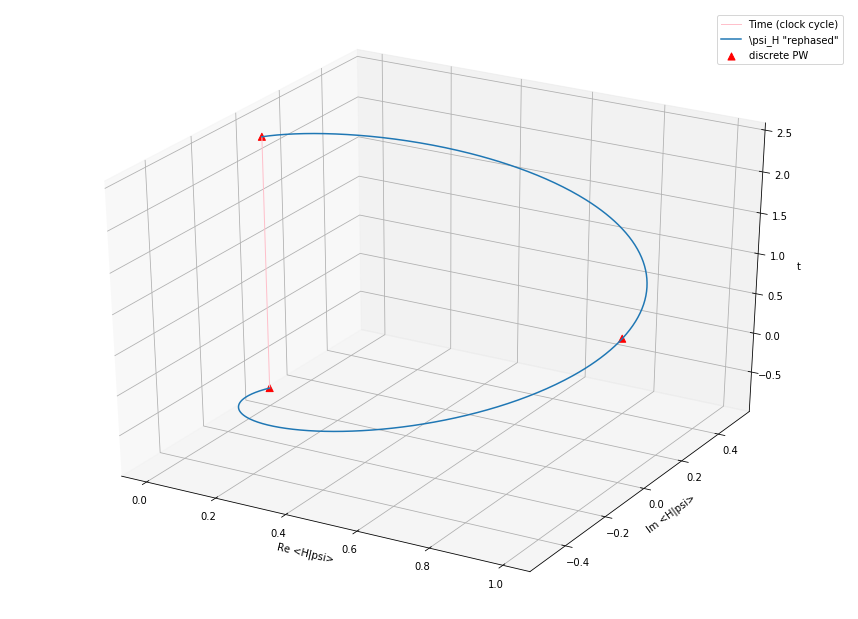
\includegraphics[width=\textwidth/2]{img/psi_H.png}
\caption[(from notebook)]{png}
\end{figure}

\begin{lstlisting}[language=Python]
mpl.rcParams['legend.fontsize'] = 10

fig = plt.figure(figsize=(15, 11))
ax = fig.gca(projection='3d')

# Prepare arrays x, y, z
# z is t
z = np.linspace(-np.pi/4, 3*np.pi/4, 500)

# Auto-broadcasting doesn't work as expected, therefore we explicitly
# map the z vector via `np.vectorize()`

# x is real part of psi[1] or Re(psi_V) as in psi = psi_H|H> + psi_V|V>
x = np.vectorize(lambda t: psi_fixed_1_re(t, -np.pi/4, [0, -1j], 0))(z) 
# y is imag part of psi[0] or Im(psi_H) as in psi = psi_H|H> + ps_V|V>
y = np.vectorize(lambda t: psi_fixed_1_im(t, -np.pi/4, [0, -1j], 0))(z) 

plt.plot([0, 0], [0, 0], [-np.pi/4, 3*np.pi/4], lw=1, c='pink', label='Time (clock cycle)')

ax.plot(x, y, z, label='psi_V "rephased"')

points_x = np.array([     0.0,     0.0,       0.0])
points_y = np.array([    -1.0,     0.0,      -1.0])
points_z = np.array([-np.pi/4, np.pi/4, 3*np.pi/4])
ax.scatter(points_x, points_y, points_z, marker='^', c='red', s=50, alpha=1.0, label='discrete PW')

plt.xlabel(s='Re <V|psi>')
plt.ylabel(s='Im <V|psi>')
ax.set_zlabel('t')

ax.legend()

plt.show()
\end{lstlisting}

\begin{figure}
\centering
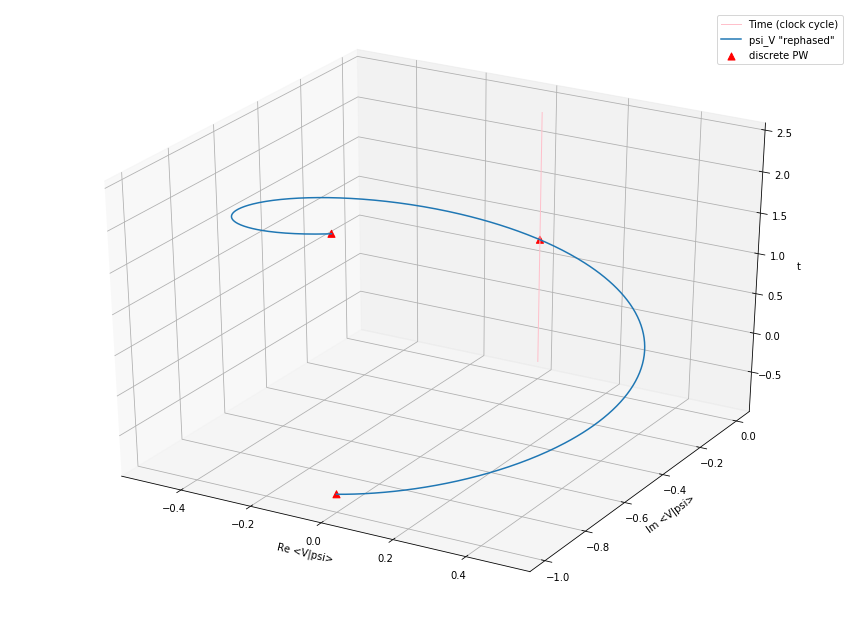
\includegraphics[width=\textwidth/2]{img/psi_V.png}
\caption[(from notebook)]{png}
\end{figure}


\chapter[Mathematica notebooks]{Mathematica notebooks\footnote{
  Ref.: \cite{Wolfram}.
}}
\section*{Preliminary note}

Here we just report the necessary Mathematica commands
and suppress some intermediate outputs,
using \verb#TeXForm[]# otherwise,
in lack of a viable export functionality
available for whole notebooks.

Minimal edit on expressions has been performed for formatting purposes only.
\section[
  \texttt{NN}-level clock $+$ $2$-level system
]{%
  Page--Wootters model: \texttt{NN}-level clock $+$ $2$-level system\footnote{
    Here the symbol \texttt{NN} is used instead of \texttt{N} to avoid confusion with
    Mathematica's \emph{function} \texttt{N[]} which
    is used to convert symbolic expressions to their numerical value.
  }
}
\label{appendix:n-level}

\begin{Verbatim}
NN := 32
\end{Verbatim}

\begin{Verbatim}
T := DiagonalMatrix[Range[0,NN-1]] * \[Pi] / 16
\end{Verbatim}

\begin{Verbatim}
F := FourierMatrix[NN]
\end{Verbatim}

For simplicity, $\hbar = \omega = 1$

\begin{Verbatim}
\[CapitalOmega] := F.T.F\[ConjugateTranspose]  * 16 / \[Pi]
\end{Verbatim}

Hamiltonian in "ordinary" space
\begin{Verbatim}
Hs := \[ImaginaryI]{{0, 1}, {-1, 0}}
\end{Verbatim}
\begin{Verbatim}
MatrixForm[Hs]
\end{Verbatim}
\[
  \left(
    \begin{array}{cc}
     0 & i \\
     -i & 0 \\
    \end{array}
    \right)
\]

Matrix representation of \cite[eq. 1]{Lloyd:Time}.
We turn it into numeric (\verb!N[ ]!) as treating  it symbolically onwards would be unfeasible:
\begin{Verbatim}
J := N[KroneckerProduct[\[CapitalOmega],IdentityMatrix[2]] + KroneckerProduct[IdentityMatrix[NN],Hs]]
\end{Verbatim}
\begin{Verbatim}
Chop[Eigenvalues[J]]

Out[ ] = {32., 31., 30., 30., 29., 29., 28., 28., 27., 27., 26., 26., 25., 25., 24., 24., 23., 23., 22., 22., 21., 21., 20., 20., 19., 19., 18., 18., 17., 17., 16., 16., 15., 15., 14., 14., 13., 13., 12., 12., 11., 11., 10., 10., 9., 9., 8., 8., 7., 7., 6., 6., 5., 5., 4., 4., 3., 3., 2., 2., 1., 1., -1., 0}
\end{Verbatim}
\begin{Verbatim}
Eigenvalues[J][[40]]

Out[ ] = 12.

Eigenvalues[J][[41]]

Out[ ] = 11.

chosenEigenvector := Eigenvectors[J][[ 40]]

chosenEigenvectorB := Eigenvectors[J][[41]]

Normalization := Sqrt[Abs[chosenEigenvector[[1]]^2] + Abs[chosenEigenvector[[2]]^2] ]

NormalizationB := Sqrt[Abs[chosenEigenvectorB[[1]]^2] + Abs[chosenEigenvectorB[[2]]^2] ]

chosenEigenvectorNormalized  := chosenEigenvector / Normalization

chosenEigenvectorNormalizedB := chosenEigenvectorB / NormalizationB  

probability := Abs[chosenEigenvectorNormalized ^2]

probabilityB := Abs[chosenEigenvectorNormalizedB^2]

ListPlot[probability,
  GridLines ->{Range[0,NN*2, 2], Range[0, 1, 0.1]},
  AxesLabel->{n, "P(0), P(1)"},
  LabelStyle->Directive[16],
  PlotMarkers->{Automatic, 16},
  ImageSize->1024
]
\end{Verbatim}
\begin{figure}[!h]
  \centering
  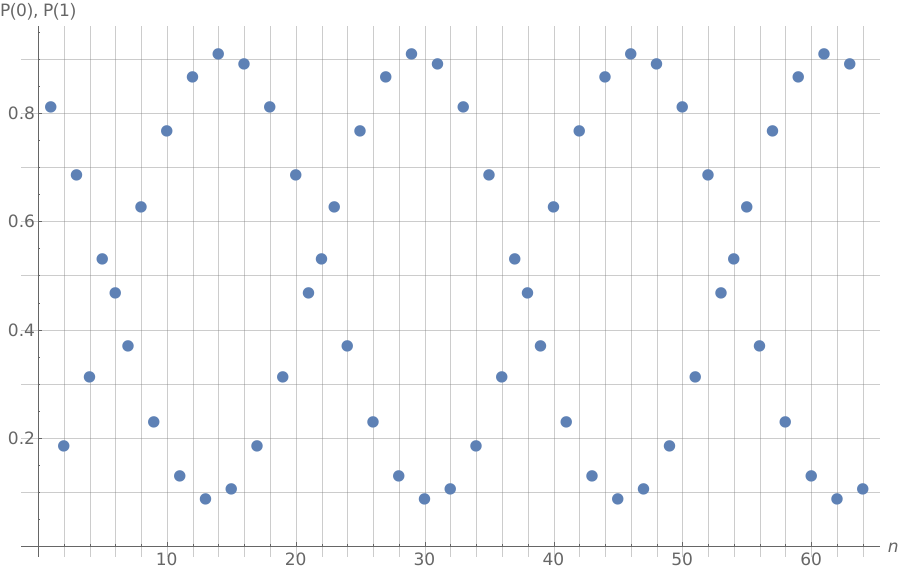
\includegraphics[width=.75\textwidth]{img/N32.png}
  \caption[]{png}{P-W ``evolution'' for $\hat{\mathbb{J}}$ eigenvalue $=12$}
\end{figure}  
\begin{Verbatim}

ListPlot[probabilityB,
  GridLines ->{Range[0,NN*2, 2], Range[0, 1, 0.1]},
  AxesLabel->{n, "P(0), P(1)"},
  LabelStyle->Directive[16],
  PlotMarkers->{Automatic, 16},
  ImageSize->1024
]
\end{Verbatim}
\begin{figure}[!h]
  \centering
  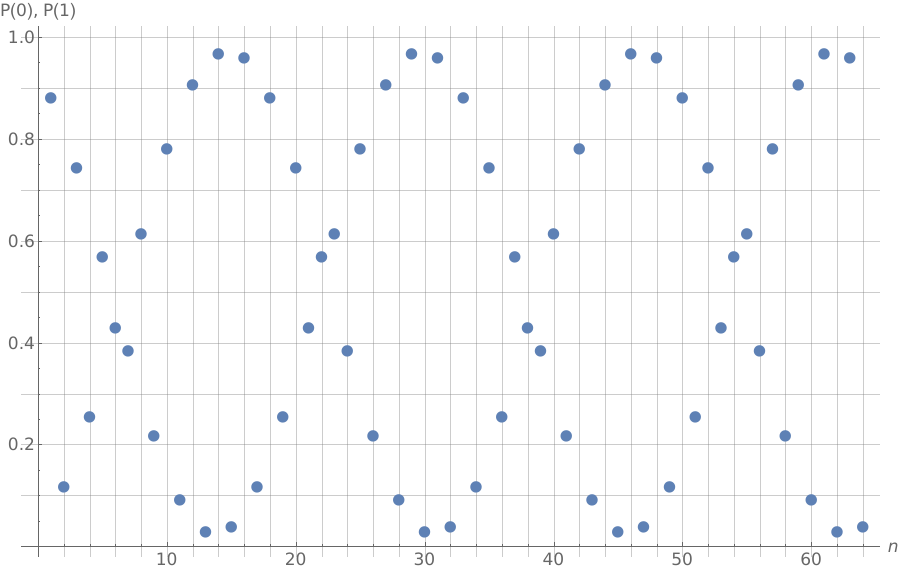
\includegraphics[width=.75\textwidth]{img/N32-B.png}
  \caption[]{png}{P-W ``evolution'' for $\hat{\mathbb{J}}$ eigenvalue $=11$}
\end{figure}

\subsection{Consistency of PW with ordinary QM (discrete approximation)}

\begin{Verbatim}
psi0 :=  chosenEigenvectorNormalizedB[[{1,2}]]
\end{Verbatim}

\begin{Verbatim}
psi[t_] := MatrixExp[-I Hs t, psi0 ]
\end{Verbatim}

\begin{Verbatim}
Plot[(Abs[psi[t]]^2)[[1]],{t,0,2\[Pi]},
  AxesLabel->{t, "P(0)"},
  LabelStyle->Directive[16],
  ImageSize->900
]
\end{Verbatim}
\begin{figure}[!h]
  \centering
  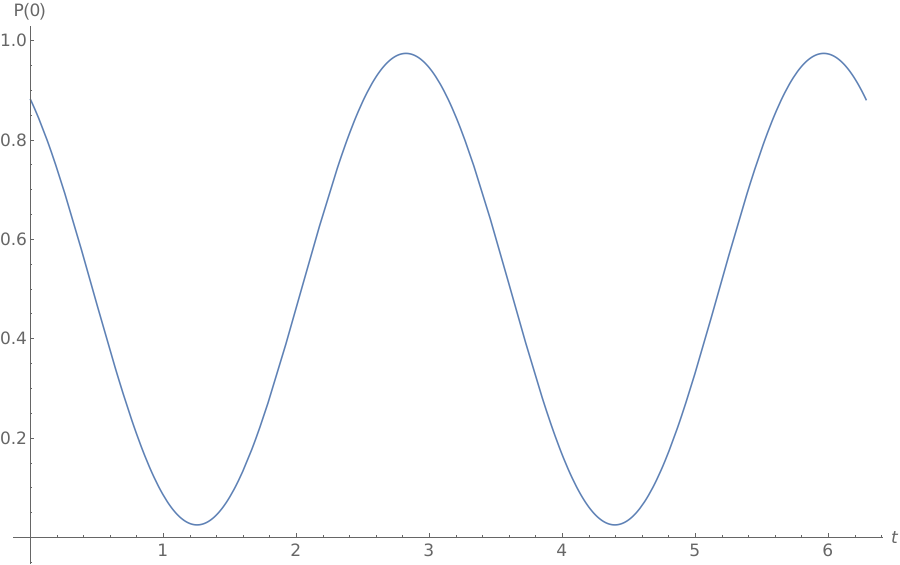
\includegraphics[width=0.75\textwidth]{img/probB_0.png}
  \caption[]{png}{
    Schr{\"o}dinger evolution of
    $\qty|\braket{0}{\psi(t)}|^2$, $t \in (0, 2\pi) $
    picking the first two components of an eigenvector of $\hat{\mathbb{J}}$
    as the two components of $\psi_{t=0}$ in ordinary Hilbert space.
    Related eigenvalue of $\hat{\mathbb{J}}$ is $11$
  }
\end{figure}

\begin{Verbatim}
Plot[(Abs[psi[t]]^2)[[2]],{t,0,2\[Pi]},
  AxesLabel->{t, "P(1)"},
  LabelStyle->Directive[16],
  ImageSize->900
]
\end{Verbatim}
\begin{figure}[!h]
  \centering
  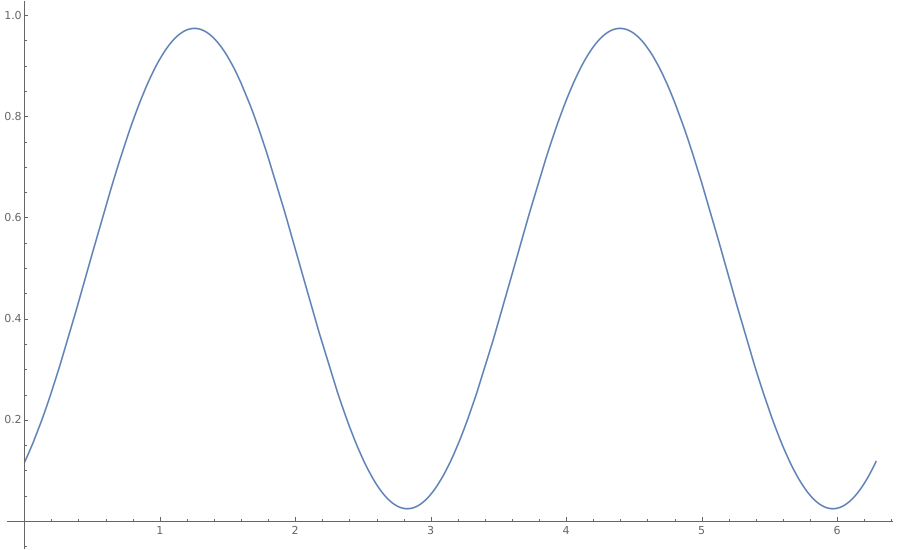
\includegraphics[width=0.75\textwidth]{img/probB_1.png}
  \caption[]{png}{
    Schr{\"o}dinger evolution of
    $\qty|\braket{1}{\psi(t)}|^2$, $t \in (0, 2\pi) $
    picking the first two components of an eigenvector of $\hat{\mathbb{J}}$
    as the two components of $\psi_{t=0}$ in ordinary Hilbert space.
    Related eigenvalue of $\hat{\mathbb{J}}$ is $11$
  }
\end{figure}

\subsubsection{Complex evolution of $\psi$ (not just $\qty|\psi|^2$)}

Please note index count is
$1, 2$ (cells above)
but refers, respectively, to computational base elements
$\ket{0}, \ket{1}$ in ordinary Hilbert space.
\begin{Verbatim}
re0psi[t_] := Simplify[Re[psi[t][[1]]], Assumptions->Element[t, Reals]]
im0psi[t_] := Simplify[Im[psi[t][[1]]], Assumptions->Element[t, Reals]]
re1psi[t_] := Simplify[Re[psi[t][[2]]], Assumptions->Element[t, Reals]]
im1psi[t_] := Simplify[Im[psi[t][[2]]], Assumptions->Element[t, Reals]]
\end{Verbatim}

\begin{Verbatim}
zAxis := ParametricPlot3D[{0,0,t}, {t,0,2\[Pi]}, PlotStyle->{Gray}]
psi0plot := ParametricPlot3D[{re0psi[t], im0psi[t], t}, {t, 0, 2\[Pi]}, PlotStyle->{Red} ]
psi1plot := ParametricPlot3D[{re1psi[t], im1psi[t], t}, {t, 0, 2\[Pi]}, PlotStyle->{Blue} ]
\end{Verbatim}

\begin{Verbatim}
Show[zAxis, psi0plot,psi1plot, ImageSize->Medium,
  AxesLabel -> {
    Style[Re["<0,1|\[Psi]>"], Bold],
    Style[Im["<0,1|\[Psi]>"], Bold],
    Style[t, Bold]
  }
]
\end{Verbatim}
\begin{figure}[!h]
  \centering
  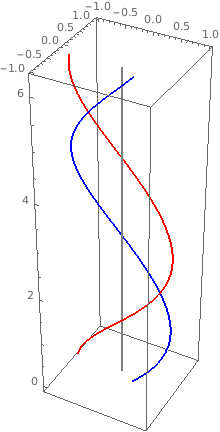
\includegraphics[width=0.25\textwidth]{img/qubit-evo-schrod.png}
  \caption[]{png}{
    Schr{\"o}dinger full complex evolution of components
    $\braket{0}{\psi(t)}$ (red) and 
    $\braket{1}{\psi(t)}$ (blue) for
    $t \in (0, 2\pi) $. The initial state
    has been chosen as the first two components of an eigenstate of
    $\hat{\mathbb{J}}$, related to eigenvalue $= 11$.
  }
\end{figure}

\begin{Verbatim}
pi = N[\[Pi]]

3.14159
\end{Verbatim}

\begin{Verbatim}
rephased[k_] := chosenEigenvectorNormalizedB [[k]] * Exp[-\[ImaginaryI]*pi*11*(k-1)/NN]

rephased1[k_] := chosenEigenvectorNormalizedB [[k]] * Exp[-\[ImaginaryI]*pi*11*(k-2)/NN]

scatter[k_] := {Re[ rephased[k]], Im[ rephased[k]], pi*(k-1)/NN}

scatter1[k_] := {Re[ rephased1[k]], Im[ rephased1[k]], pi*(k-2)/NN}

scatterPoints = Map[scatter, Range[1,2*NN, 2]]

Out[ ] = {{0.891003,-0.00706481,0.}, {0.896671,-0.0925068,0.19635}, {0.86788,-0.174394,0.392699}, {0.805737,-0.249579,0.589049}, {0.71263,-0.315173,0.785398}, {0.592137,-0.368655,0.981748}, {0.448889,-0.40797,1.1781}, {0.28839,-0.431607,1.37445}, {0.116809,-0.438657,1.5708}, {-0.0592618,-0.42885,1.76715}, {-0.233055,-0.402563,1.9635}, {-0.397892,-0.360805,2.15984}, {-0.547438,-0.305182,2.35619}, {-0.675946,-0.237831,2.55254}, {-0.778478,-0.16134,2.74889}, {-0.851094,-0.0786487,2.94524}, {-0.891003,0.00706481,3.14159}, {-0.896671,0.0925068,3.33794}, {-0.86788,0.174394,3.53429}, {-0.805737,0.249579,3.73064}, {-0.71263,0.315173,3.92699}, {-0.592137,0.368655,4.12334}, {-0.448889,0.40797,4.31969}, {-0.28839,0.431607,4.51604}, {-0.116809,0.438657,4.71239}, {0.0592618,0.42885,4.90874}, {0.233055,0.402563,5.10509}, {0.397892,0.360805,5.30144}, {0.547438,0.305182,5.49779}, {0.675946,0.237831,5.69414}, {0.778478,0.16134,5.89049}, {0.851094,0.0786487,6.08684}}

scatterPoints1 = Map[scatter1, Range[2,2*NN, 2]]

Out[ ] = {{0.116809,-0.438657,0.}, {-0.0592618,-0.42885,0.19635}, {-0.233055,-0.402563,0.392699}, {-0.397892,-0.360805,0.589049}, {-0.547438,-0.305182,0.785398}, {-0.675946,-0.237831,0.981748}, {-0.778478,-0.16134,1.1781}, {-0.851094,-0.0786487,1.37445}, {-0.891003,0.00706481,1.5708}, {-0.896671,0.0925068,1.76715}, {-0.86788,0.174394,1.9635}, {-0.805737,0.249579,2.15984}, {-0.71263,0.315173,2.35619}, {-0.592137,0.368655,2.55254}, {-0.448889,0.40797,2.74889}, {-0.28839,0.431607,2.94524}, {-0.116809,0.438657,3.14159}, {0.0592618,0.42885,3.33794}, {0.233055,0.402563,3.53429}, {0.397892,0.360805,3.73064}, {0.547438,0.305182,3.92699}, {0.675946,0.237831,4.12334}, {0.778478,0.16134,4.31969}, {0.851094,0.0786487,4.51604}, {0.891003,-0.00706481,4.71239}, {0.896671,-0.0925068,4.90874}, {0.86788,-0.174394,5.10509}, {0.805737,-0.249579,5.30144}, {0.71263,-0.315173,5.49779}, {0.592137,-0.368655,5.69414}, {0.448889,-0.40797,5.89049}, {0.28839,-0.431607,6.08684}}
\end{Verbatim}

\begin{Verbatim}
scatterPlot = ListPointPlot3D[scatterPoints, PlotStyle->{Red, PointSize[Large]}]
\end{Verbatim}
\begin{figure}[!h]
  \centering
  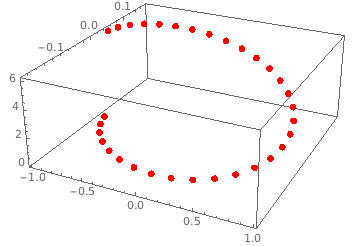
\includegraphics[width=0.4\textwidth]{img/scatterplot0.png}
  \caption[]{png}{
    Page--Wootters discrete-time evolution of
    $\braket{0}{\psi(t)}$ in 32 points between
    $t \in (0, 2\pi) $. From an eigenstate of
    $\hat{\mathbb{J}}$ related to eigenvalue $\epsilon = 11$.
    The evolution has been ``corrected'' via a phase oscillation
    factor $e^{-i \epsilon t}$
    as explained in \cite[\it ``The Zero-eigenvalue'']{Lloyd:Time}.
  }
\end{figure}

\begin{Verbatim}
scatterPlot1 = ListPointPlot3D[scatterPoints1, PlotStyle->{Blue, PointSize[Large]}]
\end{Verbatim}
\begin{figure}[!h]
  \centering
  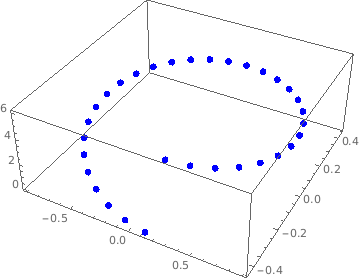
\includegraphics[width=0.4\textwidth]{img/scatterplot1.png}
  \caption[]{png}{
    Page--Wootters discrete-time evolution of
    $\braket{1}{\psi(t)}$ in 32 points between
    $t \in (0, 2\pi) $. From an eigenstate of
    $\hat{\mathbb{J}}$ related to eigenvalue $\epsilon = 11$.
    The evolution has been ``corrected'' via a phase oscillation
    factor $e^{-i \epsilon t}$
    as explained in \cite[\it ``The Zero-eigenvalue'']{Lloyd:Time}.
  }
\end{figure}

\begin{Verbatim}
Show[zAxis, psi0plot,psi1plot,scatterPlot, scatterPlot1, ImageSize->Large,
  AxesLabel->{
    Style[Re["<0,1|\[Psi]>"], Bold],
    Style[Im["<0,1|\[Psi]>"], Bold],
    Style[t, Bold]
  }
]
\end{Verbatim}
See Figure \ref{fig:complex-comparison}.

% references
\printbibliography[heading=bibintoc]

\end{document}
